\chapter[Learning and War]{Learning and War: Applying Learning Models to the International Interaction Game}

\section{Background}\label{background}

An important topic in the study of international relations is how the actors in the international system (primarily countries) make decisions when interacting with one another. One common view, most often associated with the Realist schools of thought \citep{sep_2013} is that states\footnote{I will use states and countries interchangeably to refer to sovereign, territorial political entities.} are rational: they act in a way that attempts to maximize their utility, often defined as security from the threat of attack by other states \citep{keohane_1986}. Many critiques of Realist theories, particularly from the Liberal perspective \citep[e.g.][]{keohane_1987}, focus on disputing the constraints and goals faced by states and on whether states are even the correct actors to concentrate on, but not that the relevant actors themselves are rational. Nevertheless, there has also been substantial scholarship arguing against the idea of states as rational, goal-directed actors, focusing both on the differing objectives and relationships of the internal actors involved in the decisionmaking process \citep{singer_1961,wendt_1987,allison_1999}, and on the psychological biases of the individuals who are, ultimately, the ones making the decisions \citep{north_1967,jervis_1976,khong_1992,kaufmann_1994}.

Crises, and the precipes of conflict between countries, are particularly important phenomena. The decision to threaten or use force is one of the most consequential external decisions a state may make, and the substantial costs and consequences of wars at the national and human levels make them compellingly important to study, explain, and possibly even predict or avert. In ``The Essence of Decision,'' \citet{allison_1999} closely examined one particularly important example: the 1962 Cuban Missile Crisis, in which the world's two superpowers, the United States and the Soviet Union, faced a series of decisions to initiate or escalate a military confrontation with one another that had a real possibility of leading to a nuclear exchange. The book reviews three models of state decisionmaking: rational choice, where the decisionmakers attempt to evaluate various possible courses of action and choose those which have the highest expected utility, while taking the adversary's responses into account; organizational behavior, wherein the states' decisions are driven by standing institutional procedures; and governmental politics, in which decisions are driven by competition between internal factions and actors with different interests and degrees of influence. The book demonstrates that all three models can provide convincing explanations of the behavior of the United States and Soviet Union over the course of the crisis, and in particular that the latter two models can explain actions that do not make sense as strategic, security-maximizing decisions. Similarly, \citet{kaufmann_1994} conducted a detailed case study of another international crisis, the 1905-06 Moroccan Crisis (wherein Germany attempted to undermine French influence in Morocco and brought Europe to the brink of war), and used archival sources to argue that the key German decisionmakers updated their views and positions during the crisis in response to events and new information in a way that is inconsistent with pure rationality, but consistent with the psychological biases expected to affect them.
% WGK: Consider breaking up EoD models into bullet points or something?

Both of these examples demonstrate the power of comparative analysis of different decisionmaking models, and especially the application of multiple models to the same case. However, both share a reliance on qualitative analysis of detailed primary sources detailing not only the ultimate behavior of the state-level actors but the internal deliberations of their decisionmaking individuals and organizations. This makes it difficult to test these models across different cases, or to use them to make broad hypotheses as to the conditions under which we can expect conflicts or predict how they will be resolved. In this, they are nearly the complete opposite of game theory, perhaps the other methodological pole in the study of international relations. 

Game theory is the mathematical study of models of interactions (games) between multiple actors (players), where the payoff each player receives depends on the combination of their own actions and those of the other players. Game theory generally takes utility-maximizing rationality as axiomatic; this allows games to be analyzed in order to identify and characterize their equilibrium -- the outcome of a game when all players are perfectly rational, know that the other players are perfectly rational as well, and figure out the best possible course of action given that the other players are doing the same thing. Recently, however, behavioral game theory \citep{camerer_2003} has sought to use experiments and psychological insights to study how humans actually approach such games, and how their behavior differs from theoretical, rational expectations.

%Much of modern game theory was developed in order to study international conflict \citep{gates_1997}.  Game theory takes utility-maximizing rationality as axiomatic, and much of the work of game theory involves studying games (formal models of interaction) in order to identify and characterize their equilibrium -- the outcome of a game when all players are perfectly rational, know that the other players are perfectly rational as well, and figure out the best possible course of action given that the other players are doing the same thing. Game-theoretic models tend to be highly abstract, and may provide useful analogies and theory-generating insights rather than specific explanations or predictions applicable to a particular case \citep{snidal_1985}.

% RAX: Slightly awkward introduction to game theory -- rewrite to explicitly emphasize game theory as the font of rational modeling; maybe note behavioral game theory?
% RAX: Cite Gintis on game theory as a general social science?

Game-theoretic models tend to be highly abstract, and may provide useful analogies and theory-generating insights rather than specific explanations or predictions applicable to a particular case \citep{snidal_1985}. An important exception is included in ``War and Reason'' by \citet{bdm_1992}, which presents the International Interaction Game: a game-theoretic, extensive-form model of inter-state crises. The game consists of two agents sequentially choosing whether to escalate confrontation or attempt to deescalate, with outcomes ranging from the maintenance of the status quo (when neither actor escalates at all) to war (when both actors escalate as far as possible). While much of the book is devoted to conventional formal analysis of the model and its equilibria under different parameters, the authors also test the theory empirically. They propose a methodology to estimate the game's payoffs for any given pair of states, using data on the states' alliances to measure the conflict stakes,  and states' material capabilities to measure the strength each side and its allies can bring to bear. Using this methodology with historic data from the Correlates of War project, they estimate the game payoffs for 707 historic European dyads (pairs of countries in a particular year) from the 1816-1970 time period. They find the equilibrium outcome for each, and show that these outcomes are useful predictors of the corresponding event observed between those countries for that year. \citet{bennett_2000b} developed a software tool expanding the estimation to all historic dyads across the entire international system between 1816 and 1992, largely confirming that the estimated equilibria can be used to predict the observed event for the corresponding dyad -- though the strongest predictions required controlling for distance, great power status, and other relevant factors.

Agent-based models have seen relatively limited use in the study of international relations, and have generally been applied similarly to game-theoretic models. Many \citep[e.g.][]{cederman_1997,axelrod_1997,min_2002} involve simulations of notional, simplified international systems, with agents acting in accordance with some particular theories. These models provide stylized insights into what patterns emerge (or do not) from these theories, but are not meant to directly describe specific real-world countries or conflicts. One important example is the \citet{axelrod_1980} Prisoners' Dilemma Tournament, which explicitly sought to compare the performance of different behavior rules playing an iterated game. While this research utilized a simple theoretical model, it was done with an eye towards the study of, among other issues, international conflict and cooperation. Similarly, though less robustly, \citet{cederman_1997} involves competition between agents with two sets of behavioral rules, those content with the status quo and those seeking to expand at the expense of their neighbors. These experiments demonstrate a powerful feature of agent-based models, which has heretofore been underutilized in political models: the ability to have agents using different behavior models interact and compete with one another within a common context.

While it is not presented as such, the \citet{bdm_1992} empirical application of the International Interaction Game bears some similarity to an ABM. Indeed, the empirical application of the model is only feasible computationally. It consists of distinct, unitary actors with well-specified decision rules, carrying out discrete interactions with one another. These interactions, in turn, generate a series of cooperative and conflictual behaviors, which can be compared to empirical data. Nevertheless, as previously implemented by \citet{bdm_1992} and \citet{bennett_2000,bennett_2000b}, the agents (such as they are) only feature a single decisionmaking model, rationally playing the equilibrium moves. The way I will extend the International Interaction Game (IIG) should now be clear: I propose to reimplement the model explicitly as an agent-based model, and to do so in a way that allows me to endow agents with  different decisionmaking models and rules, drawn from different theories of state behavior. Utilizing the IIG game tree and payoff estimates keeps the model anchored to a well studied, empirically validated foundation. I then use this framework to simulate the same set of interactions using different decisionmaking models, obtaining sets of outcomes for each variant. These outcomes can be compared to one another to see where and how they differ, and to empirical data, to see which provides the best fit.

% RAX: Cite Green & Shapiro (green_1994, pathologies... rat. choice) here?

In this framework, formal rationality will be the initial decisionmaking model I will implement. As discussed above, this is the default model of decisionmaking used in game-theoretic models. It serves as an operationalization of the qualitative rational choice model as described by \citet{allison_1999} and many others. The analysis in \citet{bennett_2000} compares the explanatory power of the overall IIG to dyad-level variables (e.g. geographic distance, government types) but not to other models of decisionmaking. Here, in contrast, using rationality as a baseline will allow us to directly test whether the additional decisionmaking models provide stronger explanatory power than the rational decisionmaking model itself. Furthermore, reimplementing the rational choice model will serve as a form of verification, ensuring that my model framework is producing the same results as the \citet{bennett_2000,bennett_2000b} implementation.

I implement two alternative models of decisionmaking within this framework. The first variant is a stylized representation of the organizational procedure model described by \citet{allison_1999} and \citet{levy_1986}: agents develop standard operating procedures, which they apply regardless of the specifics of each interaction they find themselves in. These procedures are updated based on the outcome of the new interaction, such that successful courses of action will be more likely to be executed in the future, and unsuccessful ones less likely.

The second variant implements a stylized version of the theory described by \citet{march_1993} and \citet{khong_1992} by which organizations, and states in particular, make decisions by comparing their present circumstances to previous similar cases they encountered. In this variant, the agents maintain a library of past interactions, which they draw on to make decisions about each new interaction. If a course of action was successful in a similar previous interaction, the agent will be more likely to use it again; otherwise, they will be more likely to attempt an alternative.

These decisionmaking models are both implemented using reinforcement learning. This methodology has several advantages: it originates from psychology, but has had success as a machine learning technique \citep{sutton_1998}. Reinforcement learning agents have been shown to be capable of learning to play extensive-form games \citep{laslier_2005,akramizadeh_2009}, as well as to learn to cooperate and compete in multi-agent environments \citep{littman_1994,claus_1998}. They have been used to model the learning of individuals and groups of decisionmakers \citep{kocher_2005}; however, they are not always successful at learning to play the equilibrium of abstract, normal-form games, and in fact can yield unexpected and even chaotic behavior \citep{galla_2013}. Furthermore, \citet{khong_1992}, \citet{allison_1999}, and \citet{cederman_2001} have observed that states as a whole (rather than just individual decisionmakers) exhibit a degree of learning from past experiences. In short, reinforcement learning provides a plausible, general model of decisionmaking which is not procedurally rational \citep{simon_1976}, but introduces minimal additional assumptions as to the form the behavior takes. Additionally, reinforcement learning makes minimal assumptions as to the structure of the game the agents are playing, meaning that a single behavior model may be implemented once and used to drive agents across different games and other interaction models. %% Add citation for temporality in IR?

The question I set out to explore here is whether reinforcement learning agents interacting with one another over a series of simulated international crises can converge to behavior resembling the equilibria for those interactions. If this is the case, it will suggest a degree of convergence between the rational choice, psychological, and organizational models of decisionmaking. If it is not, however, it will diverge, generating different results which may then be tested against empirical data. In the course of addressing these questions, I will also lay out a more general architecture and methodology for extending game-theoretic models of international crises into agent-based models, which can be used to implement and test additional models of decisionmaking. As \citet{allison_1999} write, ``because  simplifications are necessary, competing simplifications are essential.'' In this chapter, I will present a methodology for extending the competing simplifications from the realm of case studies to computational modeling.

This chapter is organized as follows. In Section \ref{description}, I present the general architecture for an agent-based model of dyadic, extensive-form interactions with variable agent decisionmaking. I describe two simulated worlds: a simplified, notional international system (Section \ref{small_crisis}), and a more complicated data-grounded historic simulation based on \citet{bdm_1992} and \citet{bennett_2000} (Section \ref{sec:iig_description}). I then present several behavior variants, grounding them both in political and multi-agent theory (Section \ref{decisionmaking_models}). In Section \ref{small_crisis_results}, I apply these behavior variants to the notional model and verify their behavior, and then apply them to the full historic data in Section \ref{iig_results}. I compare their behavior to the purely rational decisionmaking, and to the observed historic outcomes of each simulated interaction.

\section{Model Description} \label{description}

The overall model I present here consists of three sub-models intended to capture distinct levels of phenomena: the `World' consisting of a set of agents with certain properties, which may be fixed or change over time; the Interaction sub-model, consisting of an extensive-form game tree for pairs of agents to play against each other; and the Agents themselves. The Agent class, in turn, is composed of two parent classes: the World Agent, which defines the properties and methods specific to the World, and a Decisionmaking Model, which the agents utilize to play the extensive-form game at each interaction. All these sub-models are implemented initially as abstract classes, which include the methods common across all model variants; these abstract classes are then sub-classed and implemented for each model variant. Figure \ref{fig:model_architecture} shows a UML class diagram tying together these different classes.

\begin{figure}[h!]
    \centering
	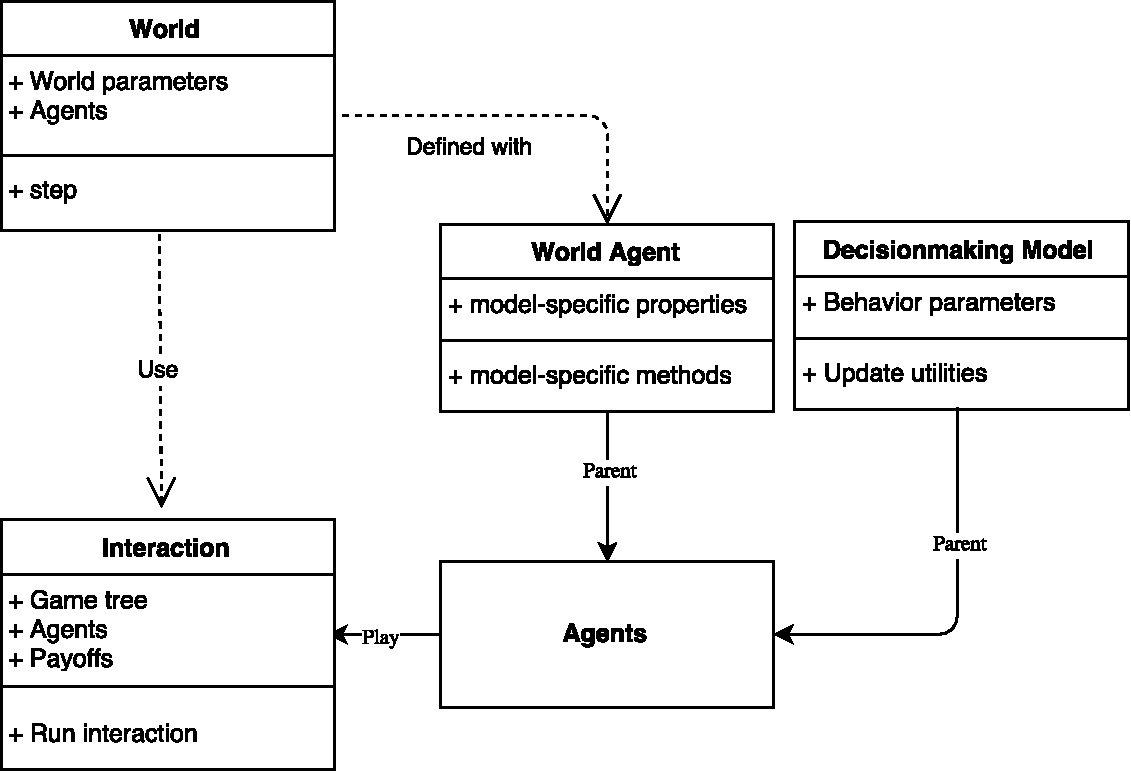
\includegraphics[width=0.75\textwidth]{WarReason/Figures/ModelArchitecture}
    \caption{Model Architecture}
    \label{fig:model_architecture}
    \figSpace
\end{figure}

\subsection{World Sub-Model}

The World sub-model acts as the overall controller for the entire model. It stores and manages the agents who will interact with each other over the course of each instantiation, generating a particular notional history. A World is instantiated with a set of agents, as well as a subclass of the generic Interaction sub-model class, described below. The World implementation can also accept additional data used to generate agents, schedule their interactions, and store and export the outcomes of those interactions.

The World's key method is the `step', which advances the model by one simulated year, chosen since that is the level at which the IIG data is available. Each year consists of some set of interactions, depending on the model variant. For example, these may be some number of random pairings of agents, all possible agent dyads, or pairings based on crises occurring in the given year as recorded in the input data. The agents do not directly choose with whom or when to interact; the interaction scheduling is exogenous to the agents themselves. Since the player order matters in extensive-form games, the interaction dyads are directed -- that is, an interaction between A and B is not the same as one between B and A.

Finally, the World also collects and stores data on each agent, and on the result of each interaction -- that is, which terminal node the interaction ended up on, as explained below. A World implementation may also perform some evaluation on this interaction outcome. In particular, the World sub-models I develop compare the outcome of each interaction to that interaction's equilibrium outcome.

\subsection{Interaction Sub-Model}

This is the core of the overall model: a single interaction between agents playing through a standard, two-player, extensive-form game \citep{shoham_2009}. An interaction model is implemented with a game tree, and methods for computing the payoff to each agent at each terminal node. The game tree here is assumed to be a direct, acyclic graph with perfect information (that is, there are no information sets of more than one node, and agents know exactly the node where the game is currently). The player agents take turns in fixed order, and there are also no moves by nature.

Each agent has a step method, which takes the interaction state as an input and emits a move. The sub-model makes sure that the move is valid for the current node, and advances the game's current node to the appropriate result of the given move. If this is a terminal node, the interaction is over, and payoffs are distributed to all the agents. Otherwise, the next player agent is called.

I use two game trees here, which are shown in Figures \ref{fig:small_crisis_tree} and \ref{fig:iig_tree}. The simpler one is drawn from \citet{signorino_1999}, and will be used for the notional model; the more complicated one is from \citet{bdm_1992} and will be applied to the historic data. The utility calculations associated with both will be provided in more detail in the appropriate sections below.

\subsection{Agent Sub-Model}

Finally, there are the agents themselves. Each agent is meant to represent one actor in the international system, as they interact with one another as described above. Each agent class has two parent classes, as shown in Figure \ref{fig:model_architecture}: one is the World Agent, for the particular model variant which provides its properties; the second is the Decisionmaking Model, which contains the methods and properties the agent uses to make decisions at each step of the game. All agents in a given World must have the same World Agent parent, which is compatible with the Interaction sub-class. However, different agents within a world may have different decisionmaking parents.

In general, the agent properties deriving from the model variant parent class are used to compute the utilities the agent expects from each terminal node in the game tree. The decisionmaking parent, in turn, provides the `step' method, with which the agent chooses its next move through the game tree during an interaction. This structure allows decisionmaking rules to be modeled once, verified, and applied across different specific interaction and world models with minimal additional development. 

\section{Model Variants}

I present two model variants below. Each one consists of an implementation of the three sub-models described above: a World, Interaction model, and agent properties. The first variant, the Small Crisis Game, is a simple notional model used for testing the agent behaviors under controlled conditions. The second, the International Interaction Game, is a full model of the international system extending \citet{bdm_1992} and \citet{bennett_2000b}, at a level of one agent per state, attempting to capture historic interaction dyads.

\subsection{Small Crisis Game} \label{small_crisis}

This model variant is a purposeful simplification: in the number of agents, their properties, and the game tree of their interactions. It is adapted from \citet{signorino_1999}, which in turn adapts the game tree shown in Figure \ref{fig:small_crisis_tree} from the game trees in \citet{bdm_1992}, as well as \citet{kim_1995} and \citet{fearon_1995}. At every node of this game tree, agents (Players 1 and 2, or P1 and P2) may escalate the conflict (fight, $F$) or refrain from escalating (not fight, $!F$). If neither agent chooses to escalate, the result is the Status Quo; if one agent escalates, the other agent faces a choice between not escalating and yielding to the escalator's demand (Capitulating), or fighting, leading to War. These outcomes are the tree's terminal nodes.

The payoffs associated with these terminal nodes are dependent on agent properties. Each agent $i$ in this model is defined by its Assets ($a_i$), indicating what they have that other agents might want (whether territory, material, or more abstract positions or concessions); their Capability ($c_i$), indicating the strength they have to coerce other agents and defend themselves from coercion by others; and a Bloc ($b_i$), where two agents are geopolitically aligned (and have more incentive to cooperate) if their Bloc properties match. These properties are used to compute the utilities associated with each terminal node, as shown in Table \ref{table:smallcrisis_utils}. These utilities are also adapted from \citet{signorino_1999}: when agents capitulate, they yield the assets being contested, with the other agent gaining them. If the agents enter into conflict, they will win with probability based on the ratio of their capability to the other agent's; if they win, they secure the other agent's assets -- and if they lose, they lose not only the value of their own assets, but of their expended capability as well. The Status Quo leads to no change in utility if the agents belong to different blocs; however, if the agents belong to the same bloc, cooperation (i.e. not entering into conflict) has a positive payoff\footnote{In \cite{signorino_1999}, there is a Democracy property instead of a Bloc property, with only dyads of democracies receiving the cooperation payoff; the form I present here is more general, and does not introduce the assumption of democratic peace. However, initial experiments using the original specifications produced substantively similar results to the ones I present here.}.

\begin{figure}[h!]
    \centering
	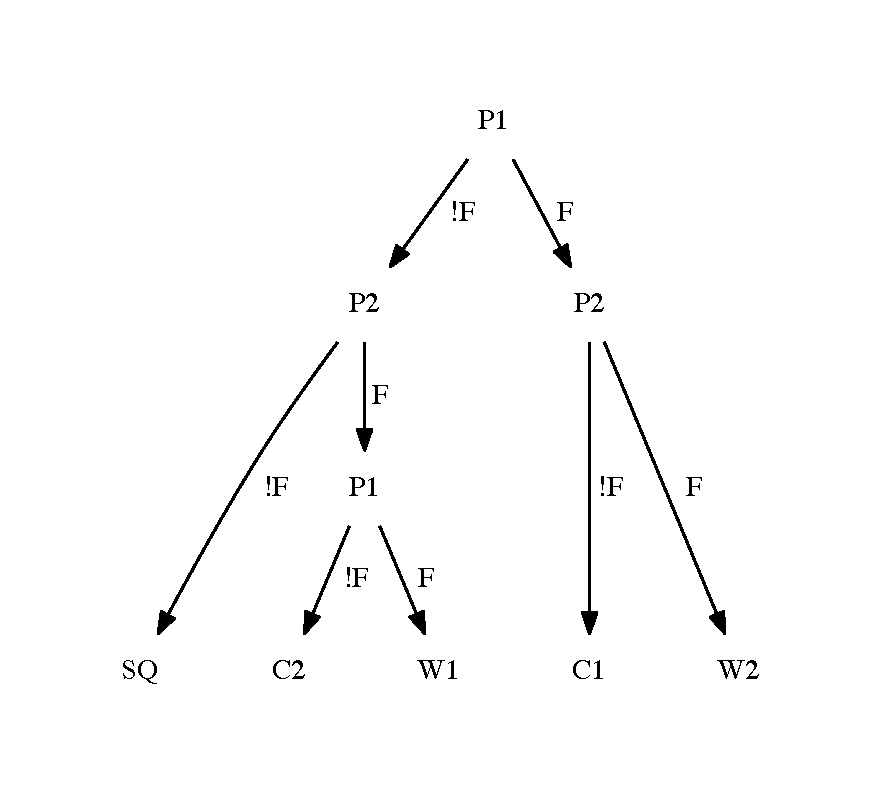
\includegraphics[scale=0.75]{WarReason/Figures/SmallCrisisTree}

    \caption[Small Crisis Game Tree]{Small Crisis Game Tree \citep[adapted from][]{signorino_1999}}
    \label{fig:small_crisis_tree}
    \figSpace
\end{figure}


\begin{table}[h!]
\centering
  \caption{Small Crisis Model Utilities}
  \label{table:smallcrisis_utils}
\begin{tabular}{lll}
	\hline
	Node 			& $U_1$ 		& $U_2$ \\
	\hline
	Status Quo (SQ)  	& $20\delta(b_1,b_2)$			&	$20\delta(b_1,b_2)$			\\
	Capitulate 1 (C1)	& $-a_1$						& $a_1$							\\
	Capitulate 2 (C2) 	& $a_2$							& $-a_2$						\\
	War 		 (W1, W2)	& $p_1a_2 + (1-p_1)(-a_1-m_1)$  & $p_2a_1 + (1-p_2)(-a_2-m_2)$	\\
	\hline
	$p=$Prob(win)	& $\frac{c_1}{c_1+c_2}$ 	   	& $\frac{c_2}{c_1+c_2}$			\\
	\hline
\end{tabular}
\tableSpace
\end{table}

For every instantiation of the CrisisWorld, $N$ agents are generated at random, with random properties drawn uniformly as shown in Table \ref{table:agent_properties}. These agents will persist across the entire run; that is, agents are not added to or removed from the model instance. In each instantiation, all agents will share the same decisionmaking model, as specified below.

Each year of the model (that is, a step of the world), all the agents will be paired up, in random order. Since the number of agents being simulated is substantially smaller than the total number of agents in the international system, this can be thought of as representing a particular region (analogous to the focus on European dyads in \citet{bdm_1992}), or a subset of politically-relevant actors within a larger system.

\begin{table}[]
\centering
	\caption{Small Crisis Agent Properties}
  	\label{table:agent_properties}
\begin{tabular}{lll}
	\hline
	Property & Distribution 	 & Change  	 \\
	\hline
	$a_i$	 &	$Unif\{1, 100\}$ & $\mathcal{N}(0, 5)$   \\
	$c_i$	 &	$Unif\{1, 100\}$ & $\mathcal{N}(0, 5)$	 \\
	$b_i$	 &	$Bernoulli(0.5)$ & $1 - Bernoulli(0.05)$ \\
	\hline
\end{tabular}
\tableSpace
\end{table}

I create two variants of the Small Crisis model. In the first, the Static variant, the agent properties are fixed across each run. In the second, the Dynamic variant, the properties of each agent change stochastically at the beginning of every simulated year, with the changes distributed as shown in Table \ref{table:agent_properties}. This means that under the first variant, the utilities (and hence the equilibrium) of an interaction between each dyad of agents are constant, whereas in the second variant they may drift from step to step.

Note that the agent attribute values do not change due to the results of their interactions. While this is a simplifying assumption, it also corresponds to the dynamics observed in the National Material Capabilities dataset \citep{singer_1988,grieg_2010}, wherein the majority of conflicts do not substantially impact states' estimated material capabilities or alliance relationships -- which are used in the empirical International Interaction Game to operationalize the capabilities of states and the stakes of conflict, respectively, as described below.

\subsection{International Interaction Game} \label{sec:iig_description}

The International Interaction Game, as described in \citet{bdm_1992} is as follows. It involves two actors, one who initiates the interaction and one who responds. The game proceeds following a tree, as shown in Figure \ref{fig:iig_tree}. As in the simplified model, at each node the actors (Players 1 and 2, P1 and P2) have a choice between two moves: escalating the confrontation (fight, $F$) or not escalating ($!F$). There are more nodes in this tree, leading to a wider range of outcomes. If neither actor escalates, the result is still the Status Quo, while if both consistently escalate the result is War. If one agent yields to the other's escalation early on, the outcome is Acquiescence, while if they yield after a greater degree of escalation, the outcome is Capitulation, with some additional cost incurred. If both actors initially escalate and then deescalate, the result is a negotiated compromise. 

\begin{figure}[h!]
    \centering
	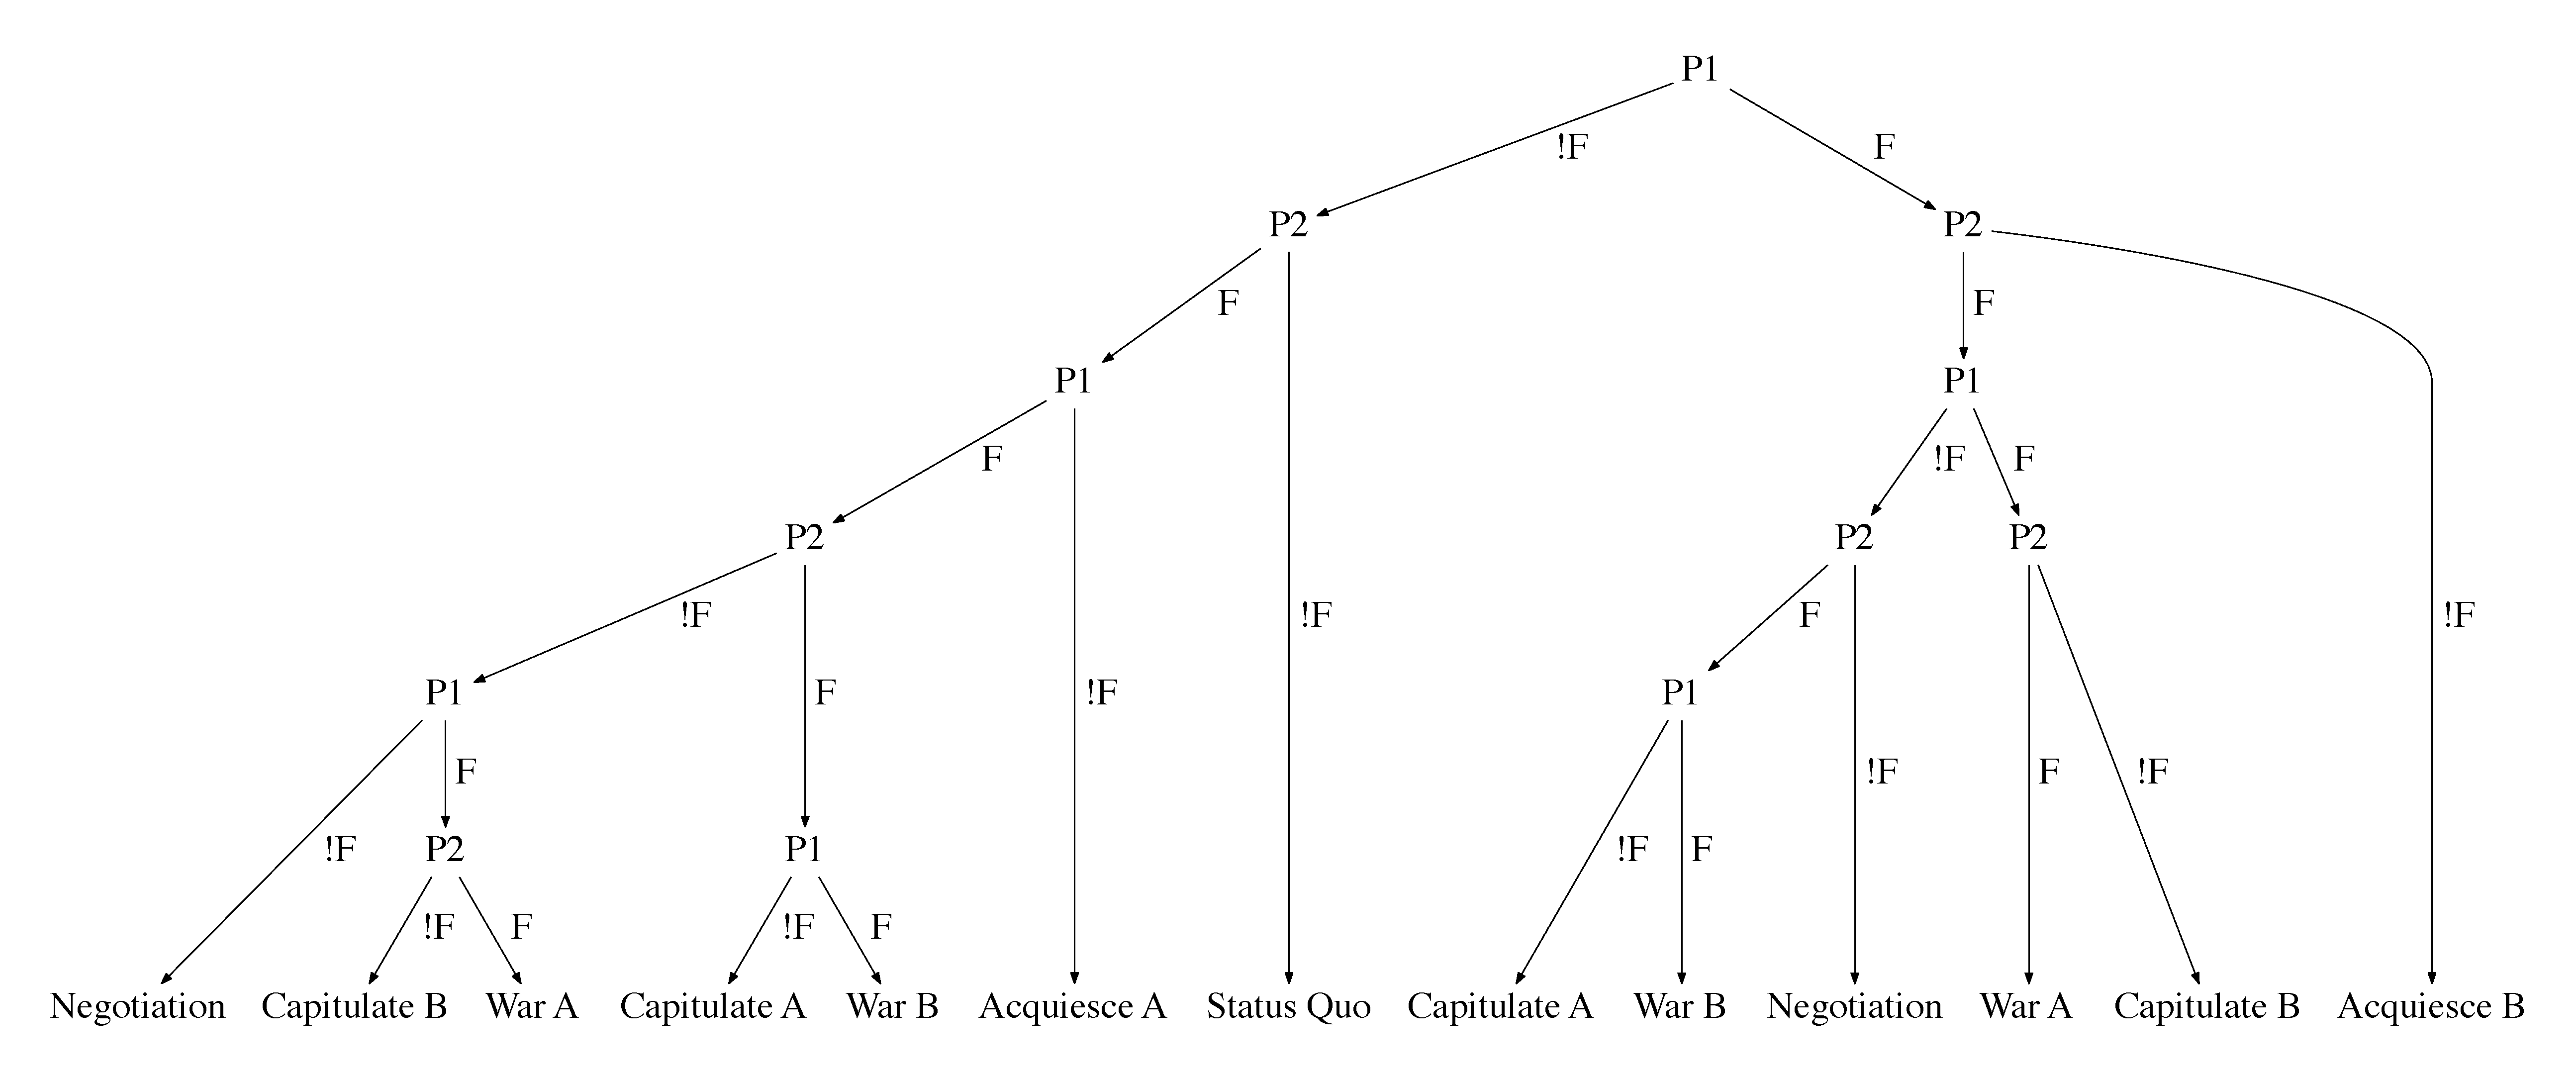
\includegraphics[width=\textwidth]{WarReason/Figures/IIGTree}

    \caption[International Interaction Game Tree]{International Interaction Game Tree \citep[from][]{bdm_1992}}
    \label{fig:iig_tree}
    \figSpace
\end{figure}

While each interaction is dyadic, the utilities of each outcome for both actors are determined by the overall international system the interaction occurs within, and specifically the network of alliances. Alliances are used as a proxy for states' interests. The COW alliance data \citep{singer_1969} records the type of each formal alliance each state has with any other state in a given year; this is that state's alliance portfolio. As \citet{bdm_1975} argues, two states with similar interests can be expected to have similar alliance portfolios -- that is, many of the same types of alliances with the same other states. \citet{bdm_1992} uses a standard statistical similarity measure known as Kendall's tau-b to compute this similarity, though \citet{signorino_1999b} argues that this measure is inadequate, and proposes an alternative. To maintain consistency with \citet{bdm_1992} and \citet{bennett_2000}, I will use Kendall's tau-b, denoted below as $K_{i,j}$ -- the similarity between actors $i$ and $j$'s alliance portfolios. However, other similarity measures, such as those proposed by \citet{signorino_1999b} may be substituted as well.

The estimated similarity between the two states is used to determine the two base utility rates for the corresponding actors, under the assumption that the more dissimilar two states' interests are, the more each has to gain or lose from a conflict. $U^A(\Delta_A)$ is Actor $A$'s utility if its own objective is achieved, and $U^A(\Delta_B)$ is its utility if the other actor $B$ achieves its objective instead.

\begin{align} 	
	U^A(\Delta_A) = 2 - 4 \left(\frac{2-(1-K_{B,A})}{4}\right)^{r_A} \label{eq:u_a1}\\ 
	U^A(\Delta_B) = 2 - 4 \left(\frac{2-(K_{B,A}-1)}{4}\right)^{r_A} \label{eq:u_a2}
\end{align}

Where $r_A$ represents each actor's risk tolerance, also estimated from the alliance network as described in \citet{bdm_1985} and \citet{bennett_2000b}\footnote{\label{fn:eugene_risk}Risk tolerance is computed by comparing an agent's total probability of victory in all possible conflicts (as detailed below in Equation \ref{eq:prob_win}) to the maximum and minimum possible total victory probabilities, across all possible alliance portfolios. This is by far the most computationally intensive step; the \citet{bennett_2000b} EUGene software, which implements the IIG, uses pre-computed results from a single six-month optimization done using genetic algorithms. This methodology is also almost certainly yielding an inaccurate estimate. Recent work such as \citet{maoz_2010} and \citet{cranmer_2012b} shows that alliances are best understood as mutually dependent network edges, meaning that they ought not be permuted independently as was done here. A better methodology would estimate risk tolerance from structurally plausible networks only, which would likely have the added advantage of greatly reducing the search space. However, a full implementation of this methodology is outside the scope of this dissertation, and must be left for future work. Additional future work along the same lines may also conduct a sensitivity analysis on risk tolerance in order to estimate the degree to which different values lead to substantively different equilibria or behavior.}.

If the two actors have identical alliance portfolios, and hence approximately identical interests, they will both be indifferent as to who will `win' a confrontation -- meaning that a confrontation will certainly not occur.

In addition to these utilities, the international alliance network determines each actor's probability of prevailing in negotiations or war, based on the support they can muster from the rest of the actors in the system. Specifically, it determines their \emph{perception} of their probability of prevailing. For each actor in the international system, the model computes their own interest in the bilateral conflict under consideration, based on the similarity of that actor's alliance portfolio to the two parties to the conflict. They then allocate some of their resources, estimated by the COW National Material Capabilities index \citep{nmc_2010} to one side or the other. Agent A's estimate of Agent C's preference for A over B is:

\begin{align} 	
	Pref_A^C(A,B)=\frac{K_{C,A}-K_{C,B}}{2}\exp(R_A(K_{C,A}-K_{C,B})) \label{eq:pref_c}
\end{align}

($R_A$ is a rescaling of $r_A$). 

Then, each actor in the conflict has a probability of prevailing equal to its share of the total resources allocated. Agent's A's perception of its probability of prevailing against Agent B is:

\begin{align} 
	P^A=\frac{\sum_{c\in\Psi}\Lambda^c Pref^A_c(A,B) }{\sum\Lambda^c Pref^A_c(A,B)} \label{eq:prob_win}
\end{align} 

Where $\Lambda^c$ is c's capabilities (operationalized as NMC) for every actor $C$, and $\Psi$ is the subset of actors who prefer $A$ to $B$ (that is, $Pref_A^c(A,B)>0$). Note that this formulation is similar to the model of bilateral conflicts found in the multilateral expected utility model \citep{bdm_1997,bdm_2002,scholz_2011} described in further detail in the following chapter.

Note the $R^A$ term in Equation \ref{eq:pref_c}  -- this is the risk tolerance factor of one of the actors in the conflict, not the third-party actor who may be contributing resources. This is implicit mirror-imaging, a perception documented intelligence in both the cognitive \citep{meltzoff_2003} and political senses \citep{heuer_2001}  where the actor assumes that everyone shares its own attitudes, in this case towards risk. What Equation \ref{eq:prob_win} is capturing, then, is not an objective probability of victory in a possible conflict, but each actor's own perception of this probability. Thus, the utilities appearing below are agent A's expected utilities from each outcome.

Using these probabilities, we can finally write the utilities for all the outcomes of the IIG, which are:

%\begin{flalign} 
\begin{align} 
	U^A(StatusQuo) &= 2-4(\frac{2}{4})^{r^A} \\ 	
	U^A(Acqiesce_B) &= U^A(\Delta_A) \\ 
	U^A(Acqiesce_A) &= U^A(\Delta_B) \\ 
	U^A(Negotiate) &= P^AU^A(\Delta_A) + (1-P^A)U^A(\Delta_B) \\ 
	U^A(Capitulate_B) &= U^A(\Delta_A)-P^A \\
	U^A(Capitulate_A) &= U^A(\Delta_B)-(1-P^A) \\
	U^A(War) &= P^A(U^A(\Delta_A) - P^A - (1-P^A)) + (1-P^A)(U^A(\Delta_B - P^A - (1-P^A)) 
%\end{flalign}
\end{align}

%\begin{equation}
%\begin{split}
%	U^A(War) &= P^A(U^A(\Delta_A) - P^A - \\
%	 (1-P^A)) + (1-P^A)(U^A(\Delta_B - P^A - (1-P^A)) 
%	\end{split}
%%U^A(War) = P^A(U^A(\Delta_A) - P^A - (1-P^A)) + (1-P^A)(U^A(\Delta_B - P^A - (1-P^A)) 
%\end{equation}

Using the methodology described above, \citet{bdm_1992} test the IIG model by computing the utilities and finding the equilibria for 700 dyads between European countries. \citet{bennett_2000} extended this analysis by developing the EUGene (Expected Utility Generation) software tool\footnote{Code and binaries available at \url{http://www.eugenesoftware.org/}}, which is capable of computing utilities for all possible dyads in the international system based on the then-current versions of the Correlates of War datasets \citep{sarkees_2000,jones_1996}. EUGene also modifies the form of the probability of victory in Equation \ref{eq:prob_win} to account for states' declining ability to project force over greater distances. Finally, as mentioned in Footnote \ref{fn:eugene_risk}, EUGene includes pre-computed risk tolerances, which are prohibitively expensive computationally to reestimate\footnote{The task of estimating a single actor's risk tolerance for a single year requires finding the best and worst alliance portfolios it may hold; this is conceptually very similar to the optimization performed in fitting exponential random graph models, which has been shown to be \#P-hard \citep{bannister_2014}. This optimization must then be performed for each actor in each year, for a total of approximately 15,000 times.}.

While the Correlates of War project has since updated its datasets from the ones used by \citet{bennett_2000b}, yielding slight changes particularly in the alliance networks used to estimate utilities and risk coefficients, I continue to use the EUGene output for this analysis. This serves two purposes: it allows me to directly compare my results to previous ones relying on the same data; and it allows me to concentrate on the comparative behavioral modeling as opposed to the utility calculations. However, future work utilizing the methodology described here for more accurate historic comparison and forecasting should probably recompute the utilities from more recent and complete data.

The EUGene software generates a dataset of 1,610,478 rows, with each row a country dyad by year. I filter out those rows for which, for various reasons, the EUGene model could not compute utilities for those pairings, leaving 1,027,692 rows. Each row of the dataset represents two actors playing the international interaction game at a particular point in time, with particular interests and in a particular context. Each row records the conflict event, if any, that occurred between the two actors in that year; the event categories correspond to the terminal nodes in the IIG tree (see Figure \ref{fig:iig_tree}) and are categories based on the level of military force each actor used against the other, as detailed in \citet{bennett_2000b}. Since the levels of force are sequential, each one corresponds approximately to an escalation move in the IIG. This assumes that each directed dyad of states will have at most one crisis per year. In the majority of cases, neither side will have used any military force against the other, corresponding to a Status Quo outcome.

The World sub-model creates one agent for each unique state which appears in the dataset, as identified by the country code variable. These agents persist across the entire model instantiation. This is a simplifying assumption, which assumes continuity for countries which may have experienced radically different governments over their lifetimes; however, it is in line with the approach of \citet{bdm_1992} and \citet{bennett_2000}, and indeed of the COW data itself which does not distinguish between different regimes presiding over the same state.

In agent-based modeling terms, we can use this dataset as the agent scheduler, iteratively advancing through the table and running the Interaction sub-model for the dyad of agents in each row. By default, the data is sorted by year, and then first and second agent country codes. While the year ordering is obviously temporal, the code ordering is not. Since the decisionmaking models presented here are path-dependent (agents learn from the outcome of one interaction, influencing their decisions in the next interaction) it is important to reduce the effect of potential artifacts of particular interaction sequences. In order to do so, the rows of the data table are shuffled within each year for each instantiation. The model then loops over the shuffled rows. For each row, it retrieves the agents specified in that row, and has them play the IIG, with the payoffs on the terminal nodes specified in the row. Note that this implicitly introduces the assumption of one interaction (or potential conflict) per directed dyad per year; however, again, this assumption is in line with the approach taken by \citet{bennett_2000}, and indeed with the way the COW data itself is organized \citep{palmer_2015}. Finally, and most problematically, since states' attributes are taken directly from the data, this methodology assumes that the particular outcome of each interaction does not directly change them. For example, if an interaction results in a War outcome when in reality the states remained at Status Quo for that dyad-year, the war will not change the agents' capabilities or alliances. This is a simplifying assumption, to be sure, but allows us to focus on modeling the decisionmaking itself, rather than developing and incorporating additional models of the material and multilateral consequences of wars.
% RAX: Is this similar to microsim 'alignment'? 
%A: Alignment seems to be more about modifying output to align closer to data, which we don't do here.

Figure \ref{fig:data_by_year} shows the number of new states present in the dataset each year, and the number of interactions between them. Since the number of potential interactions goes as the square of the number of states, it is not surprising that the number of interactions per year increase substantially in the latter part of the dataset. Model results below will be reported by annual averages for ease of historic intuition and to account for in-year shuffling; but it is important to keep in mind that later years will include more interactions than earlier years.

\begin{figure}[h!]
    \centering
	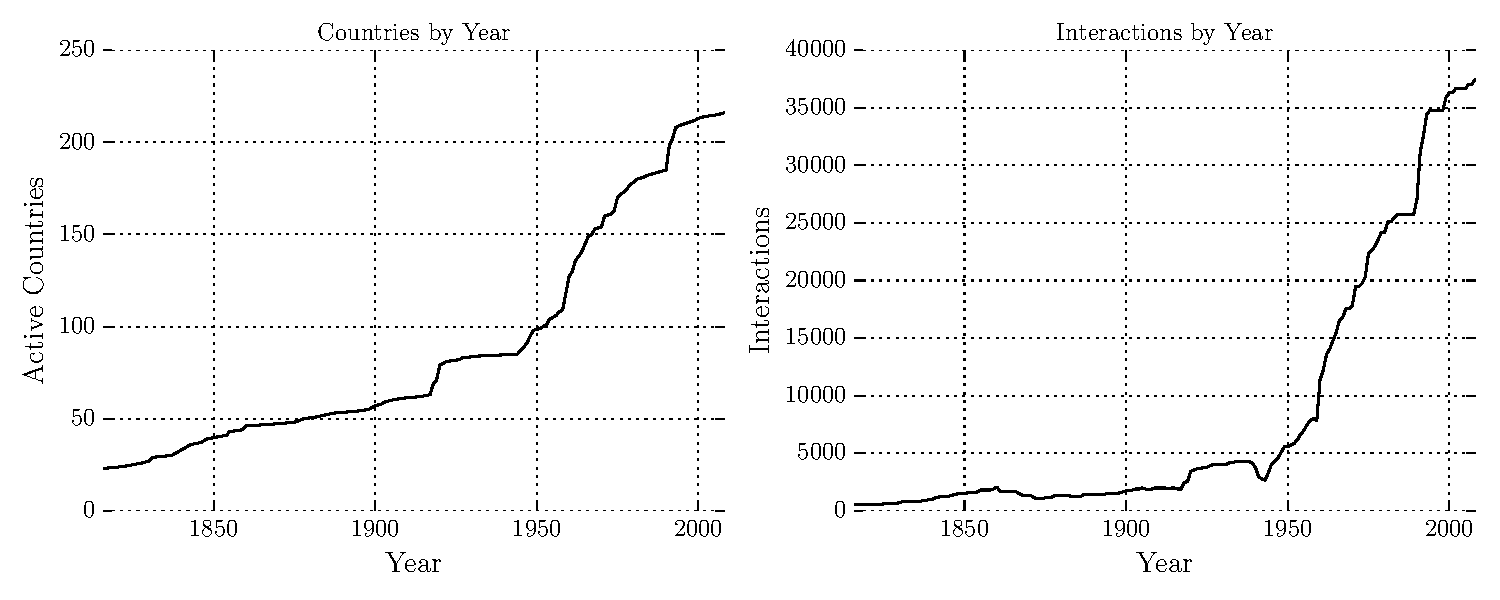
\includegraphics[width=\textwidth]{WarReason/Figures/DataByYear}
    \caption{EUGene Data by Year}
    \label{fig:data_by_year}
    \figSpace
\end{figure}


This methodology allows us to run an agent-based model against historic data. Each agent interaction within each model instantiation corresponding to a particular observed or potential interaction, and the outcome of the model interaction can be compared to the event observed for that interaction. Importantly, as agents only are influenced by their previous interactions, each model outcome is an out-of-sample prediction.

\section{Decisionmaking Models} \label{decisionmaking_models}

Agents in the two models described above have different properties and interact with each other via different games. Over the course of the interactions themselves, however, the agents face the same structure of an extensive-form game, where they must choose one of several moves at each node, with a final payoff depending on the moves both they and their counterpart have made. In most applications of game theory, this model is implicitly perfect rationality; in practice, the equilibrium is found not by agents but by the external modeler (with the so-called gods'-eye view of the situation). The architecture of the agent-based framework I have developed and described here requires an agent-level implementation of any decision rule, including rationality. Any such implementation operationalizes a theory or set of theories of actor decisionmaking.

The framework I describe here makes a few high-level assumptions as to the agent decisionmaking models. The agents have access to the current node of the game, and know all the possible actions they may take at that node. The rational agents described below have access to the full game tree, including the various node payoffs. I also assume that all interactions within a given model implementation share the same game tree structure. Finally, agents do not have direct access to the decisionmaking model of the other agent.

In this section, I describe the three decisionmaking models I implement. The first is classic rationality with perfect information, which serves as a baseline. The second and third are simple reinforcement learning, and a case-based learning extension; both use an experience-weighted attraction implementation so that the actual decisions are stochastic, and vary based on how the attraction weights associated with each move are chosen and updated. In the Reinforcement Learning (RL) decision model, the agents maintain a single set of attraction weights, which they use for all interactions. In the Case-Based Learning (CB) decision model, agents maintain a library of weights learned from past cases, and for each interaction select the weights associated with the most similar past case.

In the next section (Section \ref{experiments-and-results}) I apply these decision models to the Small Crisis Model and International Interaction Game, described above. My initial hypotheses are that, as suggested by previous work on reinforcement learning \citep[e.g.][]{laslier_2005,akramizadeh_2009,galla_2013}, both the RL and CB models will converge to producing outcomes equal to the rational model's (the equilibrium outcomes) more often than we would expect purely at random; I also expect the CB model to outperform the RL model and result in more common equilibrium outcomes, since it adds a degree of coarse-grained strategic reasoning, with agents adjusting their behavior based on their counterpart in each interaction -- implicitly anticipating that agent's own decisions.

\subsection{Rational Model}\label{original-spe-model}

Before implementing additional model variants, I start by reproducing the original rational decisionmaking model. Rational agents have full access to the game tree, and both agents' utilities at each terminal node. They identify the subgame-perfect equilibrium by backwards induction \citep{russell_2009}, finding the correct moves for both players to make at each node and propagating the corresponding utilities up the tree. This leads to a best-response move at all nodes of the tree, not just those that are on the main equilibrium line; thus, even when playing against an opponent who is not playing the equilibrium moves, this agent will be able to choose the game-theoretic best response. In the remainder of this chapter, the equilibrium of an interaction is defined as the result of the interaction when played between two such rational agents.

\subsection{Weighted-Attraction Agents}\label{weighted-attraction-agents}

The game-theoretic model of rationality described above is not time dependent: the particular history of the agent does not matter; the agents, already perfectly rational, do not learn. Furthermore, the agents' decisions are wholly deterministic. Finally, the agents have full awareness of where they are in the game tree, and are capable of planning ahead to the end of the tree, see the plan through, and costlessly replan if the other agent deviates from their expectations.

The two decisionmaking models that follow all begin from different assumptions. In describing the organizational model of decisionmaking, \citet{allison_1999} note that, contrary to the rational model's assumption of perfect lookahead, ``[o]rganizations exhibit great reluctance to base actions on estimates of an uncertain future,'' and instead prefer to utilize existing procedures. As \citet{levy_1986} describes, military organizations in particular tend to prepare plans and procedures which may be inflexibly put into practice in crisis situations. Organizations in general, as \citet{lundberg_1995} reviews, tend to learn in the form of adopting new routines based on past experiences. Finally, \citet{march_1993} note that organizations do not necessarily seek the optimal course of action, and often satisfice -- find a course of action which meets some threshold of acceptability. I distill these characteristics into the following assumptions:

\begin{itemize}
 	\item The agents play the game myopically, choosing each move without explicit look-ahead in the game tree.
 	 \item The agents' choice of move at each node is based on their past experience.
 	 \item At the end of each interaction, the agents only have knowledge of the actual outcome, and cannot directly compare it to the `road not taken.' 
 \end{itemize}

These assumptions are implemented via experience-weighted attraction (EWA), a particular form of reinforcement learning \citep{sutton_1998,galla_2013}. At each node of the game tree, agents associate a certain weight with each potential action they can take. They choose among the actions stochastically, in proportion to the weight they place on each. If the weights are equal, all actions may be chosen with equal probability; if one action has overwhelmingly more weight than the others, it will be chosen with probability approaching 1. These weights are learned based on the agent's past experiences, and in particular the utilities they gained at the end of previous interactions. The specific ways the weights are learned are explained in the subsections below. 

This model form is taken proximately from \citet{galla_2013}, who in turn adopt it from several other sources \citep{camerer_2002,kocher_2005,ho_2007}. Most importantly for our purposes, the experimental results reported by \citet{kocher_2005} indicate that EWA is an effective model for strategic learning not just by individuals but by groups tasked with making a decision jointly.

Formally, the model is as follows. Within a particular interaction, an agent $i$ has an attraction function $ Q_i : s_{x,k} \mapsto w$ which maps from $s_{x,k}$, a move available at node $x$, to a numeric weight $w$. In practice, this is implemented as an associative array, with node-move tuples as keys and weights as values. At node $x$, the agent chooses move $s_{x,k}$ with probability:

\begin{equation}
    P_i(s_{x,k}) = \frac{exp(\beta Q_i(s_{x,k}))}{\sum_{s_{x,m}}exp(\beta Q_i({s_{x,m}}))}
\end{equation}

Where $\beta$ is a fixed parameter which further weights the choice weights. When $\beta=0$, all moves are equally likely regardless of weight. The larger $\beta$ is, the more likely a move with a smaller weight advantage is to be chosen. In general, I set $\beta=1$ for all agents; however, as this is an agent-level parameter, there is nothing preventing agents from having heterogeneous $\beta$ values.

In Python-style pseudocode, the agent class's EWA method is implemented as follows:

\begin{singlespace}
\begin{lstlisting}[language=python,caption={Experience-Weighted Attraction},label={code:ewa}]
def step(model):
    current_state = model.current_node
    choices = {}
    for move in model.tree[current_state].children:
        choices[move] = self.Q[key]
    choice = self.weighted_choice(choices, self.beta)
    self.past_moves.append((current_state, choice))
    return choice
\end{lstlisting}
\end{singlespace}

This decision framework can be thought of in several ways. It can simply represent the relevant decisionmakers' view of the relative merit of each possible course of action \citep{kocher_2005}. It can also represent the relative influence or credibility of different factions or sub-actors advocating for different courses of action, or standing procedures developed by the relevant organizations, such as reserve call-ups or troop movements \citep{levy_1986}. How to interpret it will rest partially on the particular learning rule, which will determine how the weights are learned and updated between interactions. The two learning rules I use are described next.

\subsection{Pure Reinforcement Learning}\label{pure-reinforcement-learning}

This model variant is the closest to traditional EWA, as described in \citet{galla_2013} and elsewhere. Under this decisionmaking model, agents choose actions based on their total past experiences, without taking into account any of the properties of the specific agent they are interacting with, or the broader environment. At the end of every interaction, agents update their attraction to each move they made based on the payoff they received. Moves which led to higher utilities will be more likely to be played again, while ones that led to lower utilities (and in particular, to negative utilities) will be less likely to be played again.

In terms of crisis behavior, this variant can be thought of as a stylized version of the organizational procedure model described by \citet{allison_1999}. The agents are developing `standard operating procedures' they will follow without evaluating their appropriateness for the particular crisis they are facing at the moment. When the crisis is resolved, they will update their procedures based on the crisis's outcomes. To be sure, this is an exaggerated view of the organization procedure model, as nobody claims that states act solely on the basis of preset, inflexible procedures. Yet if so, it may also be no more exaggerated than the game-theoretic operationalization of the rational choice model.

Formally, each agent has a single experience table $Q_i$, encoding the utility it has gained from making decisions at each node in the past. This experience table drives the decisionmaking at each node of the game tree, until the interaction ends. At that point, the table is updated at the end of the interaction with the corresponding utility.

At the end of an interaction, let the set of moves agent $i$ has decided to play be $S_i = \{ s_{x_0,k}... s_{x_l,k} \}$ for each node in the game tree. Let $\Pi _i$ be the payoff associated with the terminal node reached by $S_i$ and $S_j$. The updating rule is then:

\begin{equation}
    Q^{t+1}_i(s_{x,k} \in S_i) = \alpha \Pi _i +  (1-\alpha) Q^{t}_i(s_{x,k}) 
\end{equation}

Parameter $\alpha$ is the learning rate, where $\alpha \in {[0, 1]}$. When $\alpha=1$, the agent has effectively no memory, and associates a move only with its most recent payoff. Conversely, if $\alpha=0$ the agent never updates its attraction weights. In practice, obviously, this value will be somewhere in between these extremes. The $\alpha$ value is set by the modeler; I will explore its effects in Section \ref{small_crisis_results}.

This model differs from some other, similar models, in that it attempts to capture realistic learning from experience rather than serve as an optimization algorithm. Thus, it does not incorporate fictitious play \citep{shoham_2003}, and agents have no ability to access other potential payoffs from decisions not taken. Importantly, due to this, the weights on moves not taken do not update, meaning that entire branches of the game tree may be unaffected by a particular interaction where play does not pass through that branch. Similarly, the weight on any move not taken is not updated; thus, whether a particular update will substantially change the probability of a move being chosen in the future depends not just on the move's own updated weight, but the weight present on the moves not chosen.

In Python-style pseudocode, the agent's experience update method is provided below. Note that this uses the \emph{past\_moves} list updated in Code Block \ref{code:ewa}.

\begin{singlespace}
\begin{lstlisting}[language=python,caption={Reinforcement Learning},label={code:rl_update}]
def add_utility(utility):
    for move in self.past_moves:
        self.Q[move] *= (1 - self.learning_rate)
        self.Q[move] += self.learning_rate * utility
\end{lstlisting}
\end{singlespace}

\subsection{Case-Based Learner}\label{case-based-learner}

In the previous model variant, agents' past experiences were undifferentiated: the agents maintain and update a single experience table across all their interactions. This means that in a new interaction, the agent will utilize the same decision weights whether facing, for example, a strong ally or a weak rival. However, individuals and organizations are capable of maintaining and recalling and utilizing discrete memories of specific circumstances they have previously encountered. \citet{gilboa_1995} argue that case-based reasoning provides a cognitively plausible model of how individuals reason under uncertainty; similarly, \citet{march_1993} describe one of the modes of organizational decisionmaking as choosing actions based on recognizing a given situation's similarity to previously-encountered ones stored in organizational or individual memory, and retrieving rules associated with those situations. In the context of international crises and conflicts, the relevant situations are most often prior crises and conflicts. Historic analogies help shape decisionmakers' view of the stakes of a crisis, as well as the probabilities and risks associated with various courses of action \citep{khong_1992}. These analogies influence the public debate surrounding potential conflicts \citep{schuman_1992,noon_2004,schuman_2006}, as well as the strategies and tactics which may be brought to bear (e.g. \citealt{nagl_2002} and too many military `Lessons Learned' to cite). Furthermore, lessons learned from some conflicts may also lead to the reevaluation of previous conflicts (e.g. \citealt{hagerman_1992} or \citealt{forster_2002}, among many examples), sometimes exaggerated to lead to thought experiments such as a reevaluation of the American Revolutionary War in light of the lessons of the United States's Iraq and Afghanistan wars \citep{exum_2008}.

In order to model such reasoning by historic analogy, I extend the reinforcement learning model into a case-based decisionmaking model \citep{ram_1997,mantaras_2001,jiang_2009}. Instead of each agent having a single experience table, they now possess a library of such tables representing previous interactions (the cases), indexed by key salient features of each case. At the beginning of each interaction, the agents query their case library for the experience table associated with the most similar case, and use it to drive their decisionmaking for this interaction -- in other words, when facing a new case, agents approach it based on the lessons learned from the most similar previous case they have faced. At the end of the interaction, this previous table is updated, and a copy of the updated table is added to the case library, indexed at the coordinates of the current case. Thus, the lessons learned from the current case are propagated back to the previous case as well. The more frequently a case is the most-similar one, the more information (encoded as move weights) the agent has about it. This captures the fact that actors' understanding of the past is not static, and is updated based on their further experiences. While the agents in this model variant are still not `strategic' in the game-theoretic sense, they are retrieving different past experiences based on the properties (and hence, expected behavior) of the agent with whom they are currently interacting.

More formally this decisionmaking model is as follows. Let $c_i(j)$ encode a tuple of coordinates describing agent $i$'s interaction with agent $j$. Each agent $i$ has a case library of coordinates and associated attraction functions $C_i = \{(c_{i,0}, Q_{i,0}), (c_{i,1}, Q_{i,1})... \}$. When presented with a new case $c_{new}$, the agent chooses $c_* = argmin_{c \in C_i} dist(c_{new}, c)$ and the corresponding $Q_*$. $Q_*$ becomes the active attraction function for the given interaction, as described above. 

At the end of the interaction, $Q^{t+1}_*$ is updated as described above. The overall case library is then updated such that $c_* \mapsto Q^{t+1}_*$ and $c_{new} \mapsto Q^{t+1}_*$.

This decision model is implemented as follows. At the beginning of each interaction, the agent selects the active case, and corresponding experience table:

\begin{singlespace}
\begin{lstlisting}[language=python,caption={Case-Based Learning -- Set Case},label={code:cb_setccase}]
def set_new_case(coords):
    self.current_coords = coords
    self.current_case = self._get_nearest_neighbor(coords)
    self.Q = self.case_library[self.current_case]
\end{lstlisting}
\end{singlespace}

At the end of the interaction, the case library is then updated as follows:

\begin{singlespace}
\begin{lstlisting}[language=python,caption={Case-Based Learning -- Update Weights},label={code:cb_update}]
def add_utility(utility):
    for move in self.past_moves:
        self.Q[move] *= (1 - self.learning_rate)
        self.Q[move] += self.learning_rate * utility
    self.past_moves = []
    new_Q = self.Q.copy()
    self.case_library[self.current_coords] = new_Q
\end{lstlisting}
\end{singlespace}

The coordinates used for the cases are as follows:

\begin{description}
	\item[Small Crisis Model:] \begin{equation}
	c_i(j) \equiv (\Delta m, \Delta a, 100\delta(b_i,b_j))
	\end{equation}
	where $\Delta m = m_i - m_j$ and likewise for $\Delta a$, and $\delta(b_i,b_j)=1$ if $b_i=b_j$, and $0$ otherwise.
	\item[International Interaction Game:]\begin{equation}
	c_i(j) \equiv (Stakes_i, Stakes_j, P^i)
	\end{equation}
	Where $Stakes_i$ is defined in \citet{bdm_1992} as $U^i(\Delta_i) - U^i(\Delta_j)$ (see Equations \ref{eq:u_a1} and \ref{eq:u_a2}), and $P^i$ is defined in Equation \ref{eq:prob_win}.
\end{description}

\section{Experiments and Results}\label{experiments-and-results}

We now have all the necessary components in hand: two models of agent interaction, and two new models of agent decisionmaking in addition to the baseline rational model. Now we can combine them and observe the results. I first test the Reinforcement Learning (RL) and Case-Based (CB) agent decisionmaking models with the Small Crisis Model and compare their performance to one another and to the game-theoretic equilibrium. I next apply the RL and CB models to the full International Interaction Game and the EUGene data, analyze the models' behavior against both the equilibrium outcomes and the observed events, and test the model outputs' power as predictive variables. 

\subsection{Small Crisis Model} \label{small_crisis_results}
 
Before we apply the decisionmaking models to historic data, it is worthwhile to test them in a simpler, notional environment. This allowed me to test and verify the decisionmaking models themselves; as the decision trees are relatively small, and the payoff calculations straightforward, it allowed me to manually verify that the decisionmaking code matched the model descriptions, and was behaving as expected. Furthermore, this model provides a baseline against which to judge the decisionmaking models' performance. If agents in the notional system, when using decision models other than game-theoretic rationality, behave very differently from the equilibrium expectation, this leads us to hypothesize that a similar divergence should exist in reality. If, however, the agents' behavior converges to something similar to the equilibrium, it would make the real-world decision models harder to distinguish, but potentially provide support for the use of the equilibrium model -- as an approximation of state behavior rather than a direct description of it.

I carry out the experiments as follows. I instantiate Small Crisis models of 10 agents, as described in Section \ref{small_crisis}: first using the Static variants, then Dynamic one. For both model variants, I vary the learning rate $\alpha$ from 0.1 to 1, in increments of 0.1. At each parameter value, I generate 100 model instantiations. Each instantiation is done using a fixed random seed, and generates two model runs: one with agents utilizing the Reinforcement Learning (RL) decisionmaking model, and one with the Case-Based Learning (CB) decisionmaking model. Using the same random seed ensures that the random elements are fixed between the model runs -- in particular, that the agent properties are the same\footnote{In some cases, individual interactions between agents result in different-length paths through the game tree, which will lead to a divergence in the sequence of random numbers.}. The models are instantiated with agents with the same properties; these agents will interact in the same order; even the random numbers drawn when agents choose between moves will be the same. 

For each model run, I record the outcome of each interaction, as well as the equilibrium outcome for that interaction. In particular, I focus on the fraction of interactions within every simulated year where the interaction outcome matches the equilibrium outcome. I also define run quality as the mean of those fractions over the latter 50 steps of each run; this allows for a burn-in period as the agents gain initial information, discarding the early interactions where the agents' moves are approximately random. This metric allows for comparison between the behavior of the learning models and the rational model, and specifically measures the correspondence between them.

I begin with several hypotheses: first, as mentioned in Section \ref{decisionmaking_models}, that across both the Static and Dynamic variants, both the RL and CB agents will converge to near-equilibrium behavior -- that is, they will learn to play similarly to agents utilizing the purely rational decisionmaking model. I further expect that the CB agents will exhibit higher run quality (as defined above), since it allows agents to incorporate additional information and learn different weights -- that is, different likely moves -- for different interactions, implicitly incorporating a greater degree of strategic anticipation of the other agent's moves. Finally, in the Static variant, the mix of equilibria for each agent, and the equilibrium of each agent dyad, are fixed for the duration of each run, giving the agents more time to converge on the corresponding moves; in contrast, in the Dynamic variant these equilibria may change, meaning that the move weights learned from prior interactions may no longer be as likely to reach each interaction's equilibrium. Thus, I expect both the CB and RL decisionmaking models to perform worse in the Dynamic variant than in the Static one.
%% NOTE: Following paragraphs are discussing Static World Ex3, and Dynamic World Ex5.

\subsubsection{Static Variant}

\begin{figure}[h!]
	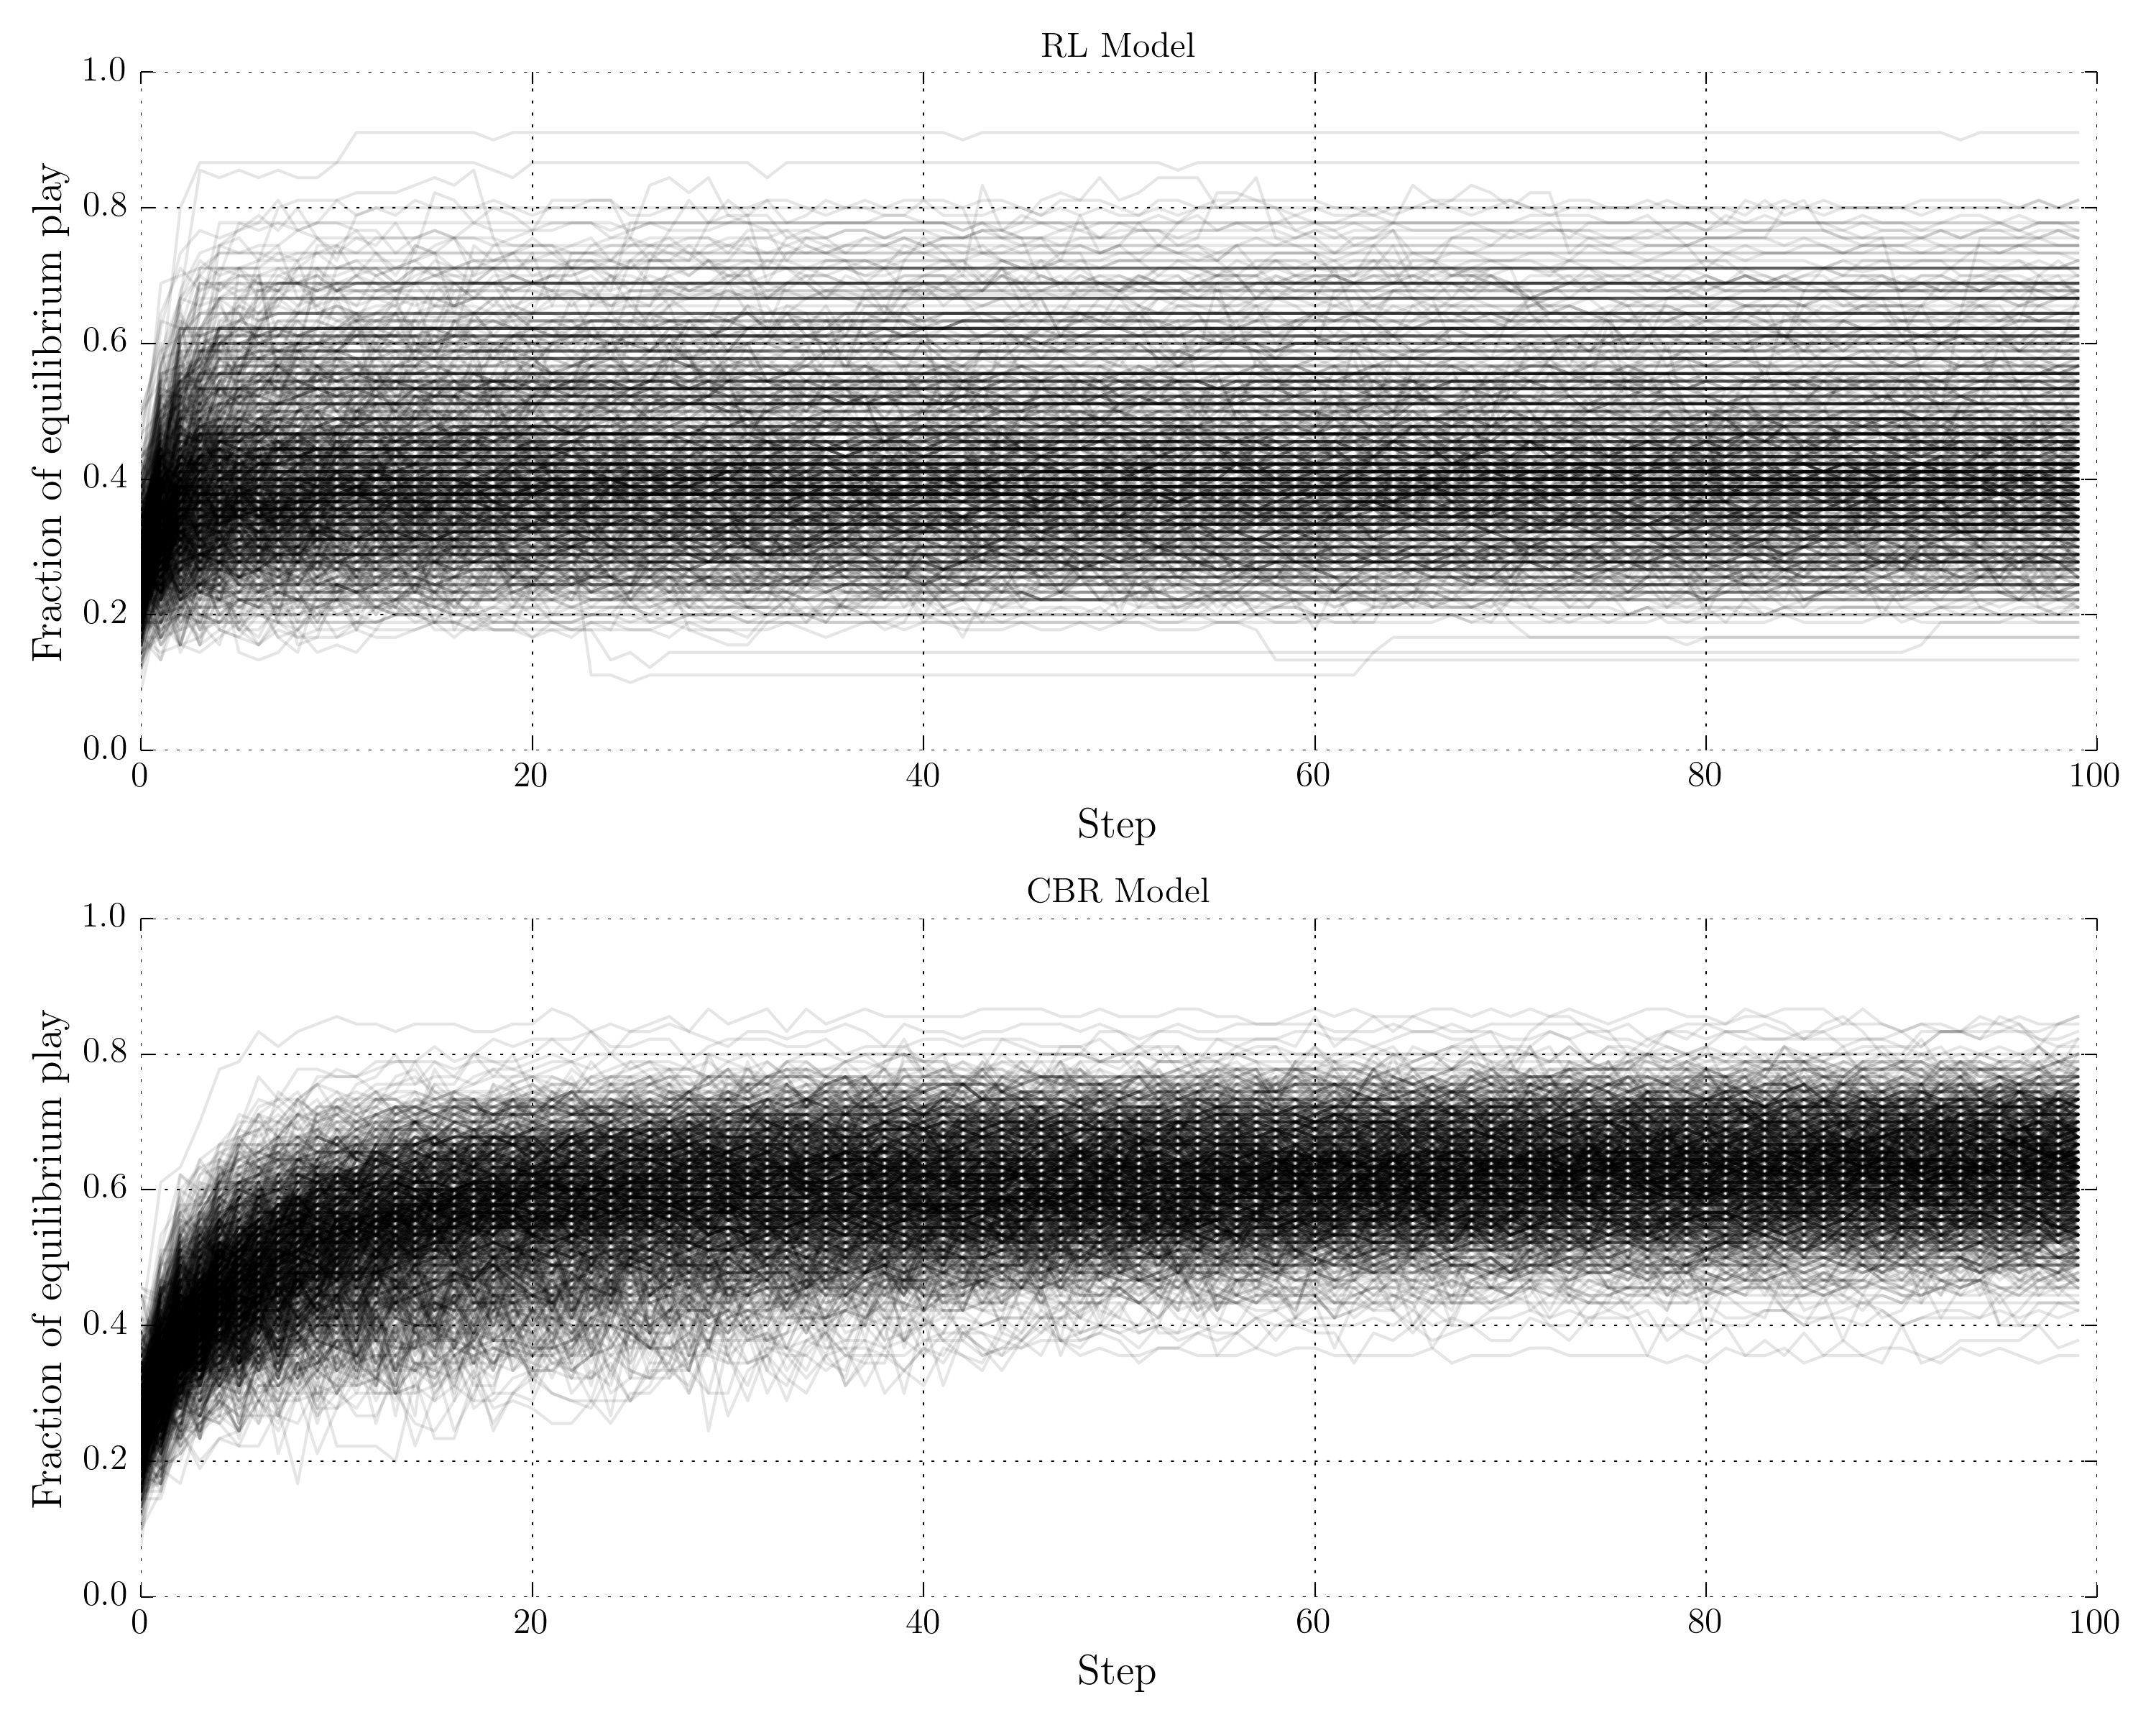
\includegraphics[width=\textwidth]{WarReason/Figures/SC_1_traces}
    \caption{Small Crisis (Static) -- Traces}
    \label{fig:sc1_traces}
    \figSpace
\end{figure}

\begin{figure}[h!]
	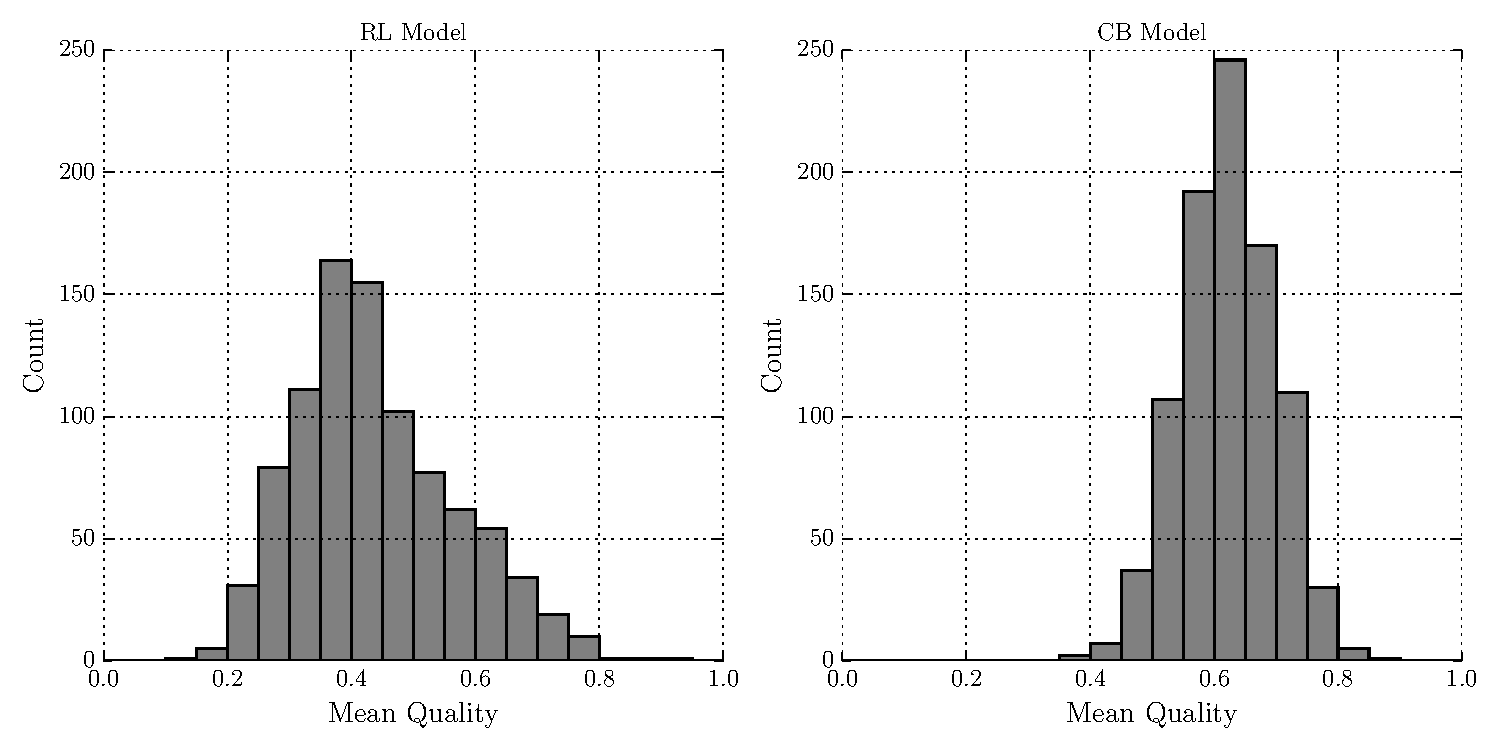
\includegraphics[width=\textwidth]{WarReason/Figures/SC_1_histograms}
    \caption{Small Crisis (Static) -- Quality Distribution}
    \label{fig:sc1_outcomes}
    \figSpace
\end{figure}

\begin{figure}[h!]
	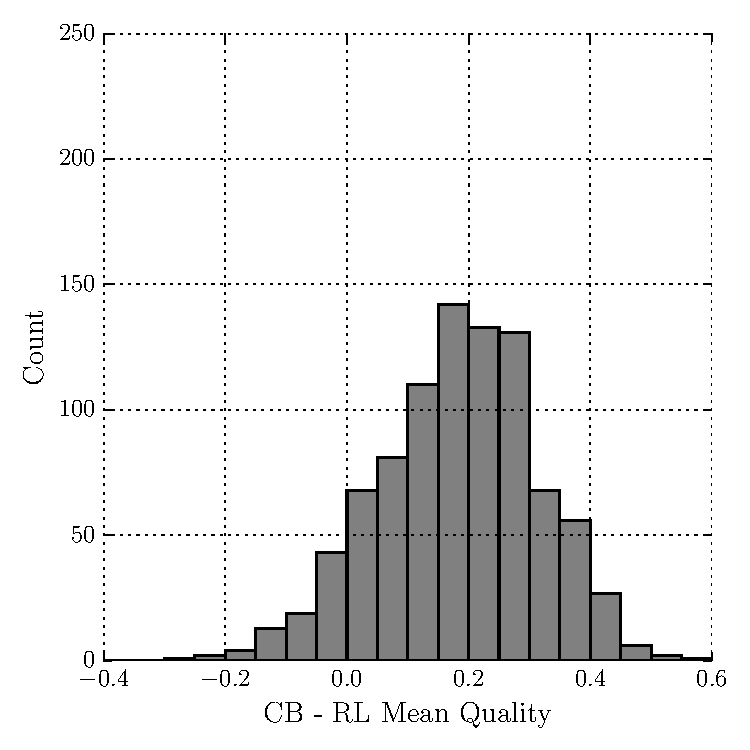
\includegraphics[width=0.5\textwidth]{WarReason/Figures/SC_1_deltas}
    \caption{Small Crisis (Static) -- CB and RL Differences}
    \label{fig:sc1_deltas}
    \figSpace
\end{figure}


Initially, let us examine the Static variant runs. Figure \ref{fig:sc1_traces} shows the traces of the equilibrium frequency at each step across all the model runs, for both agent types. For the pure RL agents, we see a variety of behaviors emerging: in some cases, the models rapidly converge to near-equilibrium behavior, while in others appear to converge to a behaviors further away from equilibrium than we would expect solely due to chance. Figure \ref{fig:sc1_outcomes} shows the distributions of the run qualities (mean fraction of interactions where the outcome matches the equilibrium) across the different runs. We immediately see that both distributions are skew normal. The CB model produces better (more consistently closer to equilibrium) behavior: its mean is greater, while its standard deviation and skew are both smaller. This is in line with my earlier hypothesis in Section \ref{decisionmaking_models}, and implies that the CB model provides agents with more strategic behavior.

Since each model instantiation is run twice with the same seed, once with RL agents and once with CB agents, we can directly compare the equilibrium frequency for each seed and find the difference between the CB and RL mean equilibrium frequencies for each. The distribution of the differences is shown in Figure \ref{fig:sc1_deltas}. This distribution is also approximately skew normal, with a mean of 0.18 ($p$-value indistinguishable from 0). This allows us to conclude that the case-based learning decisionmaking model produces behavior which is robustly better than the pure reinforcement learners when controlling for other factors -- exactly as we would expect.
%% RAX: Normality test?

\begin{figure}[h!]
	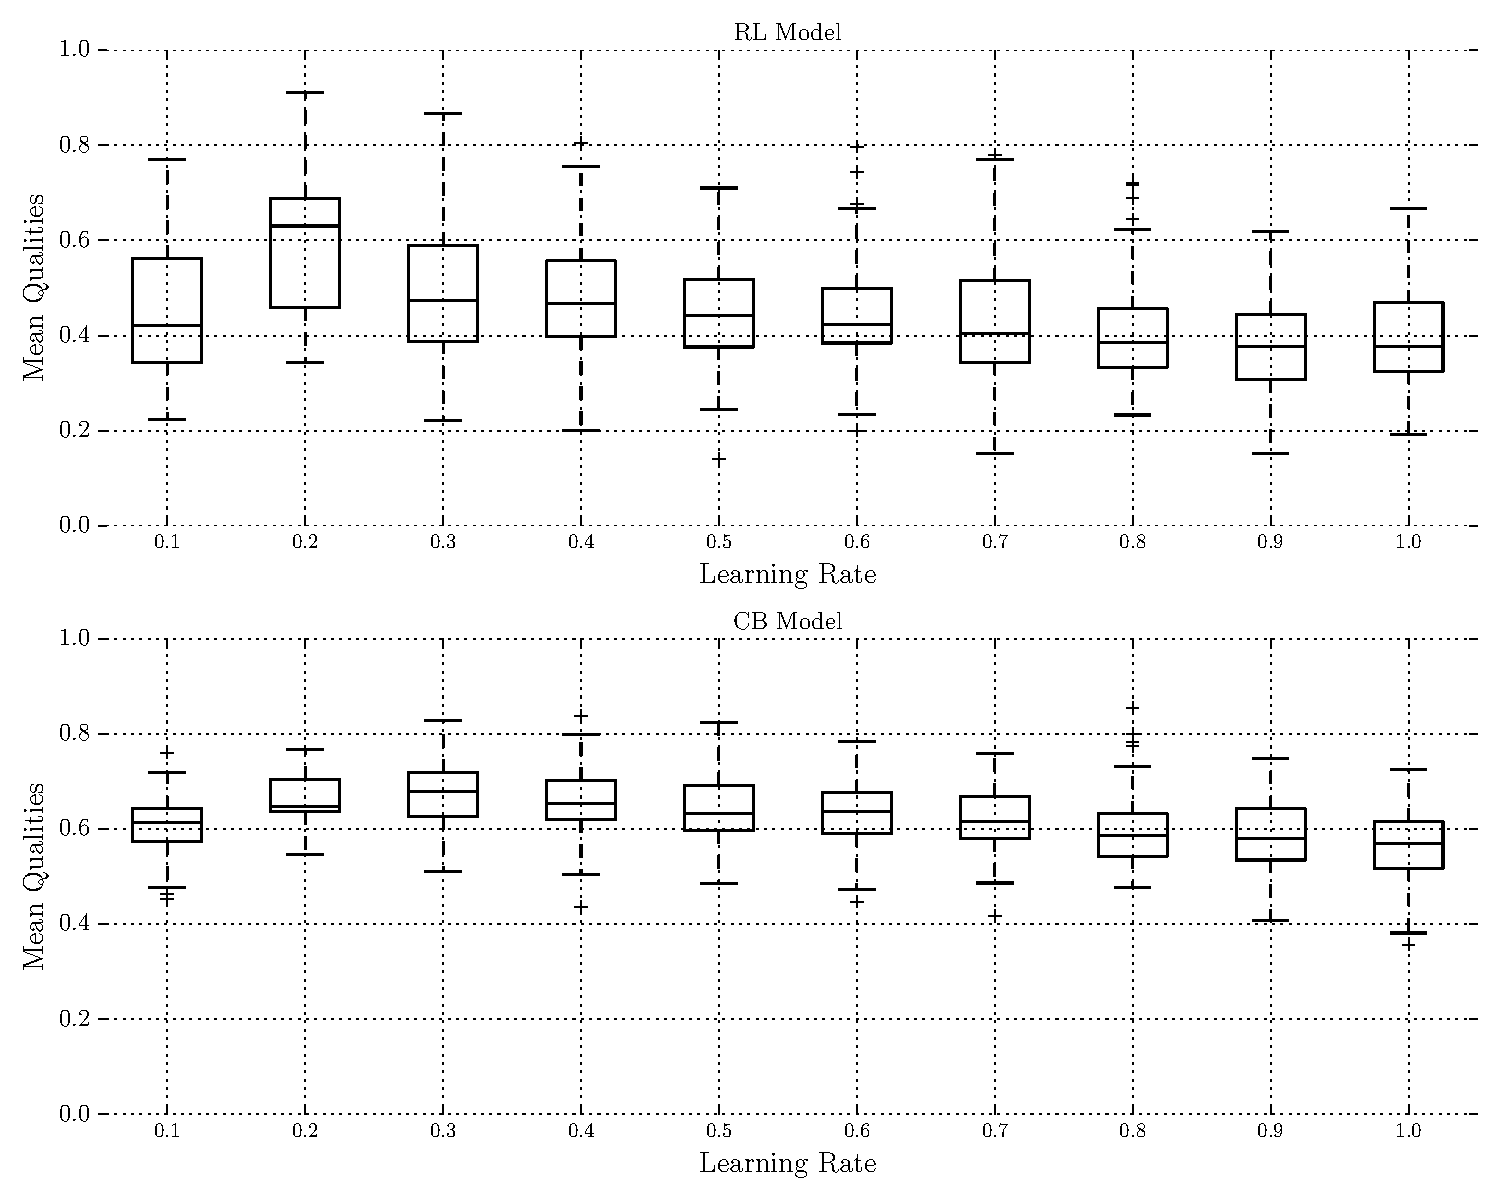
\includegraphics[width=\textwidth]{WarReason/Figures/SC_1_boxwhiskers}
    \caption{Small Crisis (Static) -- Quality by Learning Rate}
    \label{fig:sc1_boxwhiskers}
    \figSpace
\end{figure}

Another important question is whether different learning parameters yield substantially different behaviors. Figure \ref{fig:sc1_boxwhiskers} shows box-and-whiskers plots comparing the distribution of run qualities for each learning rate parameter. Overall, the differences are small, though statistically significant (with one- and two-way ANOVA tests yielding $p$-values indistinguishable from zero). Linear models of run quality to learning rate place a negative coefficient on the learning rate, indicating that lower learning rates tend to lead to higher expected qualities\footnote{Note, however, that there is a discontinuity at $\alpha=0$ where the initial weights would never change, meaning that all decisions will be made with equal probability.}. In other words, agents learn best when adjusting their behavior relatively slowly and placing most of the weight on the total of their past experiences rather than each new one -- again, an intuitive but satisfying result. Visual examination of the results in Figure \ref{fig:sc1_boxwhiskers} suggests that performance does not have a simple linear relationship with learning rate, and that both decisionmaking models have an optimal learning rate, which are different for each. The median quality for the RL model where the learning rate is 0.2 is substantially higher than the maximum of the inter-quartile range (the box) for the rest of the values, indicating that the maximum performance is attained somewhere near $\alpha \approx 0.2$. There is no similar obvious optimal learning rate for the CB model; a learning rate of 0.3 produces the highest median quality, but the distributions produced by values between 0.3 and 0.5 are essentially indistinguishable from one another, though higher than the distributions produced at the extreme values.
% RAX: Can we compare to other models w/ adjustable learning constants?

Even the best-performing model runs do not result in equilibrium play on all interactions; in general, the majority of model instantiations see equilibrium outcomes on the order of half the interactions. However, as we will discuss in more detail below, the majority of historic real-world interactions do not result in the equilibrium either. Suppose that the decisionmaking process of the model agents were an unknown black box, as real states' decisionmaking processes are. We could propose the game-theoretic equilibrium as a model of the agent decisionmaking, and test whether the equilibrium outcome is a useful predictor of the interaction outcomes. Following the methodology of \citet{bennett_2000}, I use logistic regressions to test whether the equilibrium is indeed a good predictor of observed outcomes.

\begin{table}
	\caption{Small Crisis (Static) -- Logistic Regressions}
	\label{table:sc1_logits}
	\begin{subtable}{\textwidth}
	\begin{center}
	\caption{RL Model}
	\begin{tabular}{lccccc}
		\hline
		            & StatusQuo & Capitulate1 & Capitulate2 &   War1   &   War2     \\
		\hline
		Capitulate1 & -0.04***  & 2.73***     & 0.76***     & -1.49*** & 1.19***    \\
		            & (0.00)    & (0.01)      & (0.01)      & (0.01)   & (0.01)     \\
		Capitulate2 & -0.42***  & 1.79***     & 1.43***     & -0.93*** & -0.99***   \\
		            & (0.00)    & (0.01)      & (0.00)      & (0.01)   & (0.02)     \\
		War1        & -0.08***  & -0.52***    & -0.41***    & 0.13***  & 1.30***    \\
		            & (0.00)    & (0.02)      & (0.00)      & (0.00)   & (0.01)     \\
		Const.      & 1.05***   & -5.63***    & -2.55***    & -1.55*** & -4.79***   \\
		            & (0.00)    & (0.01)      & (0.00)      & (0.00)   & (0.01)     \\
		\hline
		\hline
		\multicolumn{6}{l}{Standard errors in parentheses.} \\
		\multicolumn{6}{l}{* $p<.1$, ** $p<.05$, *** $p<.01$} \\
		\end{tabular}
		\end{center}
		%\label{table:sc1_logits}
		\tableSpace
	\end{subtable}


	\begin{subtable}{\textwidth}
		\begin{center}
		\caption{CB Model}
		\begin{tabular}{lccccc}
					&			&			  &				&		   &           \\
		\hline
		            & StatusQuo & Capitulate1 & Capitulate2 &   War1   &   War2     \\
		\hline
		Capitulate1 & -0.44***  & 4.28***     & 0.70***     & -1.36*** & 1.88***    \\
		            & (0.00)    & (0.01)      & (0.01)      & (0.01)   & (0.01)     \\
		Capitulate2 & -1.08***  & 0.70***     & 3.51***     & -1.98*** & -3.09***   \\
		            & (0.00)    & (0.02)      & (0.00)      & (0.01)   & (0.07)     \\
		War1        & -1.74***  & 0.46***     & -0.36***    & 1.67***  & 0.96***    \\
		            & (0.00)    & (0.01)      & (0.01)      & (0.00)   & (0.01)     \\
		Const.      & 0.48***   & -5.35***    & -3.23***    & -0.70*** & -4.89***   \\
		            & (0.00)    & (0.01)      & (0.00)      & (0.00)   & (0.01)     \\

		\hline
		\hline
		\multicolumn{6}{l}{Standard errors in parentheses.} \\
		\multicolumn{6}{l}{* $p<.1$, ** $p<.05$, *** $p<.01$} \\
		\end{tabular}
		\end{center}
		%\label{table:sc1_logits}
	\end{subtable}
\tableSpace
\end{table}

\begin{figure}[h!]
	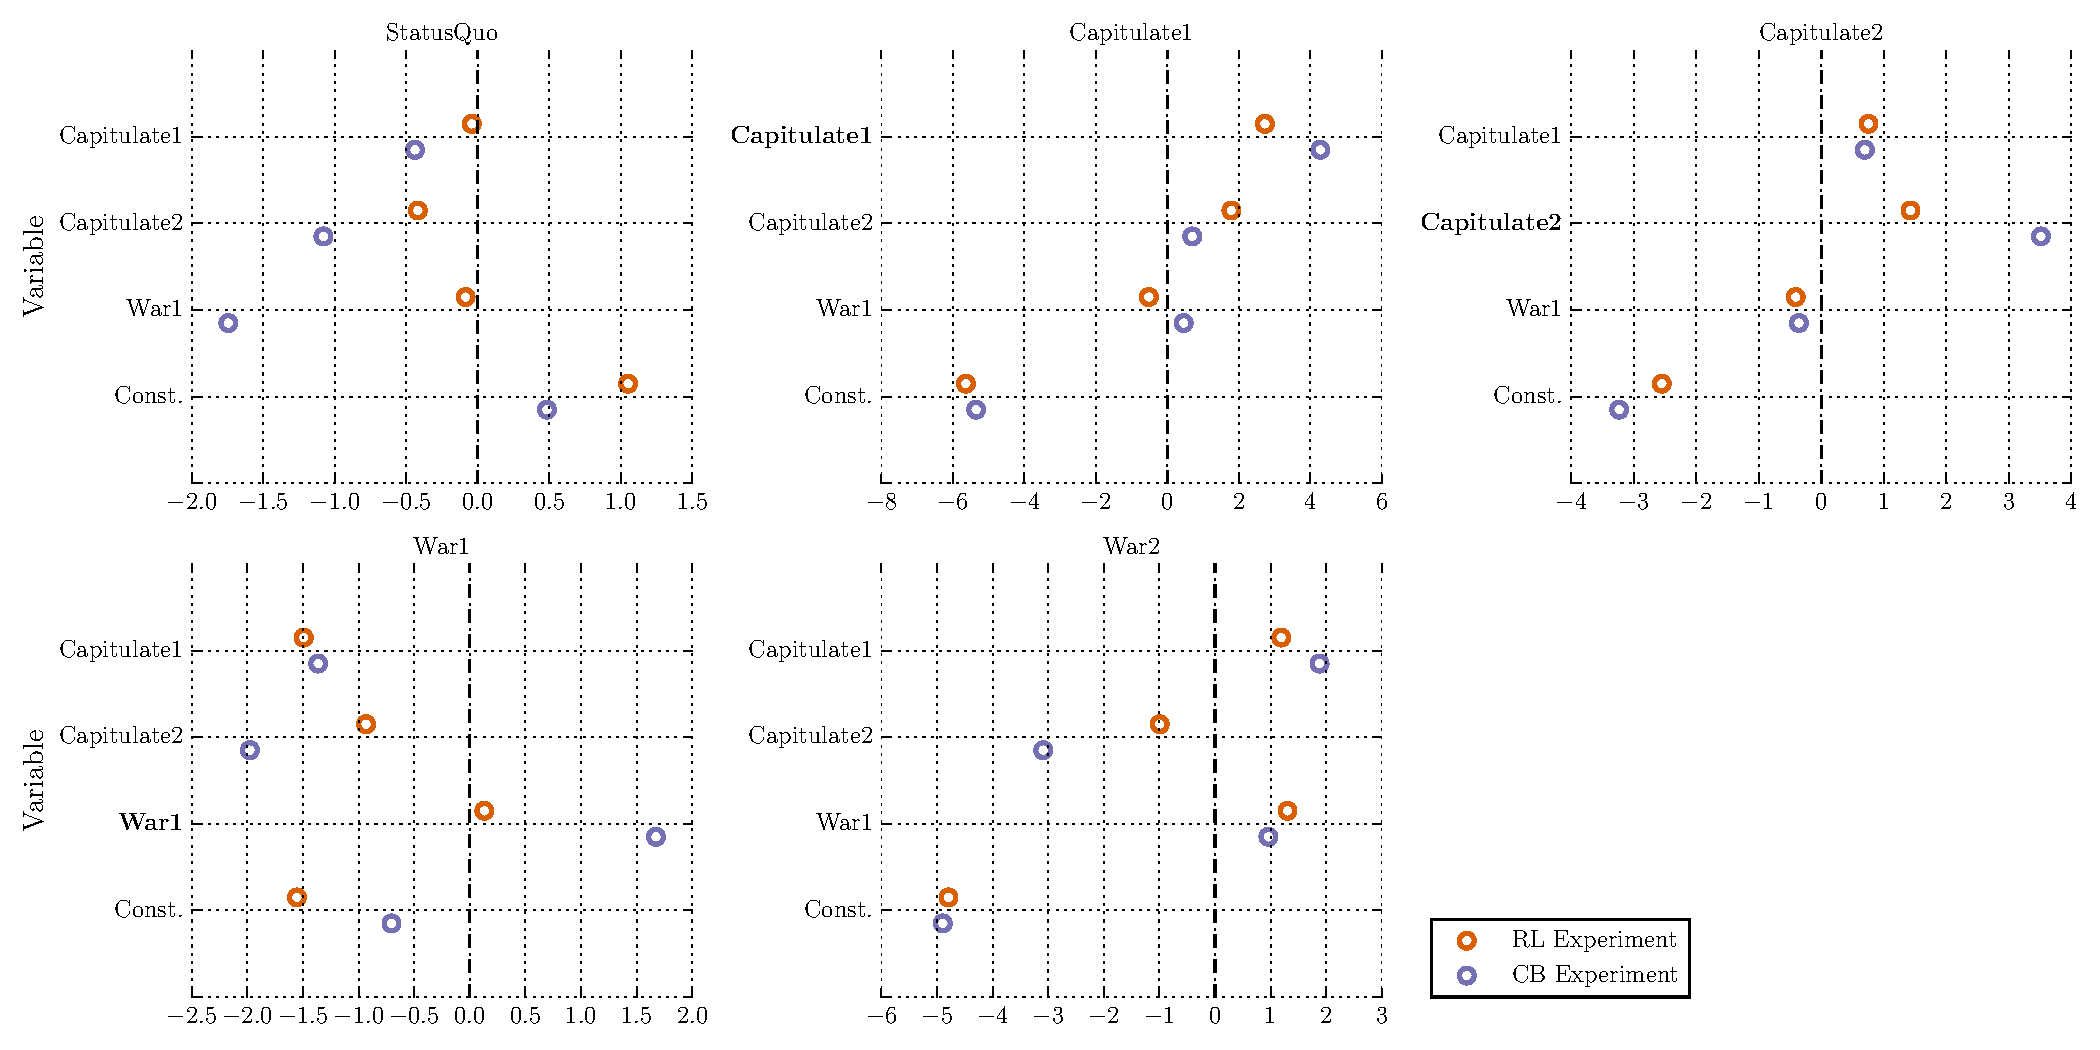
\includegraphics[width=0.95\textwidth]{WarReason/Figures/SC1_Coeffs}
    \caption{Small Crisis (Static) -- Logistic Regression Coefficient Plots}
    \label{fig:sc1_coeffs}
    \figSpace
\end{figure}

The results of these regressions are reported in Table \ref{table:sc1_logits}, and shown visually in Figure \ref{fig:sc1_coeffs}. In line with the results of \citet{bennett_2000}, across both decisionmaking models, the equilibrium is a strong predictor of a corresponding observed outcome, while other equilibria have smaller, often negative, coefficients. This effect is consistently more powerful for the CB model, with larger equilibrium coefficients and smaller coefficients on other variables for each regression. In other words, when the agents are using case-based learning, the equilibria is a stronger predictor of their actual behavior than when the agents are using simple reinforcement learning. This is in line with the hypothesis that the CB agents will behave more rationally than the RL agents. Furthermore, outcomes closer to the equilibrium in the game tree are stronger predictors than further outcomes, suggesting that the agents are playing sequences of moves that are close to the equilibria sequences, deviating only in the step.  
% Last point seems important -- expand?

\begin{figure}[h!]
	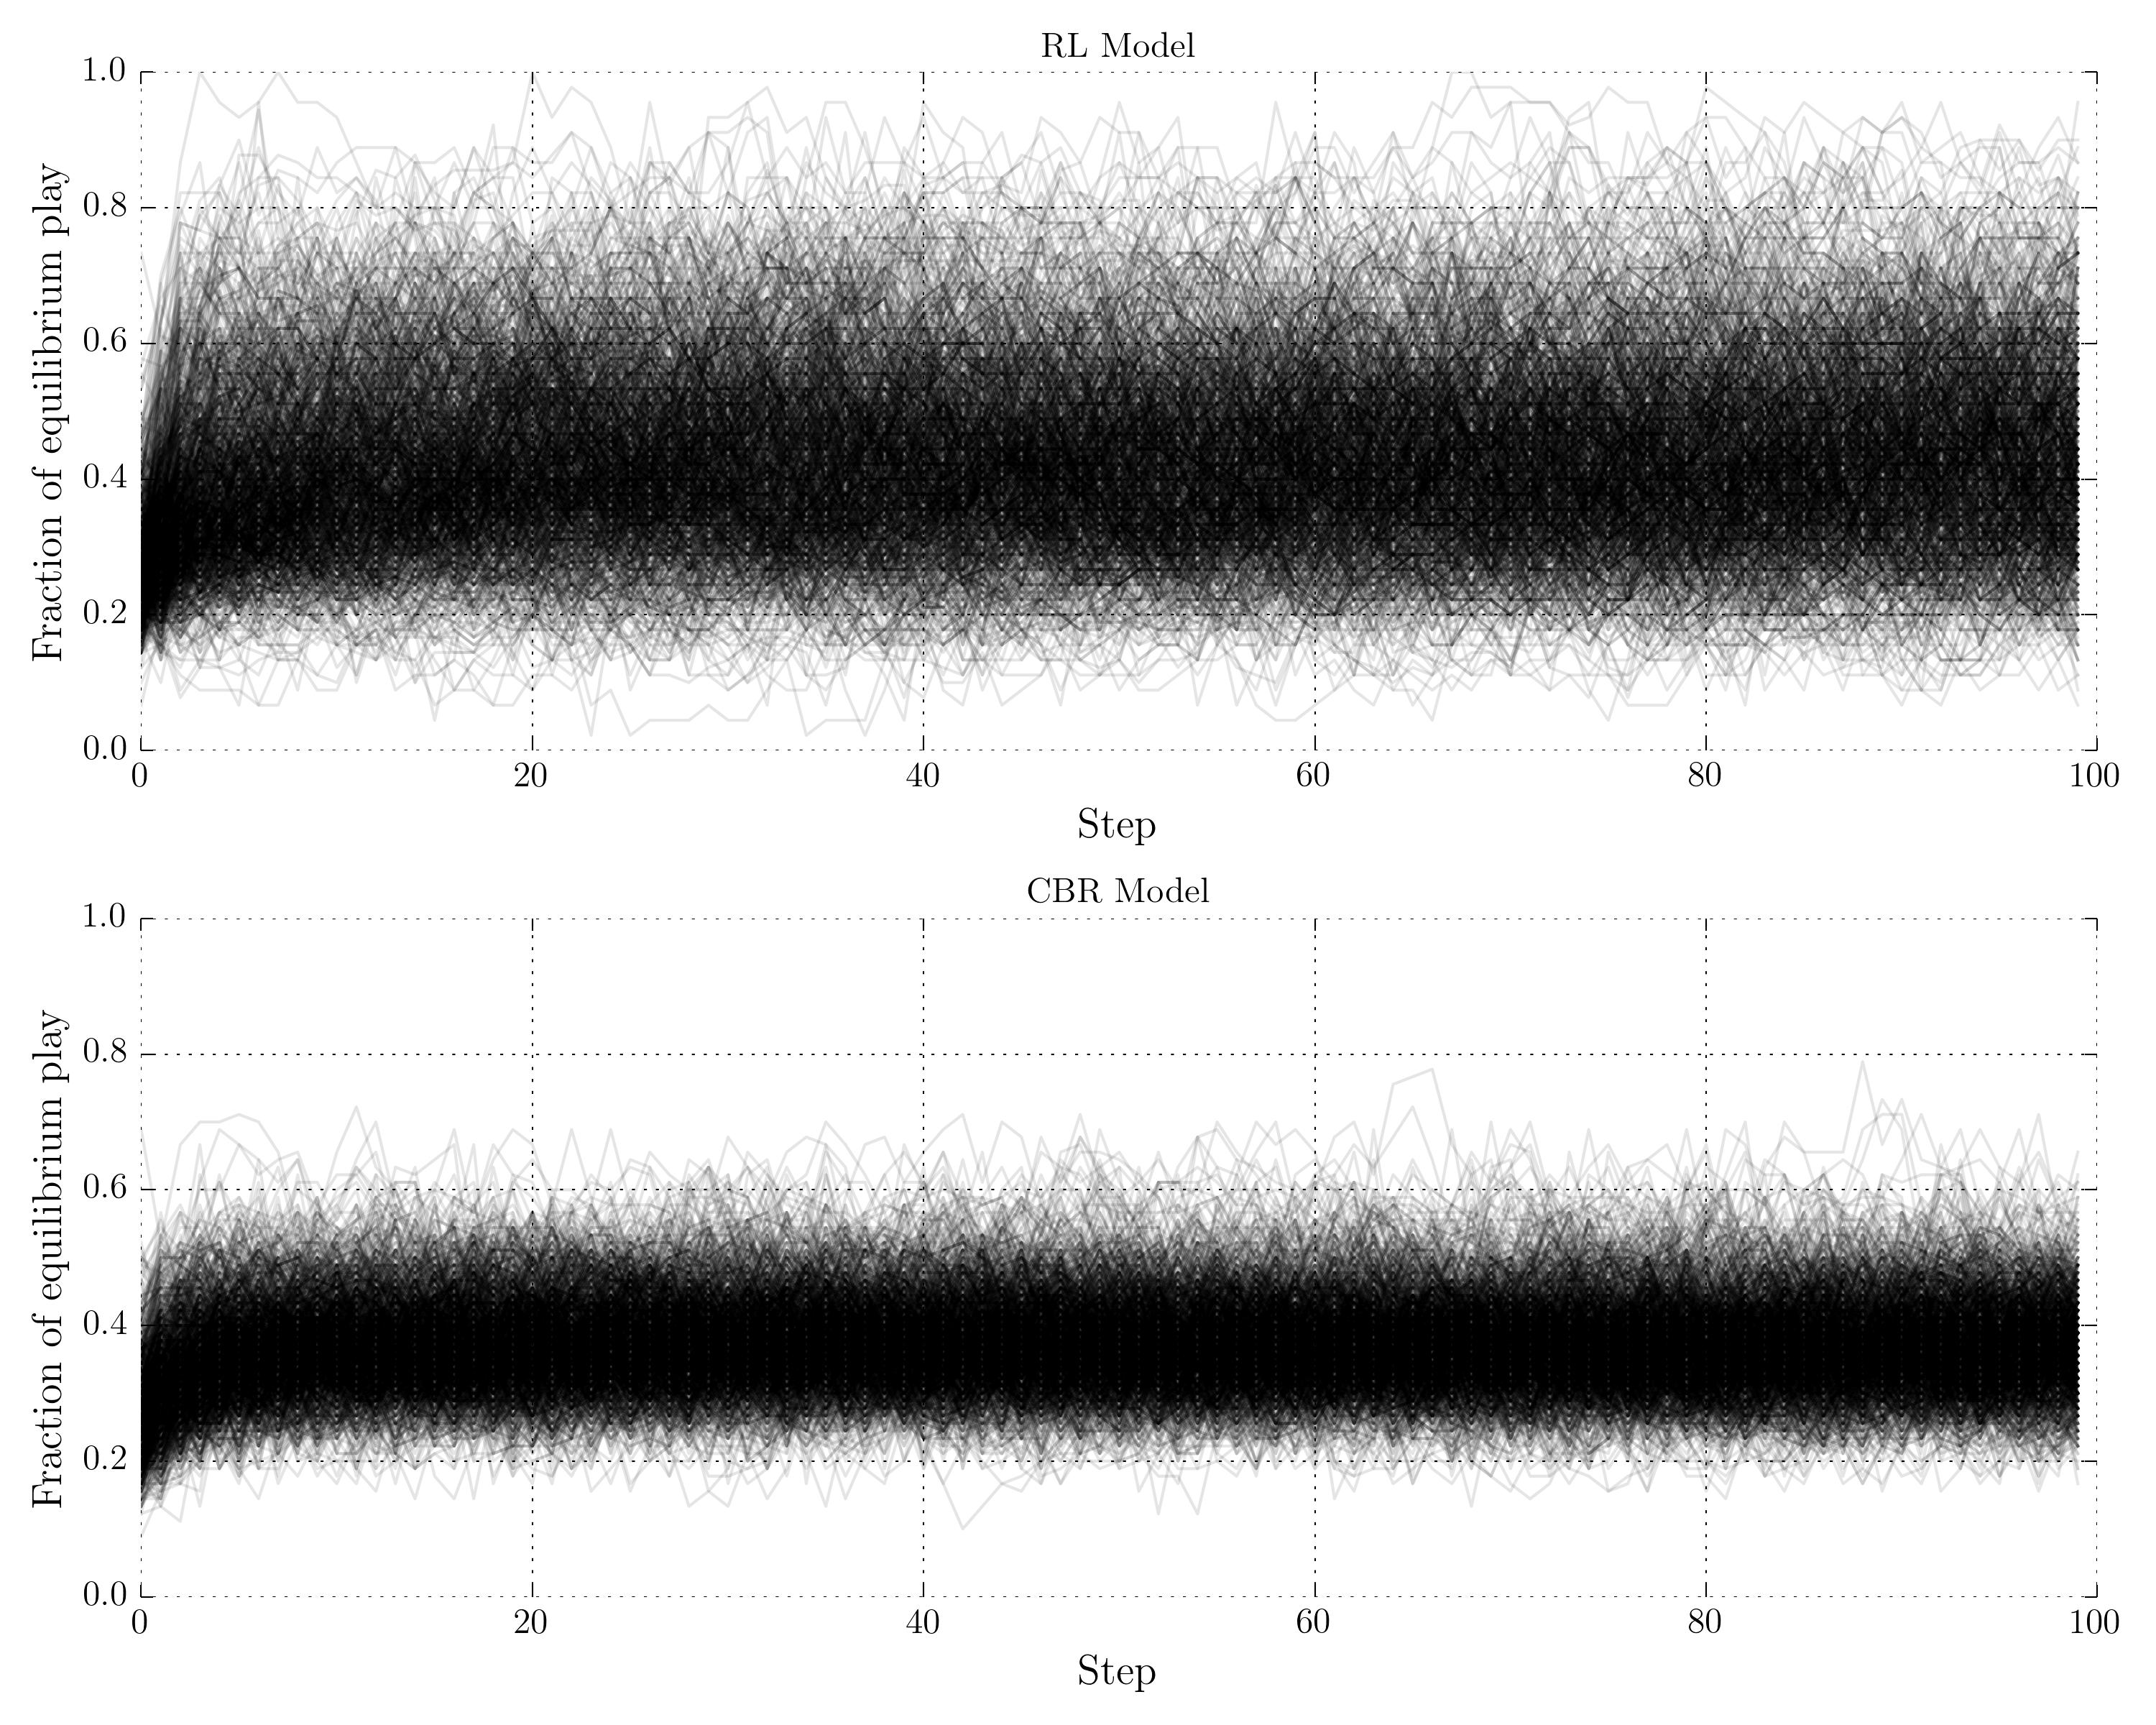
\includegraphics[width=\textwidth]{WarReason/Figures/SC_2_traces}
    \caption{Small Crisis (Dynamic) -- Traces}
    \label{fig:sc2_traces}
    \figSpace
\end{figure}

\begin{figure}[h!]
	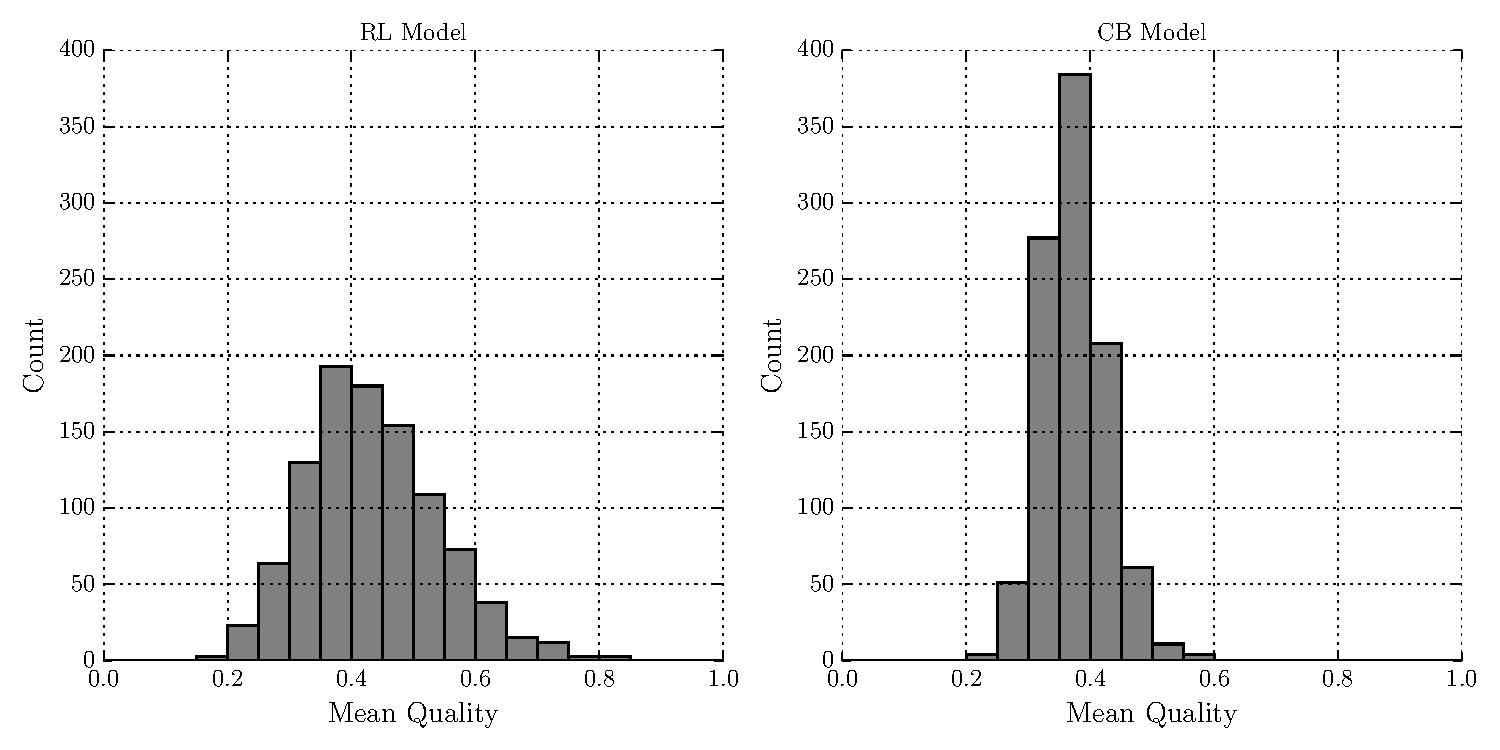
\includegraphics[width=\textwidth]{WarReason/Figures/SC_2_histograms}
    \caption{Small Crisis (Dynamic) -- Quality Distribution}
    \label{fig:sc2_outcomes}
    \figSpace
\end{figure}

\begin{figure}[h!]
	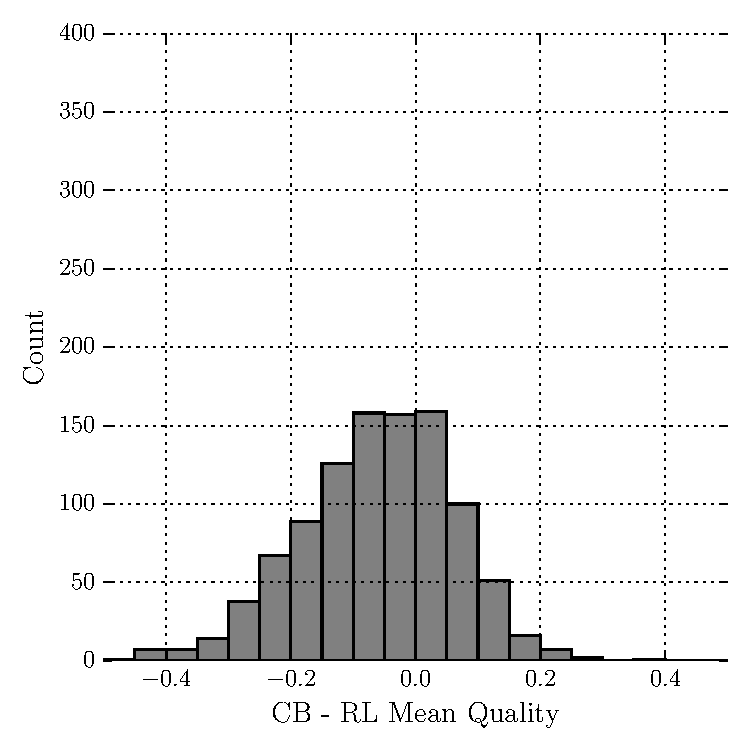
\includegraphics[width=0.5\textwidth]{WarReason/Figures/SC_2_deltas}
    \caption{Small Crisis (Dynamic) -- CB and RL Differences}
    \label{fig:sc2_deltas}
    \figSpace
\end{figure}

\subsubsection{Dynamic Variant}

Next, I repeat the above experiment and analyses with the dynamic model variant, where agent properties change from step to step. Figures \ref{fig:sc2_traces} and \ref{fig:sc2_outcomes} show the traces and distribution of outcomes, respectively. We can immediately see that overall the agents are less likely to play the equilibrium outcome compared to the Static variant, across both decisionmaking models. This is exactly in line with our intuitive expectation -- since each dyad of agents do not have a fixed set of moves to reach equilibrium, and indeed the mix of equilibrium moves across the entire population is changing, the lessons of previous interactions will be less applicable to future ones, making moves based on the learned weights less likely to result in equilibrium. Examination of the outcomes across different learning rates, as shown in Figure \ref{fig:sc2_boxwhiskers} suggests that they do not yield significant differences. This, in turn, suggests that the speed at which agents adjust their behaviors does not substantially affect the behavior the model converges to.
% Build those expectations earlier so we know what 'in line with' them means.
\begin{figure}[h!]
	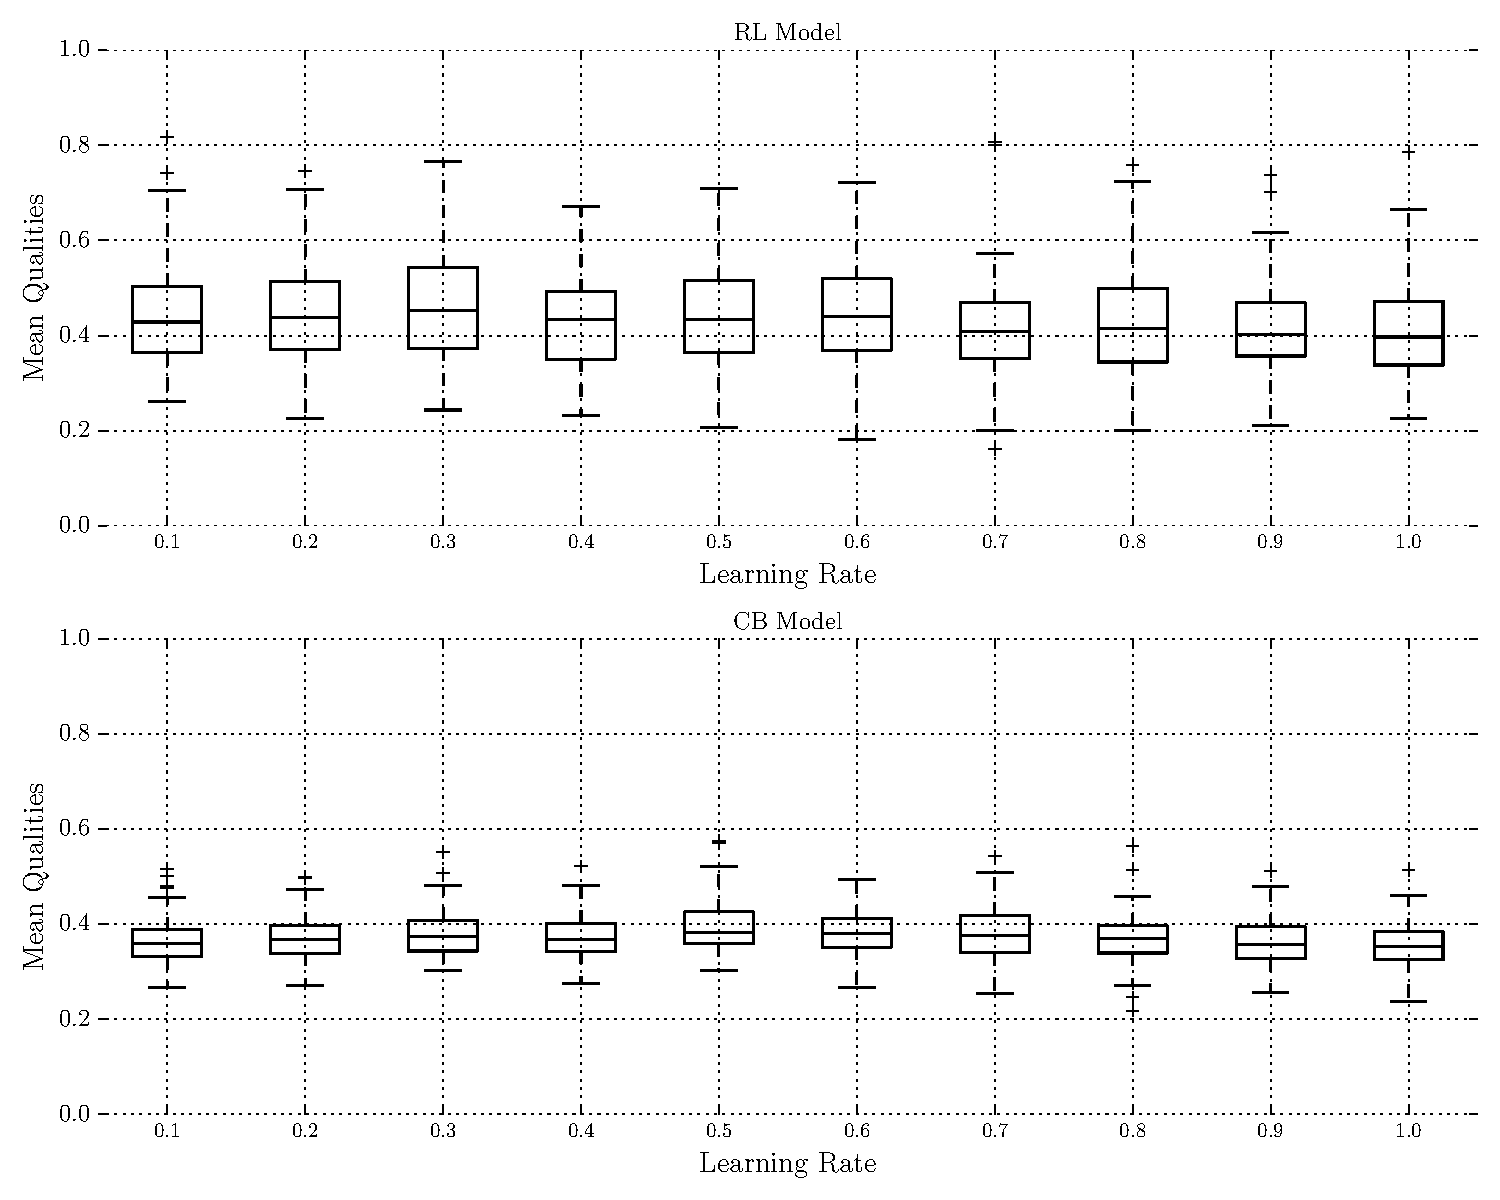
\includegraphics[width=\textwidth]{WarReason/Figures/SC_2_boxwhiskers}
    \caption{Small Crisis (Dynamic) -- Quality by Learning Rate}
    \label{fig:sc2_boxwhiskers}
    \figSpace
\end{figure}

\begin{table}[h!]

	\caption{Small Crisis (Dynamic) -- Logistic Regressions}
	\label{table:sc2_logits}

	\begin{subtable}{\textwidth}
	\begin{center}
		\caption{RL Model}
		%\label{table:sc1_logits}
	\begin{tabular}{lccccc}
		\hline
		            & StatusQuo & Capitulate1 & Capitulate2 &   War1   &   War2     \\
		\hline
		Capitulate1 & -0.13***  & 2.13***     & 0.47***     & -0.51*** & 1.30***   \\
		            & (0.01)    & (0.02)      & (0.01)      & (0.01)   & (0.02)    \\
		Capitulate2 & -0.58***  & 1.39***     & 1.47***     & 0.02***  & -0.35***  \\
		            & (0.00)    & (0.02)      & (0.01)      & (0.01)   & (0.03)    \\
		War1        & -0.24***  & -2.17***    & -0.21***    & 0.42***  & -2.46***  \\
		            & (0.00)    & (0.08)      & (0.01)      & (0.01)   & (0.07)    \\
		War2        & 0.51***   & 0.72***     & -0.65***    & -0.95*** & 1.32***   \\
		            & (0.01)    & (0.03)      & (0.01)      & (0.01)   & (0.02)    \\
		Const.      & 2.49***   & -6.33***    & -4.18***    & -2.82*** & -5.64***  \\
		            & (0.00)    & (0.02)      & (0.01)      & (0.00)   & (0.01)    \\
		\hline
		\hline
		\multicolumn{6}{l}{Standard errors in parentheses.} \\
		\multicolumn{6}{l}{* $p<.1$, ** $p<.05$, *** $p<.01$} \\
		\end{tabular}
		\end{center}
		\tableSpace
	\end{subtable}

	\begin{subtable}{\textwidth}
		\begin{center}
			\caption{CB Model}
			%\label{table:sc1_logits}
		\begin{tabular}{lccccc}
					&			&			  &				&		   &           \\
		\hline
		            & StatusQuo & Capitulate1 & Capitulate2 &   War1   &   War2     \\
		\hline
		Capitulate1 & -0.17***  & 1.26***     & -0.57***    & -0.29*** & 0.87***   \\
		            & (0.00)    & (0.01)      & (0.01)      & (0.00)   & (0.01)    \\
		Capitulate2 & -0.37***  & 0.15***     & 1.22***     & -0.33*** & -0.17***  \\
		            & (0.00)    & (0.01)      & (0.00)      & (0.00)   & (0.01)    \\
		War1        & -0.88***  & -1.20***    & 0.92***     & 0.62***  & -0.69***  \\
		            & (0.00)    & (0.01)      & (0.00)      & (0.00)   & (0.01)    \\
		War2        & -0.49***  & 1.05***     & -1.21***    & 0.17***  & 1.16***   \\
		            & (0.00)    & (0.01)      & (0.01)      & (0.00)   & (0.00)    \\
		Const.      & 0.05***   & -3.28***    & -2.32***    & -0.77*** & -3.09***  \\
		            & (0.00)    & (0.00)      & (0.00)      & (0.00)   & (0.00)    \\
		\hline
		\hline
		\multicolumn{6}{l}{Standard errors in parentheses.} \\
		\multicolumn{6}{l}{* $p<.1$, ** $p<.05$, *** $p<.01$} \\
		\end{tabular}
		\end{center}
	\end{subtable}
	\tableSpace
\end{table}

\begin{figure}[h!]
	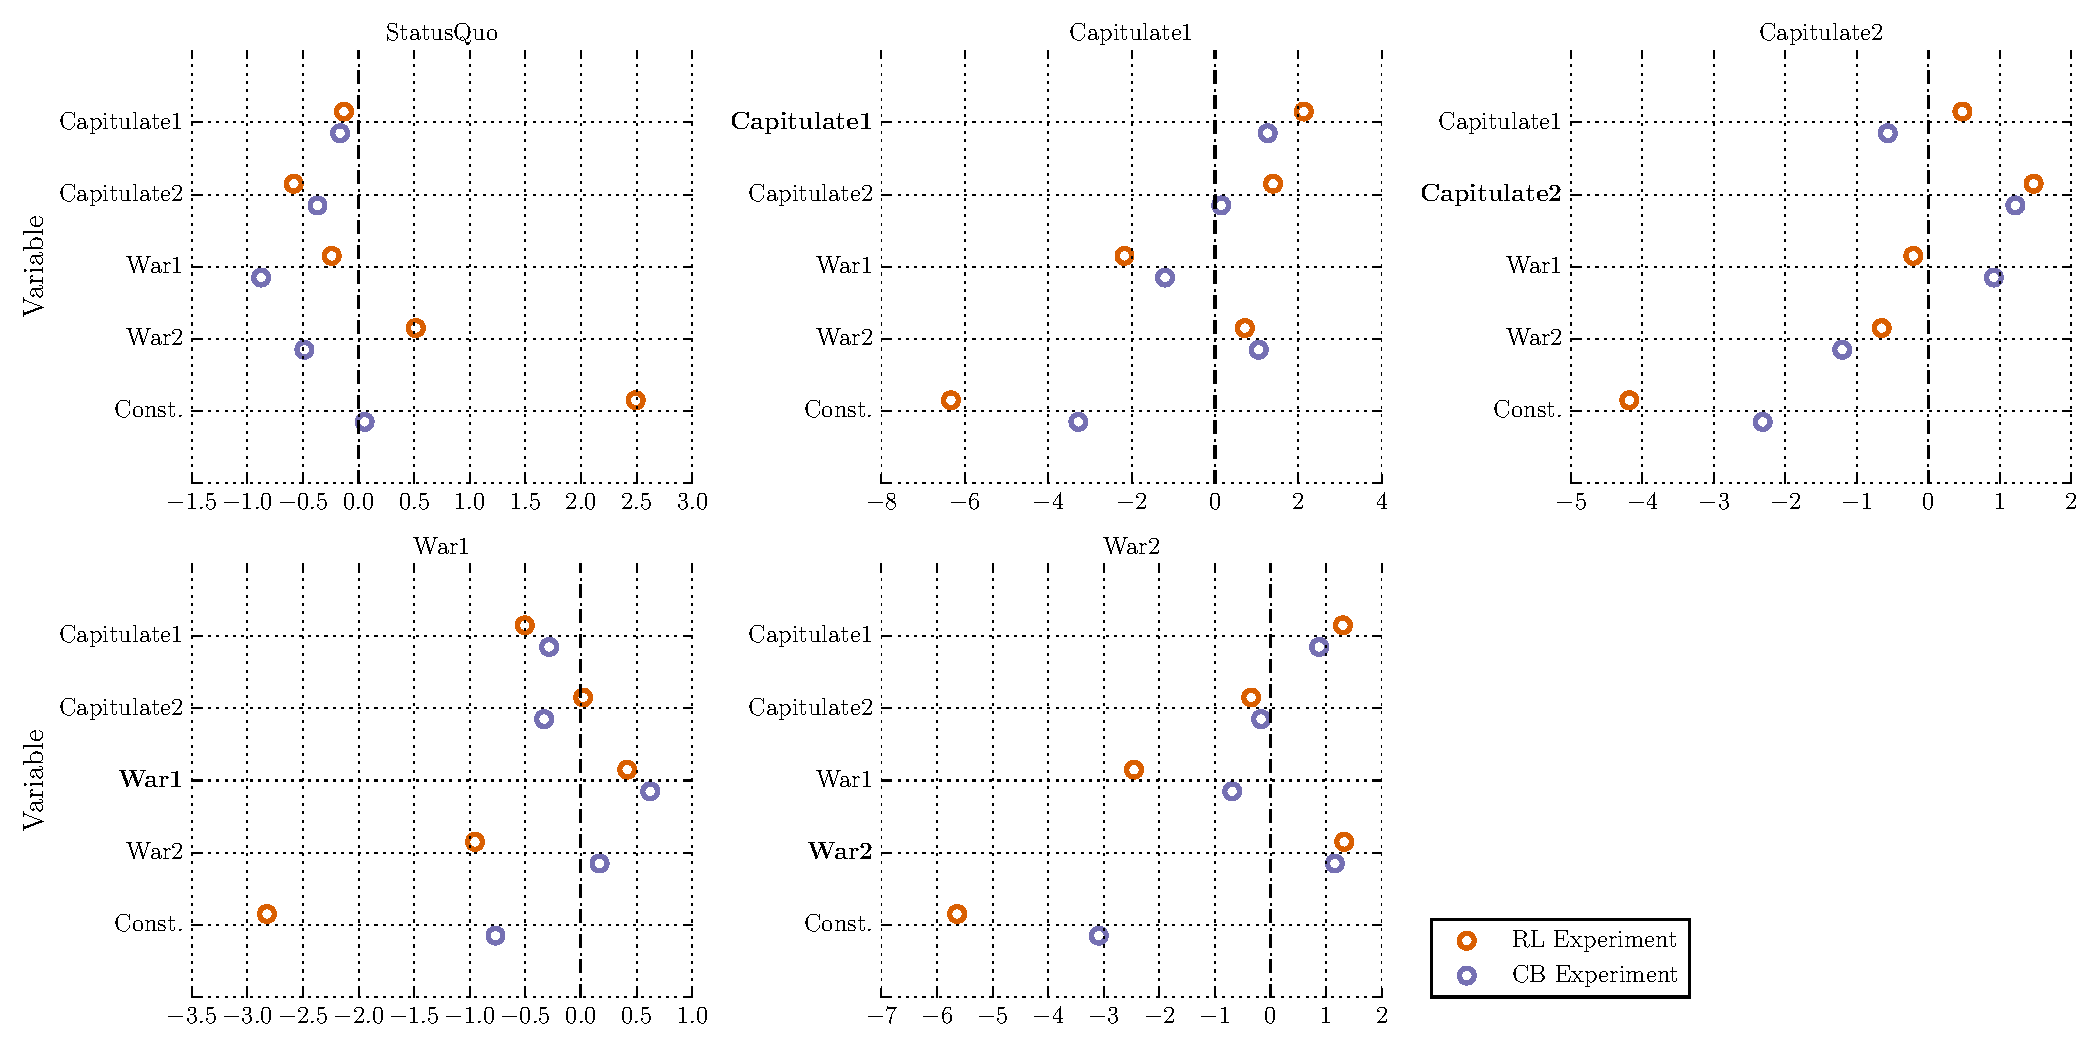
\includegraphics[width=0.95\textwidth]{WarReason/Figures/SC2_Coeffs}
    \caption{Small Crisis (Dynamic) -- Logistic Regression Coefficient Plots}
    \label{fig:sc2_coeffs}
    \figSpace
\end{figure}

A more surprising result is that the CB decisionmaking model does not outperform the RL model.  Figure \ref{fig:sc2_deltas} shows the distribution of differences between the model qualities; it has a mean of -0.06, indicating that on average the CB agents perform very slightly worse than the RL agents. This is confirmed by the logistic regressions, reported in Table \ref{table:sc2_logits} and shown visually in Figure \ref{fig:sc2_coeffs}. As with the regressions done on the Static variant results, the equilibria are still positive predictors of a corresponding outcome. Unlike with the Static variant, however, the equilibrium is not a stronger predictor of the outcome of the CB models than of the RL models. This contradicts the hypothesis that the CB decisionmaking model is broadly superior to the the RL decisionmaking model in terms of approaching rational play.

In the previous model variant, the CB agents were implicitly learning best moves against each particular agent. In this variant, since agent properties are changing, there is no single best response to be learned. Additionally, with ever-changing agent properties, there are more potential coordinates populating the case history space more densely. The equilibrium moves exhibit discontinuities across this space; however, the updating rule, whereby a new interaction updates both its own coordinate point and those of the nearest previous case, mean that moves appropriate for one equilibrium but not the other may propagate across these discontinuities -- essentially, agents consider two cases more similar than they actually are. 

\subsection{International Interaction Game} \label{iig_results}

The previous, simple model allowed me to verify that the decision models were implemented properly, with the code corresponding to the model description. More substantively, the results reported above suggest that multiple agents are capable of learning to play extensive-form games against each other in a manner approaching rational behavior, in line with my initial hypothesis. Furthermore, the difference in performance of the RL and CB models between the static and dynamic variant complicates expectations for the real world, which is itself dynamic. With these results in mind, I move from the notional, simplified international system to the full International Interaction Game (IIG) with the EUGene data, as described in Section \ref{sec:iig_description}. 

I carry out these experiments as follows. For each of the RL and CB decisionmaking models, I instantiate 105 model runs\footnote{The non-round number is due to model runs being executed in parallel on 15 cores on 16-core servers.}, with all agents utilizing the same decisionmaking model with fixed learning rates: 0.1 for the RL model, and 0.2 for the CB model. Each instantiation includes one agent for each unique country in the EUGene dataset, and is run as described in Section \ref{sec:iig_description}. I record the outcome for each interaction from each instantiation, and compare them to the equilibrium outcomes and observed events. There are thirteen possible outcomes of the extensive-form game tree, meaning that if agents were to play at random there would be a 7.7\% chance of observing an outcome equal to the equilibrium. Figure \ref{fig:ex2_traces} shows the fraction of interactions by year ending in the IIG equilibrium outcome. There are several things immediately obvious: as with the simplified model, we never see convergence to perfect equilibrium behavior. Unlike with the simplified model, however, there is not an obvious rapid initial burn-in period followed by relative stability. Instead, there is a broad range of traces showing different rates of improvement, with occasional sharp dips and upward spikes. 

\begin{figure}[h!]
    \centering

    \begin{subfigure}[t]{\textwidth}
        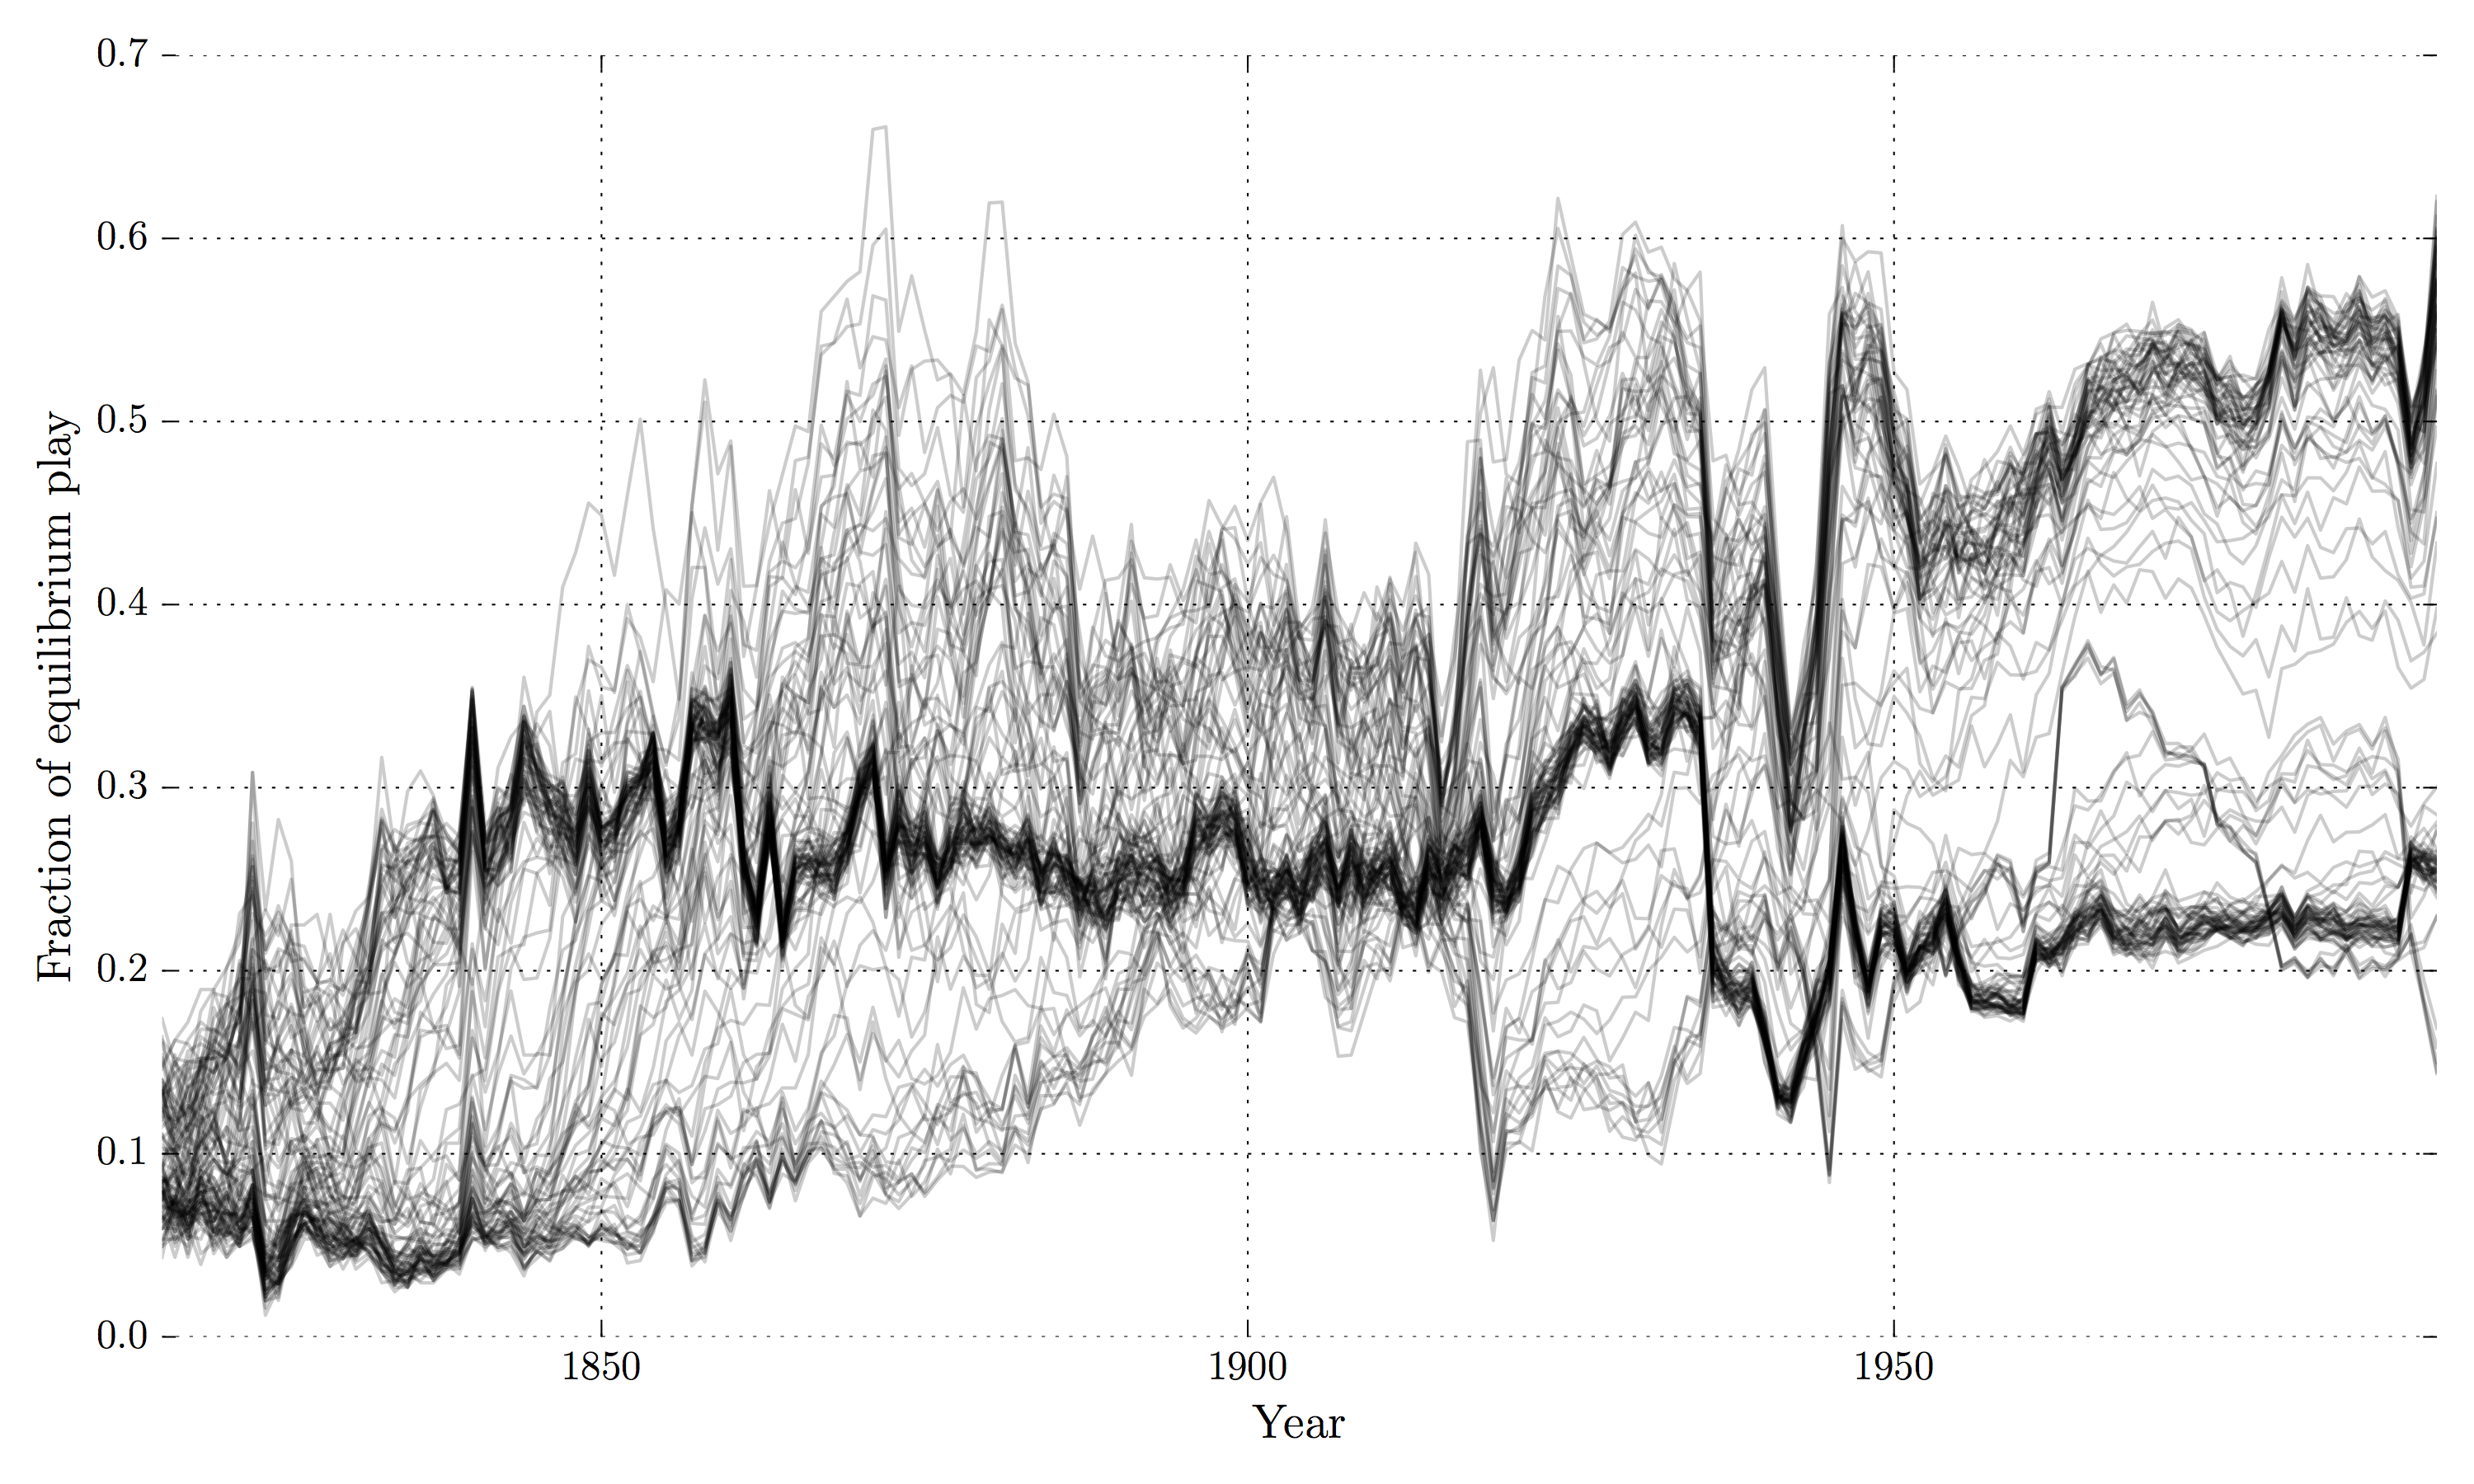
\includegraphics[width=\textwidth]{WarReason/Figures/RL_equilibria}
        \caption{Reinforcement Learning Model}
    \end{subfigure}
    
    \begin{subfigure}[t]{\textwidth}
        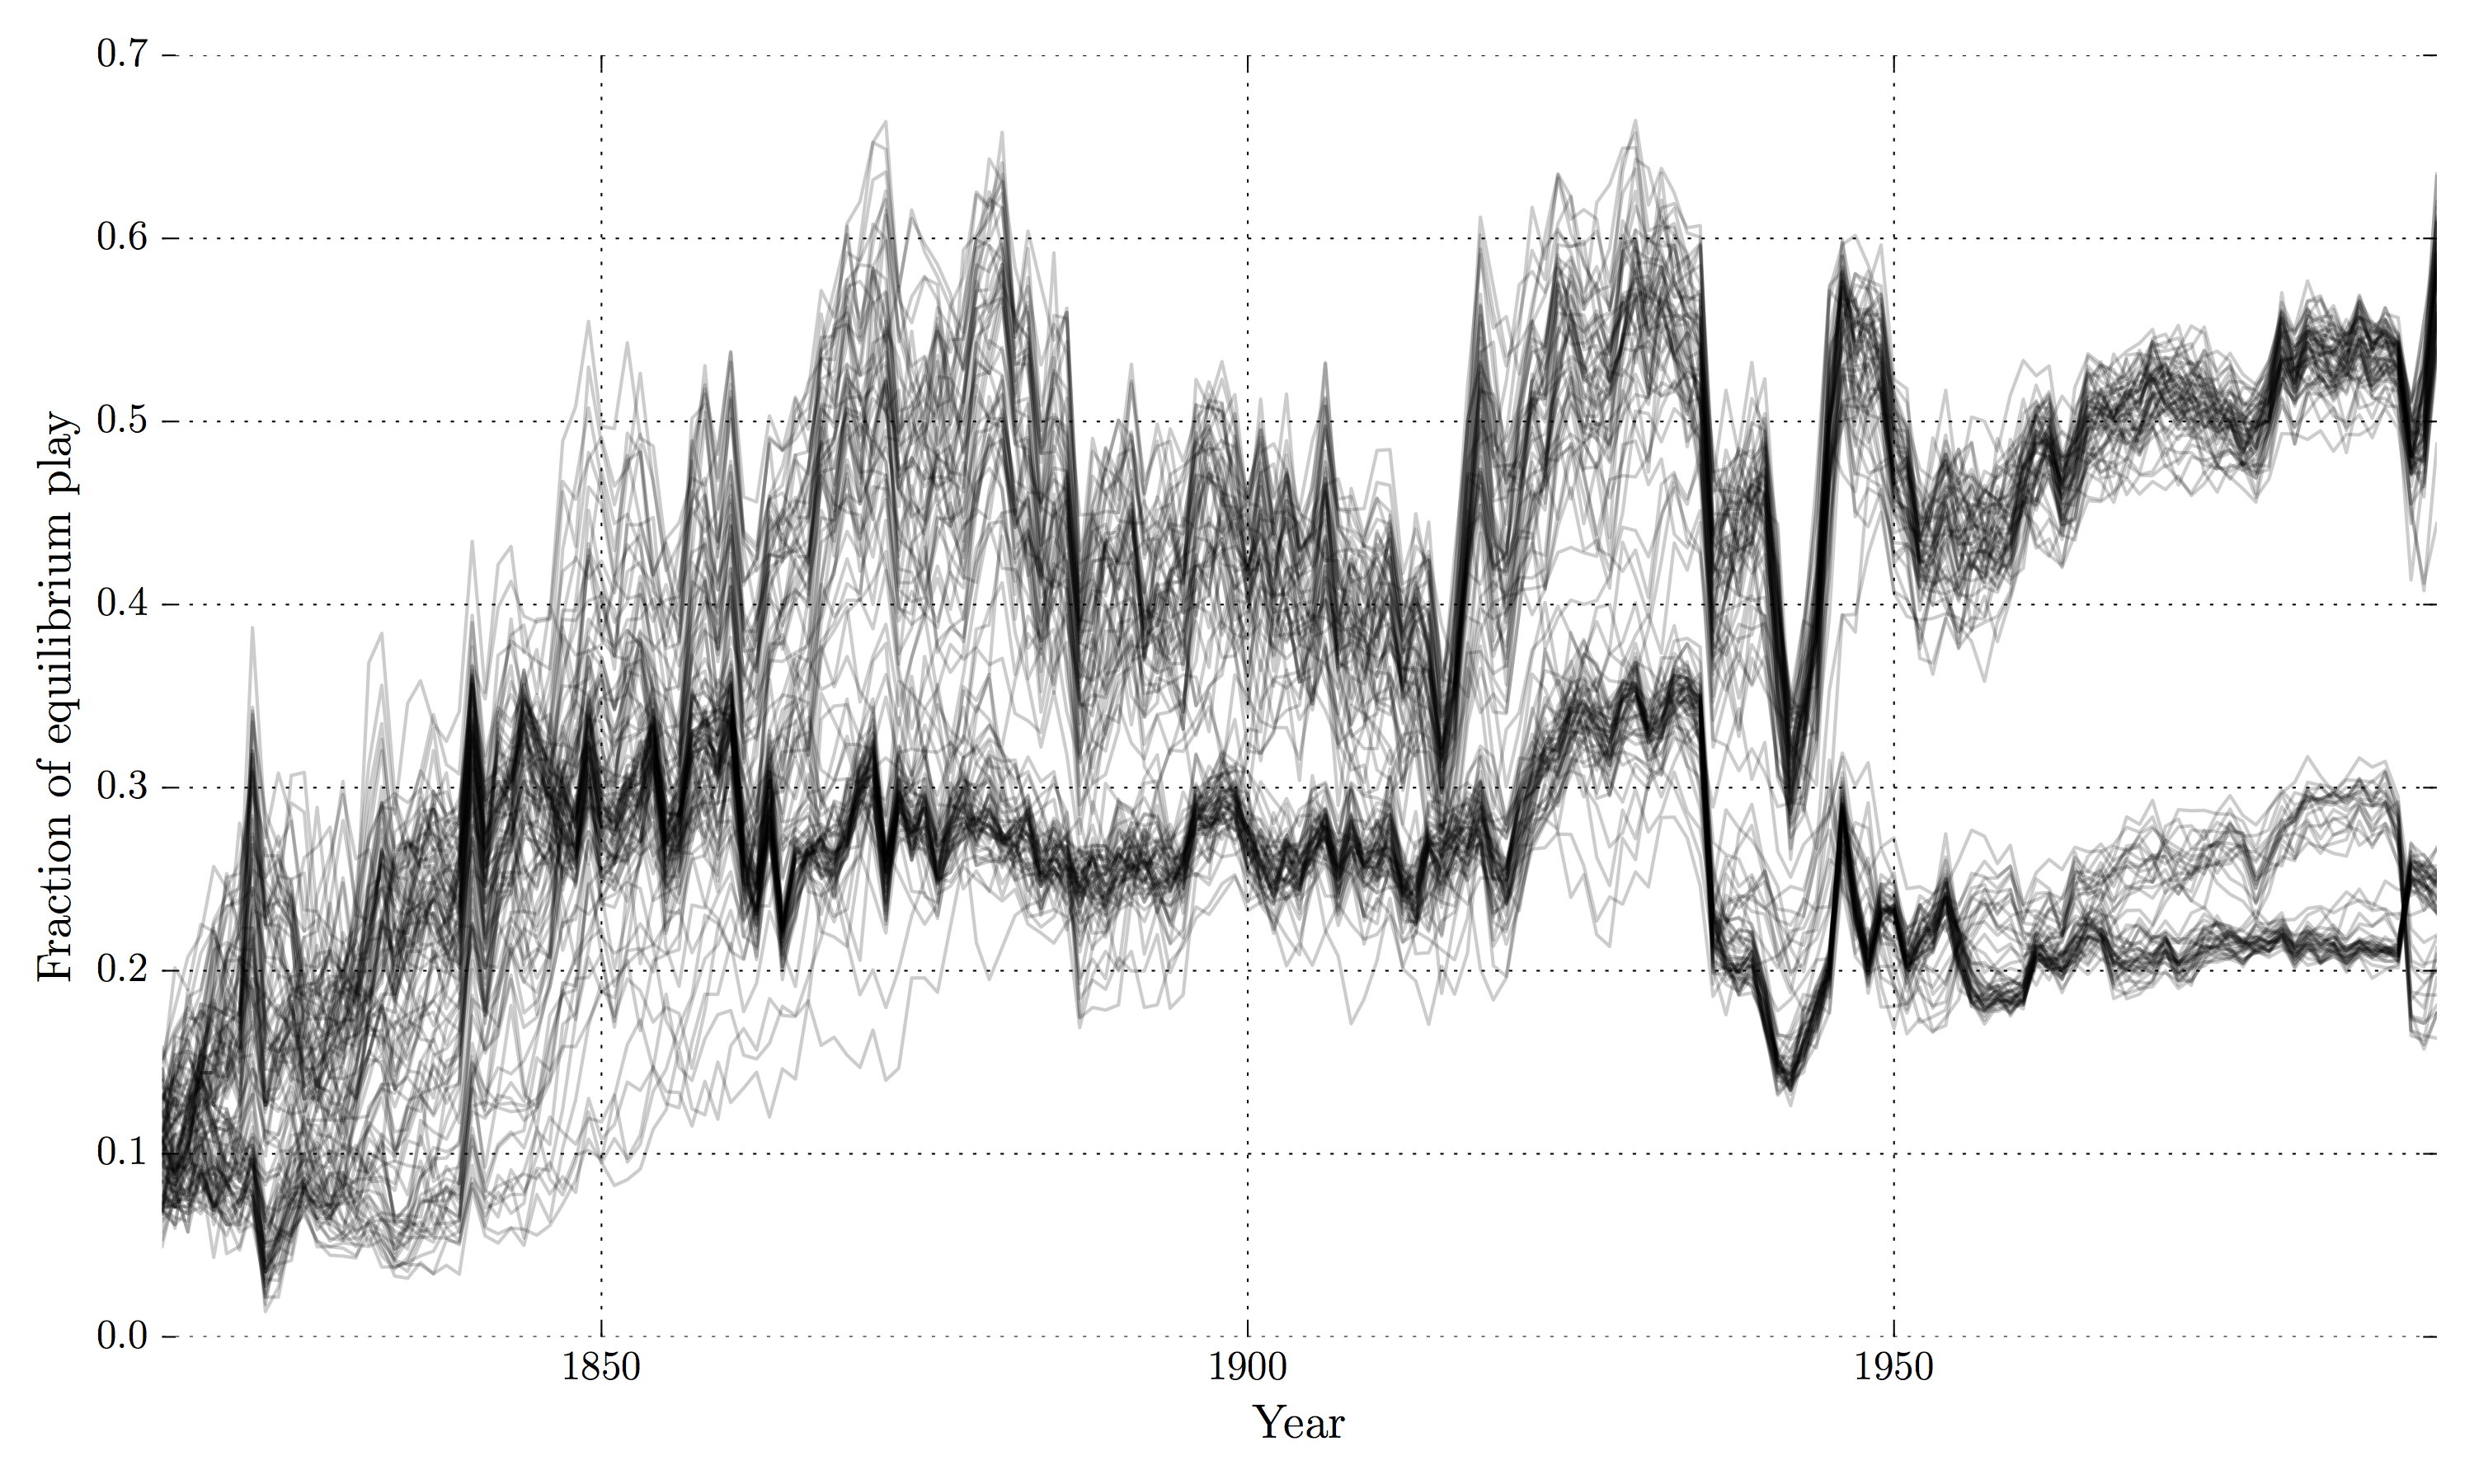
\includegraphics[width=\textwidth]{WarReason/Figures/CB_equilibria}
        \caption{Case-Based Learning Model}
    \end{subfigure}

    \caption{Fraction of Interactions with Equilibrium Outcome}
    \label{fig:ex2_traces}
    \figSpace
\end{figure}

It appears that the rate of improvement across the majority of CB runs is initially greater than for the RL runs; in particular, all CB runs rise above the fraction of equilibrium outcomes expected by chance earlier than the RL runs. However, there is not a clear stable performance rate reached for either decisionmaking model, with multiple substantial shifts in the rate of equilibrium play. In fact, across all the different runs, these shifts occur at similar points, in some cases in different directions. Note in particular the very obvious effects of the two world wars. Those conflicts themselves are outside the scope of the IIG and its variants: they were heavily multilateral, took place across multiple years, and radically changed the states present in the international system and alliance network between them. It appears to be the case that the shocks of the world wars substantially changes the distribution of equilibrium moves for the different agents. In some runs, this leads to a significant drop in equilibrium performance, while in others the agents either successfully rapidly adapt or have previously learned distributions of behaviors which prove to be improvements in the new environment. In contrast, following World War II, there is no similar improvement, with the majority of traces demonstrating rapid deterioration in equilibrium play. 

Across both the pure reinforcement learning and case-based learning decisionmaking model variants, there appear to be several overall attractors, with multiple model instantiations demonstrating similar behavior. These attractors are visible in Figure \ref{fig:ex2_traces} as the darker regions where multiple line traces come together. Both variants have one attractor with a fraction of equilibrium play at approximately 0.25, which emerges early on. Across both variants, this attractor shows a sharp falloff approximately during the 1930s, then rebounds somewhat, and stabilizes from 1950 until the end of the model timeframe. Both variants also exhibit a second attractor which emerges later, at a substantially higher equilibrium fraction. In the RL variant, the second attractor emerges most during the mid-1930s; in the CB variant, it emerges earlier, beginning from the mid-1860s onward, though the attractors' traces converge to a tighter band after 1950 here as well. Note, however, that even the lower attractors show substantially better mean performance than if the agents were choosing moves at random.

These results indicate that the agents are learning to play the equilibrium strategies with one another over time, albeit very imperfectly. The next question, then, is whether this behavior resembles the observed behavior of real actors. Figure \ref{fig:eq_correct} shows the annual fraction of dyads by year where the observed event, as recorded by the COW Militarized Interstate Dispute data \citep{palmer_2015}, matches the IIG equilibrium outcome. As we can see, the equilibria outcomes are rarely observed directly -- the overall mean across all dyads is 12\%, or only slightly better than random. It is important to keep in mind that the vast majority of these dyads exhibit Status Quo outcomes and are not politically relevant, involving distant states with few if any directly overlapping interests or ability or desire to start a conflict with each other. Similarly, the majority of model runs yield very small fractions of correctly-predicted outcomes: only a mean of 2\% for the RL decisionmaking model (worse than random), and 7\% (approximately the same as by chance) for the Case-Based decisionmaking model, across all model runs for each. Figure \ref{fig:ex2_correct} shows the fractions of annual dyads where the outcome matches the observed event for all model runs. While the majority of model instantiations generate extremely low rates of correct outcomes, there are some where the rate of correctly-predicted outcomes is substantially higher by the end of the run. Only 18 of the RL instantiation runs (17\%) generate the observed outcomes at a higher rate than random by the final year of the data, and 3 do so in over half of all interactions. Better, 26 of Case-Based runs (25\%) generate better-than-random predictions, while 15 (14\%) generate the observed outcome over half the time. The traces in these cases indicate that the rate of observed outcomes is high across the majority of the run history, and tends to increase over time. This suggests that the higher accuracy is a robust phenomenon within these instantiations, rather than a statistical fluke within a single year. While the fraction of runs generating these predictions are a minority, they are not insubstantial. These results indicate that the observed outcomes, in the aggregate, can be derived from one of the sets of behaviors the agents converge to across several sets of decisionmaking models and instantiations. This, in turn, suggests that the observed outcomes are satisficing: they yield utilities which encourage all the agents to continue, with increasing frequency, to play the moves which will lead to those outcomes.

\begin{landscape}

	\begin{figure}[h!]
	    \centering
		\begin{subfigure}[t]{\textwidth}
	        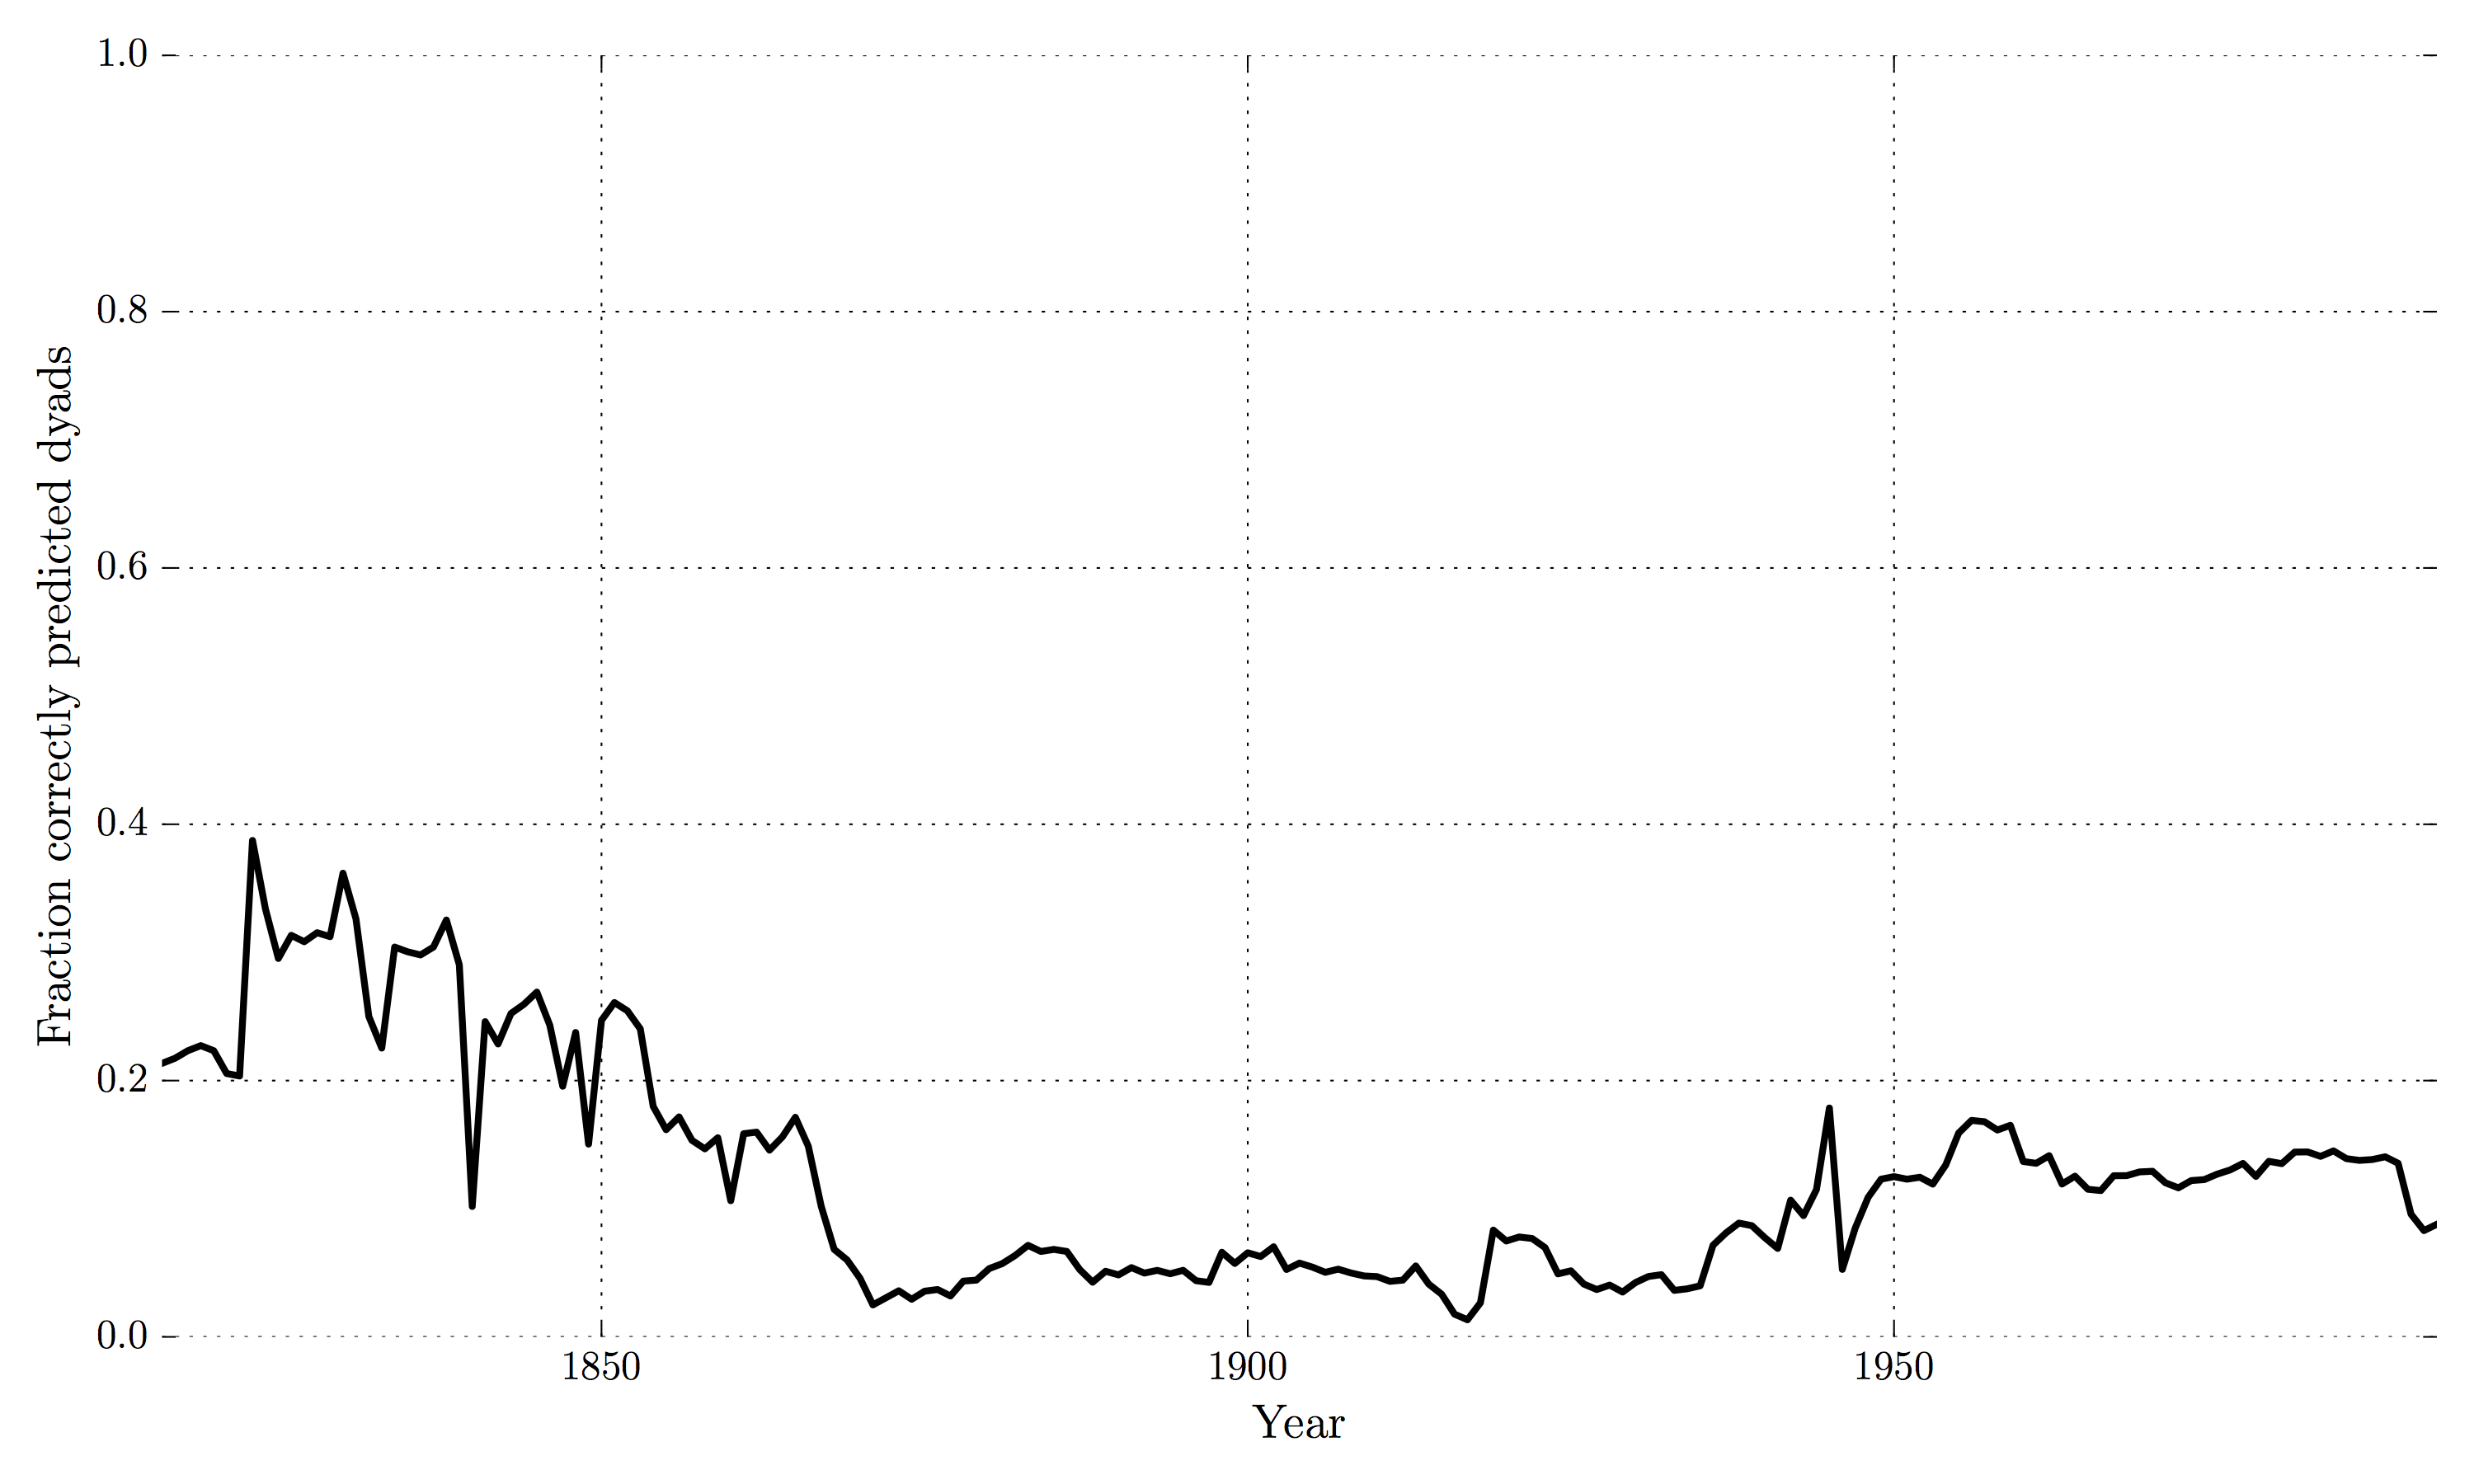
\includegraphics[width=0.7\textwidth]{WarReason/Figures/EQ_correct}
	        \caption{IIG Equilibrium Outcome}
	        \label{fig:eq_correct}
	    \end{subfigure}

	    \begin{subfigure}[t]{0.7\textwidth}
	        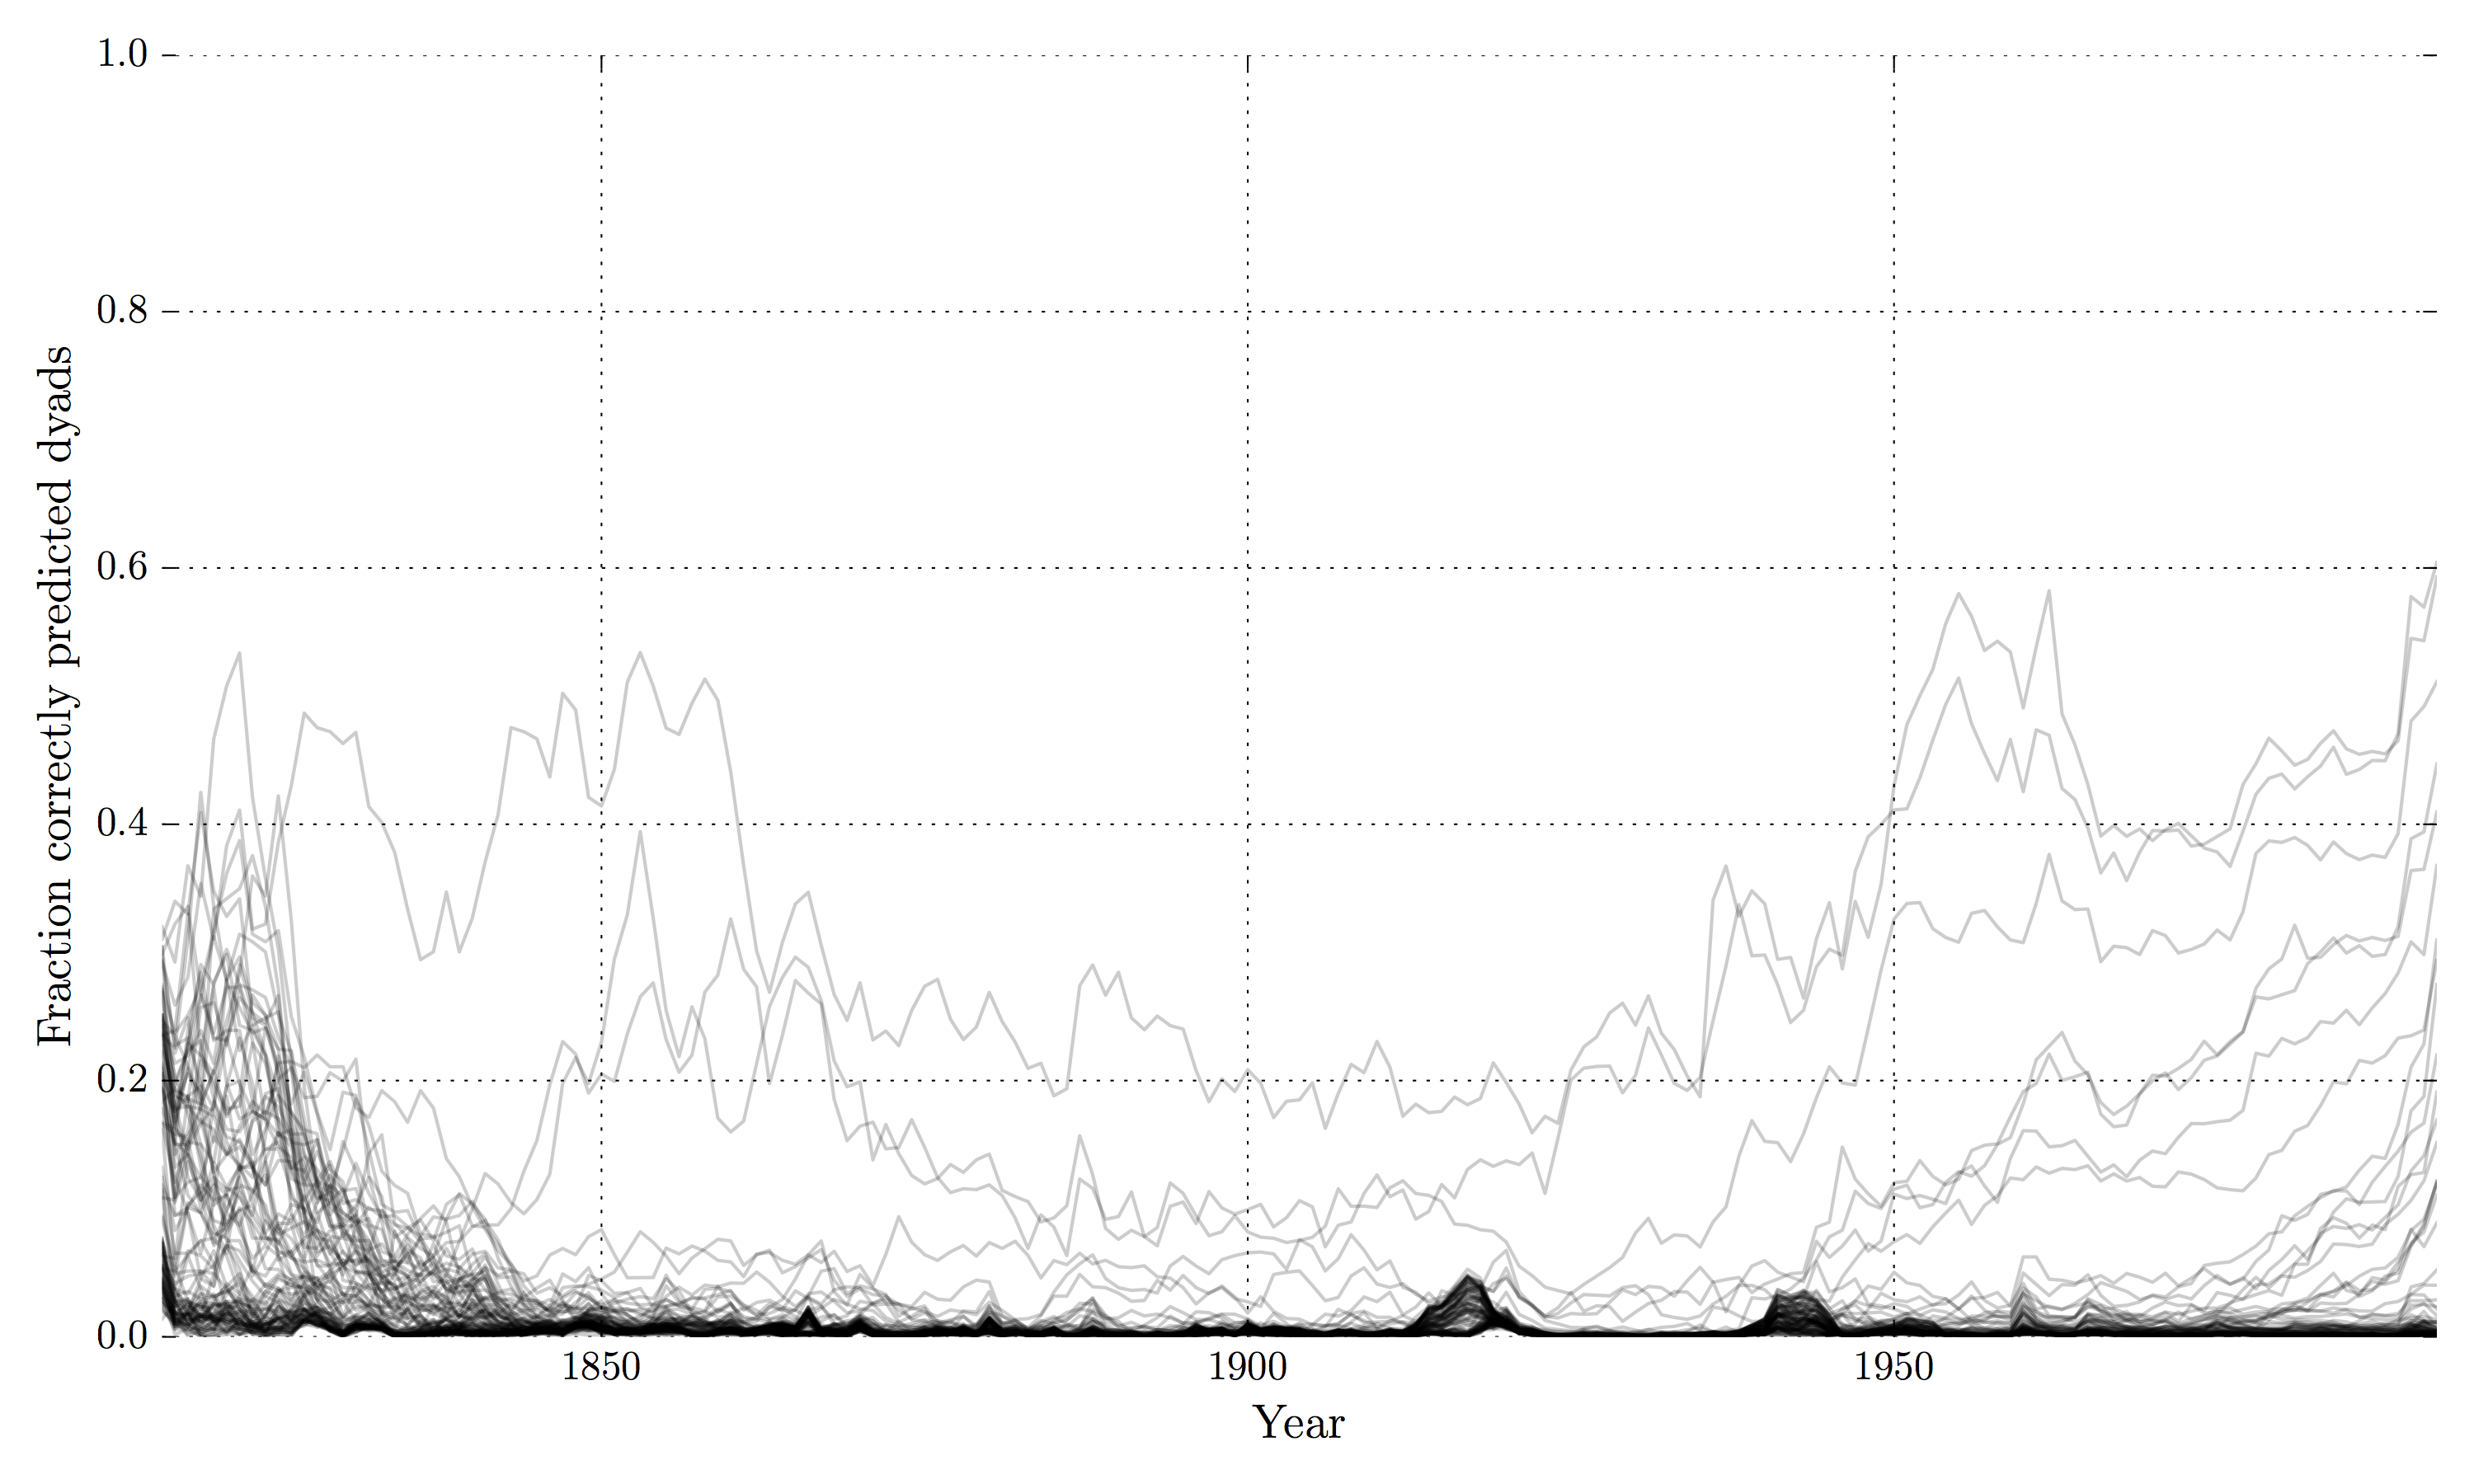
\includegraphics[width=\textwidth]{WarReason/Figures/RL_correct}
	        \caption{Reinforcement Learning Model}
	    \end{subfigure}
	    \begin{subfigure}[t]{0.7\textwidth}
	        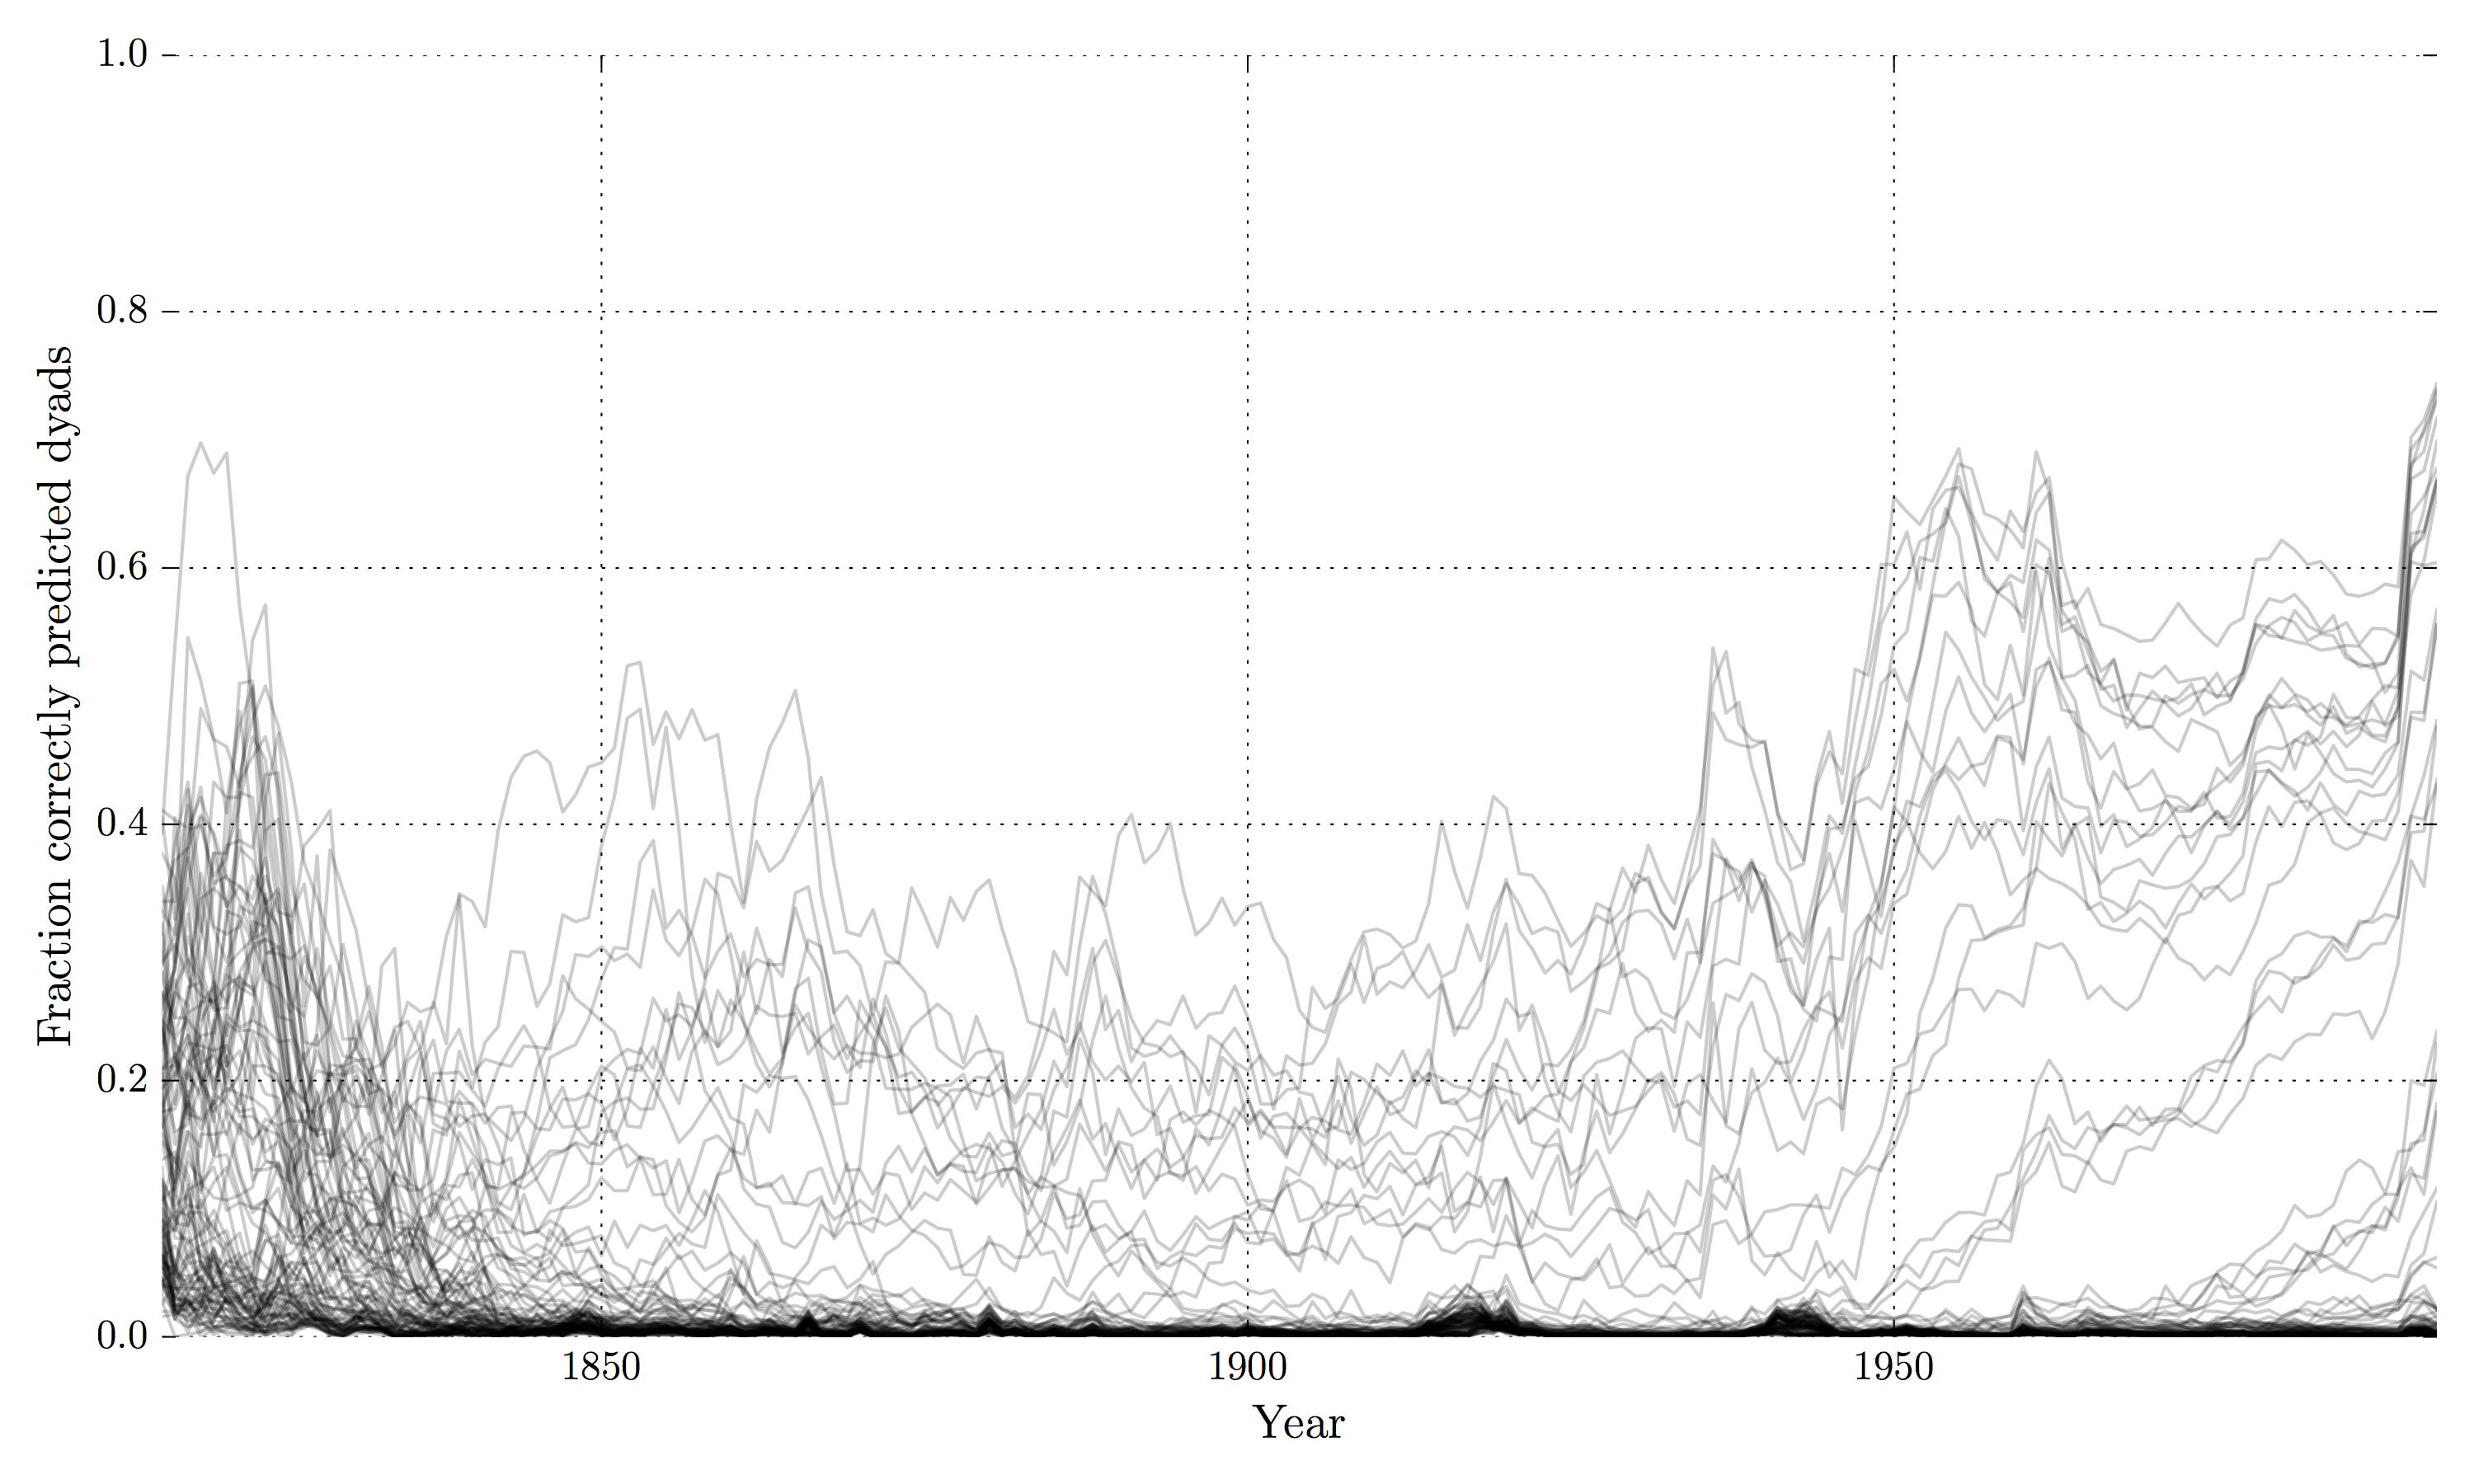
\includegraphics[width=\textwidth]{WarReason/Figures/CB_correct}
	        \caption{Case-Based Learning Model}
	    \end{subfigure}

	    \caption{Fraction of Interactions with Correctly-Predicted Outcome}
	    \label{fig:ex2_correct}
	    \figSpace
	\end{figure}

\end{landscape}

With these results in hand, we can proceed to test whether the model outcomes are a statistically useful predictor of the observed events. As demonstrated in Figure \ref{fig:eq_correct}, the IIG equilibrium is not a direct prediction of observed events; instead, \citet{bdm_1992} and \citet{bennett_2000} use it as a statistical predictor, arguing that estimating a particular equilibrium makes it more likely (though far from certain) that we will observe a corresponding event in the historic data. I apply a similar test to the model outputs. Since the learning models take some number of interactions for their initial learning, it is sensible to drop these early interactions from our analysis as a burn-in period. I could not identify a formal method to determine how long this period ought to be. Based on the traces in Figure \ref{fig:ex2_traces}, the main attractors across the decision models begin to appear at approximately 1850; for this reason, I choose this year as the cutoff for the burn-in period.

I start by replicating the findings of the prior studies. Table \ref{table:eq_regressions} shows the results of logistic regressions with the observed events of each post-1850 dyad as the dependent variables and the IIG equilibria as the independent variables \footnote{Strictly speaking, the correct regression for this case is a multinomial logit, as in \citet{bennett_2000}, since the outcomes of each interaction are mutually exclusive. However, the datasets produced by the 105 instantiations of each model are too large for a multinomial logit to be computationally tractable. In order to keep the model tractable, I treat each outcome as an independent variable. This method provides a worse fit, but allows the coefficients to be interpreted the same way.}. This is a simplified model, without many of the controls (e.g. for polity type, or length of peace) introduced by \citet{bennett_2000}. These regression results are comparable to those reported in \citet{bennett_2000}, providing moderate support for the hypothesis of the IIG equilibrium as an outcome predictor prior to adding in the various controls. More importantly, these results provide a baseline against which we may compare the results of similar regressions using the decisionmaking model interaction results.

%% table:eq_regressions showing logit results via IIG Equilibrium outcomes goes here

%% table:ex1_regressions and table:ex2_regressions GO ABOUT HERE, showing coefficients from RL and CB logits.

Tables \ref{table:rl_regressions} and \ref{table:cb_regressions} show the results of the same logistic regressions on the outcomes of the post-1850 interactions in the RL and CB models, respectively. The coefficients for both models as well as the equilibrium model are shown visually in Figure \ref{fig:coef_plots}, below. We can see that the learning model coefficients are similar to those of the equilibrium models, showing moderate support for the hypothesis that the model outcomes are a predictor of the observed outcome. The level of support varies between outcome types. For Acquiesce events, the coefficients on the corresponding model outcomes are significant and positive, while those on the opposite outcome (the acquiescence of the other party) are negative. However, this is not the case for Capitulate events, where capitulation outcomes in both directions have a positive coefficient. Importantly, War and Negotiation outcomes are both positive predictors of observing corresponding events. However, War outcomes are also predictors of observing Negotiation events -- which suggests that the model is correctly capturing cases where a conflict is likely, but that some of those conflicts are in fact resolved via negotiation rather than war. Similarly, note that the Capitulation outcomes are also positive predictors of War events, and vice versa. These outcomes are adjacent to one another on the game tree, which provides support for the structure of the game tree itself. It suggests that the model agents are playing down to the correct subgame of the game tree, with one agent making a single move different from what was observed.

\begin{figure}[h!]
	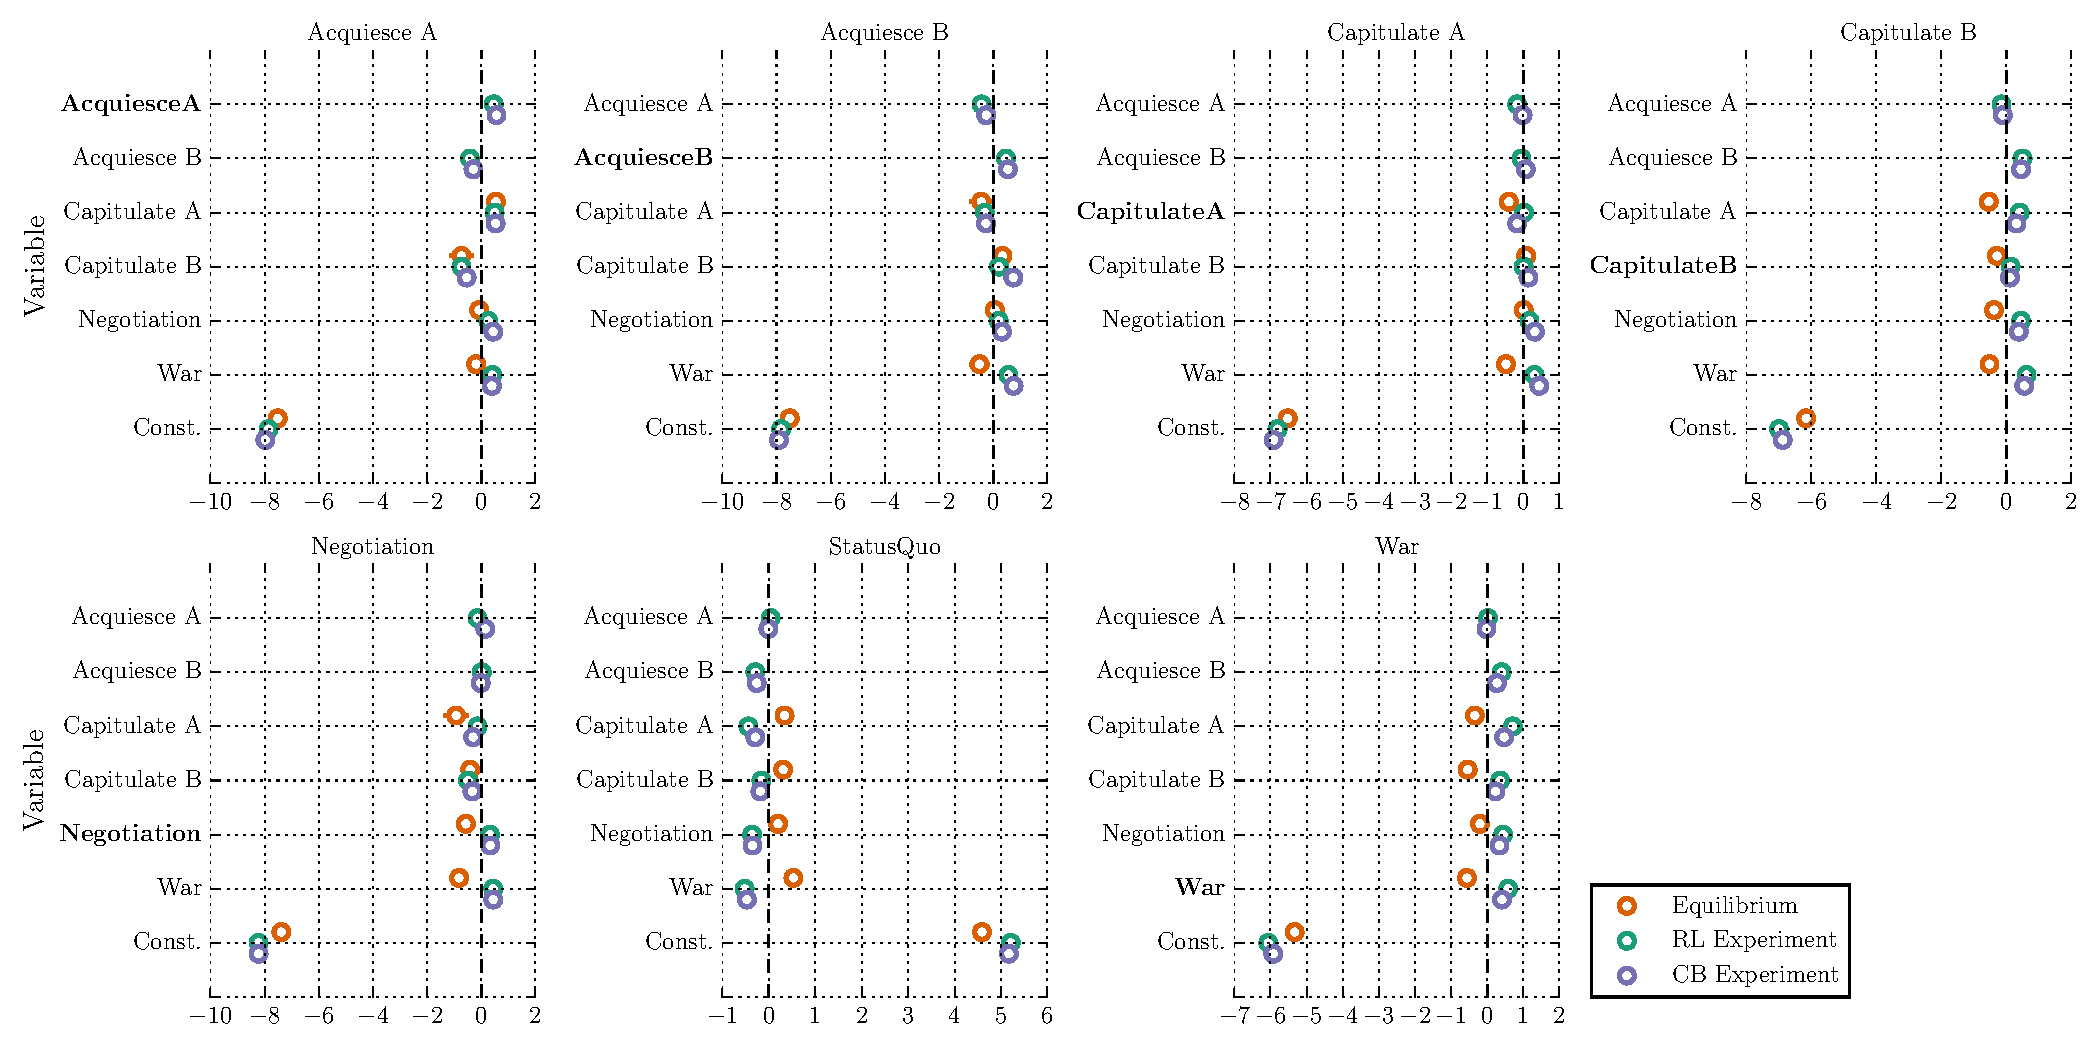
\includegraphics[width=\textwidth]{WarReason/Figures/WarReason_Coeffs.pdf}
    \caption{Logistic Regressions Coefficient Plots}
    \label{fig:coef_plots}
    \figSpace
\end{figure}

\begin{landscape}
\begin{table}
	\begin{center}
		\caption{IIG Model Equilibrium -- Logistic Regressions}
		\label{table:eq_regressions}
	\begin{tabular}{lccccccc}
	\hline
	             & Capitulate A & Capitulate B & Acquiesce A & Acquiesce B & Negotiation & War      & StatusQuo   \\
	\hline
	Acquiesce A & -0.40***      & -0.54***     & 0.54***     & -0.45**     & -0.92***    & -0.34*** & 0.34***   \\
	            & (0.13)        & (0.12)       & (0.17)      & (0.22)      & (0.24)      & (0.07)   & (0.05)    \\
	Acquiesce B & 0.08          & -0.29***     & -0.73***    & 0.34**      & -0.41**     & -0.54*** & 0.31***   \\
	            & (0.11)        & (0.10)       & (0.23)      & (0.17)      & (0.19)      & (0.07)   & (0.05)    \\
	Negotiation & 0.01          & -0.38***     & -0.08       & 0.06        & -0.56***    & -0.20*** & 0.20***   \\
	            & (0.08)        & (0.07)       & (0.14)      & (0.14)      & (0.14)      & (0.05)   & (0.03)    \\
	War A       & -0.48***      & -0.52***     & -0.19       & -0.52***    & -0.86***    & -0.57*** & 0.53***   \\
	            & (0.11)        & (0.09)       & (0.17)      & (0.18)      & (0.19)      & (0.06)   & (0.04)    \\
	War B       & 0.81          & 0.44         & -24.50      & 1.79*       & 2.36***     & 0.72     & -0.98***  \\
	            & (1.00)        & (1.00)       & (512568.77) & (1.01)      & (0.72)      & (0.58)   & (0.36)    \\
	Const.      & -6.52***      & -6.16***     & -7.51***    & -7.51***    & -7.38***    & -5.33*** & 4.59***   \\
	            & (0.08)        & (0.06)       & (0.13)      & (0.13)      & (0.12)      & (0.04)   & (0.03)    \\
	\hline
	\hline
	\multicolumn{8}{l}{Standard errors in parentheses.} \\
	\multicolumn{8}{l}{* $p<.1$, ** $p<.05$, *** $p<.01$} \\
	\end{tabular}
	\end{center}
	\tableSpace
\end{table}

\begin{table}
	\begin{center}
		\caption{Reinforcement Learning Model -- Logistic Regressions}
		\label{table:rl_regressions}
	\begin{tabular}{lccccccc}
	\hline
	             & Capitulate A & Capitulate B & Acquiesce A & Acquiesce B & Negotiation & War      & StatusQuo   \\
	\hline
	Acquiesce A  & -0.17***     & -0.15***     & 0.46***     & -0.43***    & -0.14**     & 0.02     & 0.04***     \\
	             & (0.03)       & (0.03)       & (0.04)      & (0.05)      & (0.06)      & (0.02)   & (0.01)      \\
	Acquiesce B  & -0.05**      & 0.50***      & -0.42***    & 0.47***     & 0.02        & 0.40***  & -0.29***    \\
	             & (0.02)       & (0.02)       & (0.04)      & (0.04)      & (0.05)      & (0.01)   & (0.01)      \\
	Capitulate A & 0.02         & 0.41***      & 0.49***     & -0.31***    & -0.14       & 0.71***  & -0.44***    \\
	             & (0.05)       & (0.05)       & (0.07)      & (0.10)      & (0.12)      & (0.03)   & (0.02)      \\
	Capitulate B & 0.01         & 0.13**       & -0.73***    & 0.21***     & -0.49***    & 0.36***  & -0.16***    \\
	             & (0.05)       & (0.06)       & (0.13)      & (0.08)      & (0.14)      & (0.03)   & (0.02)      \\
	Negotiation  & 0.17***      & 0.45***      & 0.26***     & 0.20***     & 0.32***     & 0.44***  & -0.36***    \\
	             & (0.02)       & (0.02)       & (0.03)      & (0.03)      & (0.04)      & (0.01)   & (0.01)      \\
	War          & 0.31***      & 0.62***      & 0.41***     & 0.56***     & 0.44***     & 0.58***  & -0.52***    \\
	             & (0.02)       & (0.02)       & (0.03)      & (0.03)      & (0.04)      & (0.01)   & (0.01)      \\
	Const.       & -6.80***     & -6.99***     & -7.85***    & -7.83***    & -8.22***    & -6.06*** & 5.21***     \\
	             & (0.02)       & (0.02)       & (0.03)      & (0.03)      & (0.04)      & (0.01)   & (0.01)      \\
	\hline
	\hline
	\multicolumn{8}{l}{Standard errors in parentheses.} \\
	\multicolumn{8}{l}{* $p<.1$, ** $p<.05$, *** $p<.01$} \\
	\end{tabular}
	\end{center}
	\tableSpace
\end{table}

\begin{table}
	\begin{center}
	\caption{Case-Based Learning Model - Logistic Regressions}
	\label{table:cb_regressions}
	\begin{tabular}{lccccccc}
	\hline
	             & Capitulate A & Capitulate B & Acquiesce A & Acquiesce B & Negotiation & War      & StatusQuo   \\
	\hline
	Acquiesce A  & -0.02        & -0.11***     & 0.56***     & -0.26***    & 0.15***     & -0.02    & -0.01      \\
	             & (0.02)       & (0.02)       & (0.03)      & (0.04)      & (0.04)      & (0.01)   & (0.01)     \\
	Acquiesce B  & 0.07***      & 0.45***      & -0.29***    & 0.54***     & -0.02       & 0.27***  & -0.26***   \\
	             & (0.02)       & (0.02)       & (0.04)      & (0.03)      & (0.04)      & (0.01)   & (0.01)     \\
	Capitulate A & -0.17**      & 0.31***      & 0.53***     & -0.27**     & -0.30**     & 0.47***  & -0.29***   \\
	             & (0.07)       & (0.06)       & (0.09)      & (0.13)      & (0.15)      & (0.03)   & (0.02)     \\
	Capitulate B & 0.14**       & 0.11*        & -0.54***    & 0.74***     & -0.33**     & 0.23***  & -0.18***   \\
	             & (0.06)       & (0.06)       & (0.15)      & (0.08)      & (0.15)      & (0.04)   & (0.03)     \\
	Negotiation  & 0.32***      & 0.38***      & 0.44***     & 0.32***     & 0.33***     & 0.34***  & -0.35***   \\
	             & (0.01)       & (0.01)       & (0.02)      & (0.02)      & (0.02)      & (0.01)   & (0.01)     \\
	War          & 0.44***      & 0.55***      & 0.39***     & 0.75***     & 0.44***     & 0.41***  & -0.47***   \\
	             & (0.01)       & (0.01)       & (0.02)      & (0.02)      & (0.03)      & (0.01)   & (0.01)     \\
	Const.       & -6.91***     & -6.88***     & -7.97***    & -7.91***    & -8.22***    & -5.92*** & 5.17***    \\
	             & (0.01)       & (0.01)       & (0.02)      & (0.02)      & (0.02)      & (0.01)   & (0.00)     \\
	\hline
	\hline
	\multicolumn{8}{l}{Standard errors in parentheses.} \\
	\multicolumn{8}{l}{* $p<.1$, ** $p<.05$, *** $p<.01$} \\
	\end{tabular}
	\end{center}
	\tableSpace
\end{table}

\end{landscape}

\section{Discussion}\label{discussion}

In this chapter, I have presented an attempt to use agent-based modeling as a bridge between several schools of thought and lines of research in the study of states' decisionmaking in the face of international conflicts. The ABM perspective allows us to build on a previous, well-studied model of international relations, and to view the rational-choice, equilibrium-playing behavior as only one of many possible models of decisionmaking which may be implemented and tested within a computational framework. I have presented two such decisionmaking models, which are both simplified but psychologically and organizationally plausible. I then used these models to drive the decisionmaking of agents within two simulated international systems: a simplified notional one, and one based on historic data and a well-validated interaction model.

The notional system allows us to focus on the properties of the decisionmaking models themselves by controlling the complexity of the system. Across both the static and dynamic world variants, we see that both the reinforcement learning (RL) and case-based learning (CB) decisionmaking models converge to sets of behaviors that play the rational equilibrium strategies far more than randomly, though far less than perfectly. Close examination of interactions and model runs, as well as preliminary work not presented here, indicates that the agents play close to equilibrium when the equilibrium utilities are substantially greater than those from the non-equilibrium outcomes; when these utilities are closer, convergence is reduced. This suggests an important observation: these decisionmaking rules are producing satisficing outcomes. They collectively find distributions of strategies that yield positive utilities, and thus have little incentive to explore and arrive at the equilibrium strategy with only slightly higher payoffs. 

Examination of the model traces shown in Figures \ref{fig:sc1_traces} and \ref{fig:sc2_traces} suggests that the convergence to near-equilibrium play happens either very quickly or not at all. This provides validity to the model's `cold start' assumption of having all agents start each run with no information or initial weights, and for discarding only a relatively small fraction of early interactions as a burn-in period. This, in turn, helps address the objection that the real decisionmakers in the early periods covered by the model already had previous experience to draw on, unlike the model agents. Furthermore, comparison of the equilibrium play by learning rate shown in Figures \ref{fig:sc1_boxwhiskers} and \ref{fig:sc2_boxwhiskers} suggests there is not a qualitative difference between the performance of the agents at the different rates. This reduces the need to repeat the IIG experiments with different learning rates, which is limited by the time and computational resources required for each run.

Finally, and somewhat surprisingly, the the CB model does not consistently outperform the context-free RL model. In the static world variant, the CB model does generally perform better than the RL model, as it allows agents to learn a particular set of weights to use against each other agent. However, in the dynamic world variant, the changing agent properties generate larger case libraries for each agent, which in turn leads to a higher probability of querying a case with a different equilibrium than the current one. While this may appear at first to be an artifact of the model specifications, it may in fact also be capturing a feature present in real-world reasoning: that the most-similar historic analogy to a particular case may not in fact be the correct analogy, in that the lessons learned from one will not lead to the desired or expected outcome in the other.

The International Interaction Game variant offered a greater number of agents, with greater interaction complexity and less structured changes in agent properties and potential payoffs. Despite this, both decisionmaking models again rapidly yield a higher than random share of interactions with an equilibrium outcome. Beginning with no initial weights or other information, the agents appear to rapidly learn weights (essentially mixed strategies) which approach the equilibrium. Whereas the Small Crisis model saw an approximately normal distribution of traces and performance across the quality space, the IIG seems to exhibit several attractor regions which recur across runs and between decisionmaking models. This suggests that the structure of the international system (at least as captured by the data and IIG calculations) drives the agents to learn particular distributions of strategies -- and that these strategy sets are satisficing. In particular, the fact that there are two attractors at different quality levels suggests that there are two sets of satisficing strategies that the agents converge to, with one much closer to the equilibria than the other.

Both the RL and CB models are underpredictive of overall observed events -- as, indeed, is the baseline rational model. A large part of the reason for this is that the vast majority of interactions are politically irrelevant dyads between distant countries; even if the IIG utility calculations indicate that one actor has utility to gain from threatening force against the other, this utility gain is largely abstract, with no actual concrete disputes which may lead to war. For this reason, the majority of RL an CB runs, like the rational IIG model, over-predict non status quo outcomes. However, an advantage that the agent-based model has over the game-theoretic original is that its stochasticity produces a range of traces -- and, as shown in Figure \ref{fig:ex2_correct}, some of those are discovered to be far more predictive. This suggests that the set of strategies that are more likely to produce interaction outcomes actually matching observed events are satisficing as well, despite being far from the equilibrium strategy set. The CB decision model appears to have an advantage over the RL model in terms of both its overall rate of correctly generating observed events, and in terms of the number of iterations consistently generating correct outcomes.

Applying the logistic regression methodology used by \citet{bennett_2000} to test the explanatory and predictive power of the different models indicates that the RL and CB models are in line with the original rational model, and do not have radically stronger or weaker predictive power in the aggregate. There are no event categories for which the sign or significance on the corresponding coefficients are different, or where there is a substantial difference in the magnitude of those coefficients. There is no event which is obviously better predicted by the equilibrium than the model results, and the Negotiation equilibrium has a negative coefficient on the corresponding event, in contrast to the positive coefficients both learning models produce.

With these results in hand, we may directly address the underlying question of crisis decisionmaking when addressing potential international conflicts. Multiple agents using both the context-free reinforcement learning decisionmaking model and the case-based learning model do not converge to perfectly rational equilibrium behavior across multiple models of the international system. Nevertheless, the behaviors and outcomes emerging from the agents' interactions often approach the equilibria. If the real-world actors are making decisions in ways that resemble the RL and CB models, these results suggest they will converge to rational-like behavior. This supports the assertion that the assumption of rationality is useful as a simplified model, even if it is not descriptive of the procedure by which decisions are made -- a specific case of the broader argument put forward by \citet{friedman_1953}. However, the rational model does not appear to be a better predictor of observed events than the learning models. Thus, there does not appear to be strong support for a hypothesis that the rational equilibrium provides a better predictor than the alternative model outcomes; or more generally, for the hypothesis that agents exhibiting perfect rationality provide a better model for states than agents utilizing even simple forms of learning. This means we do not need to rely on the assumption of rationality -- we may implement more plausible models of decisionmaking and achieve similar predictive results
% RAX: cite Friedman 1953 / "principle of unreality"? DONE

Furthermore, the learning models have an advantage over the purely rational model in that they can converge to sequences of outcomes that are non-equilibrium but nevertheless satisficing, under the given utility assumptions. Importantly, we see that the models may converge to outcome sequences which are a better match for historic observations. This provides evidence that, under the IIG's utility calculations, the observed interactions between states may themselves be satisficing, despite often being non-equilibrium outcomes. Finally, this in turn suggests that the learning models provide a plausible explanation for the difference between the equilibria and observed outcomes. If the IIG provides a valid estimate for actors' preferences between outcomes and approximation of the process by which crises escalate, models of decisionmaking driven by past experiences are capable of producing (and hence, explaining) observed history in a way that a strategic rationality model is not.

The work presented in this chapter suggests several opportunities for extension and expansion. There are additional decisionmaking models which could be implemented with relative ease, and tested using the same methods. I conducted initial tests of a learning model in which all agents shared a single case library, allowing them to learn from each other's experience; while this variant appeared to produce greater convergence to equilibrium, its computational costs prevented the full experiments needed to include it here. Other decision models may move away from the learning paradigm entirely in favor of simple rules (e.g. tit-for-tat), expert-derived heuristics, or other methods. I also conducted initial tests with relaxing the `cold start' assumption. Alternatives include training agents with the correct outcomes (either equilibrium or historic) over an early subset of cases, as well as having only a subset of agents utilizing a learning model while the others are rational. Both training to equilibrium and adding rational-playing agents appeared to generate a higher rate of equilibrium play -- though, as we have covered, this is unlikely to improve the models' fit to data.

Future work may also have the model code itself performing the computations for the utility estimations which are currently provided by EUGene. Methods for this are present in the code already, but were not used here -- both due to the computational costs of these operations (particularly risk tolerance estimation, as detailed in Footnote \ref{fn:eugene_risk}) and in order to maintain consistency with previous work. The model's object-oriented architecture allows for alteration, and experimentation with, all the elements of the various sub-models, providing a wide range of additional hypotheses to be tested. These may involve something as simple as replacing tau similarity with a different measure, changing the payoff estimations, utilizing a different game tree, or even endogenizing the change in agent properties based on the outcome of each interaction. This means that the code presented here is not simply a tool for testing a few simple models of state decisionmaking, but the basis for a framework for much broader data-anchored agent-based models of international crises, and international relations more broadly.
